\newpage

\section{Elementos Soporte} \label{s:section_03}

En esta sección se estudiarán los componentes del motor en que se alojan los pistones y que dan forma al cilindro y la cámara de combustión, es decir, el bloque motor (y sus accesorios, como camisas de los cilindros) y la culata. Las camisas y bloques son elementos fabricados habitualmente en aleaciones de hierro, ya que han de soportar rozamientos grandes y por tanto tener gran dureza. Sin embargo, las culatas se fabrican normalmente en aluminio, para aprovechar la gran conductividad térmica de este material a la hora de refrigerar el motor.\\


\subsection{Culata} \label{ss:culata}

En la figura \ref{fig:C_gas} se puede observar la parte inferior de la culata de un motor de 4 cilindros en línea, de gasolina, lo que se puede entender debido a su fabricación en aluminio y la presencia de un agujero roscado en el centro de cada cámara de combustión, presumiblemente para la instalación de la bujía. Es también interesante observar que en la cámara de combustión que se encuentra en la parte inferior de la imagen se aprecia el destrozo provocado al partirse la cabeza de una válvula y continuar funcionando el motor.\\ 

En la figura \ref{fig:C_diesel} se puede observar un corte de una culata de un motor diésel. La manera de identificarlo es la presencia, a la derecha del mismo, de un rebaje cilíndrico que acaba en una semiesfera, lo que forma la parte superior de la cámara de premezcla (el resto de la misma estará formado por un inserto (visible en la figura \ref{fig:premezcla} instalado a presión en el cilindro mencionado). En la parte superior de esta precámara se puede observar el agujero roscado en que se instala el inyector de combustible.

\begin{figure}[H]
    \centering
    \begin{subfigure}[b]{0.45\textwidth}
        \centering
        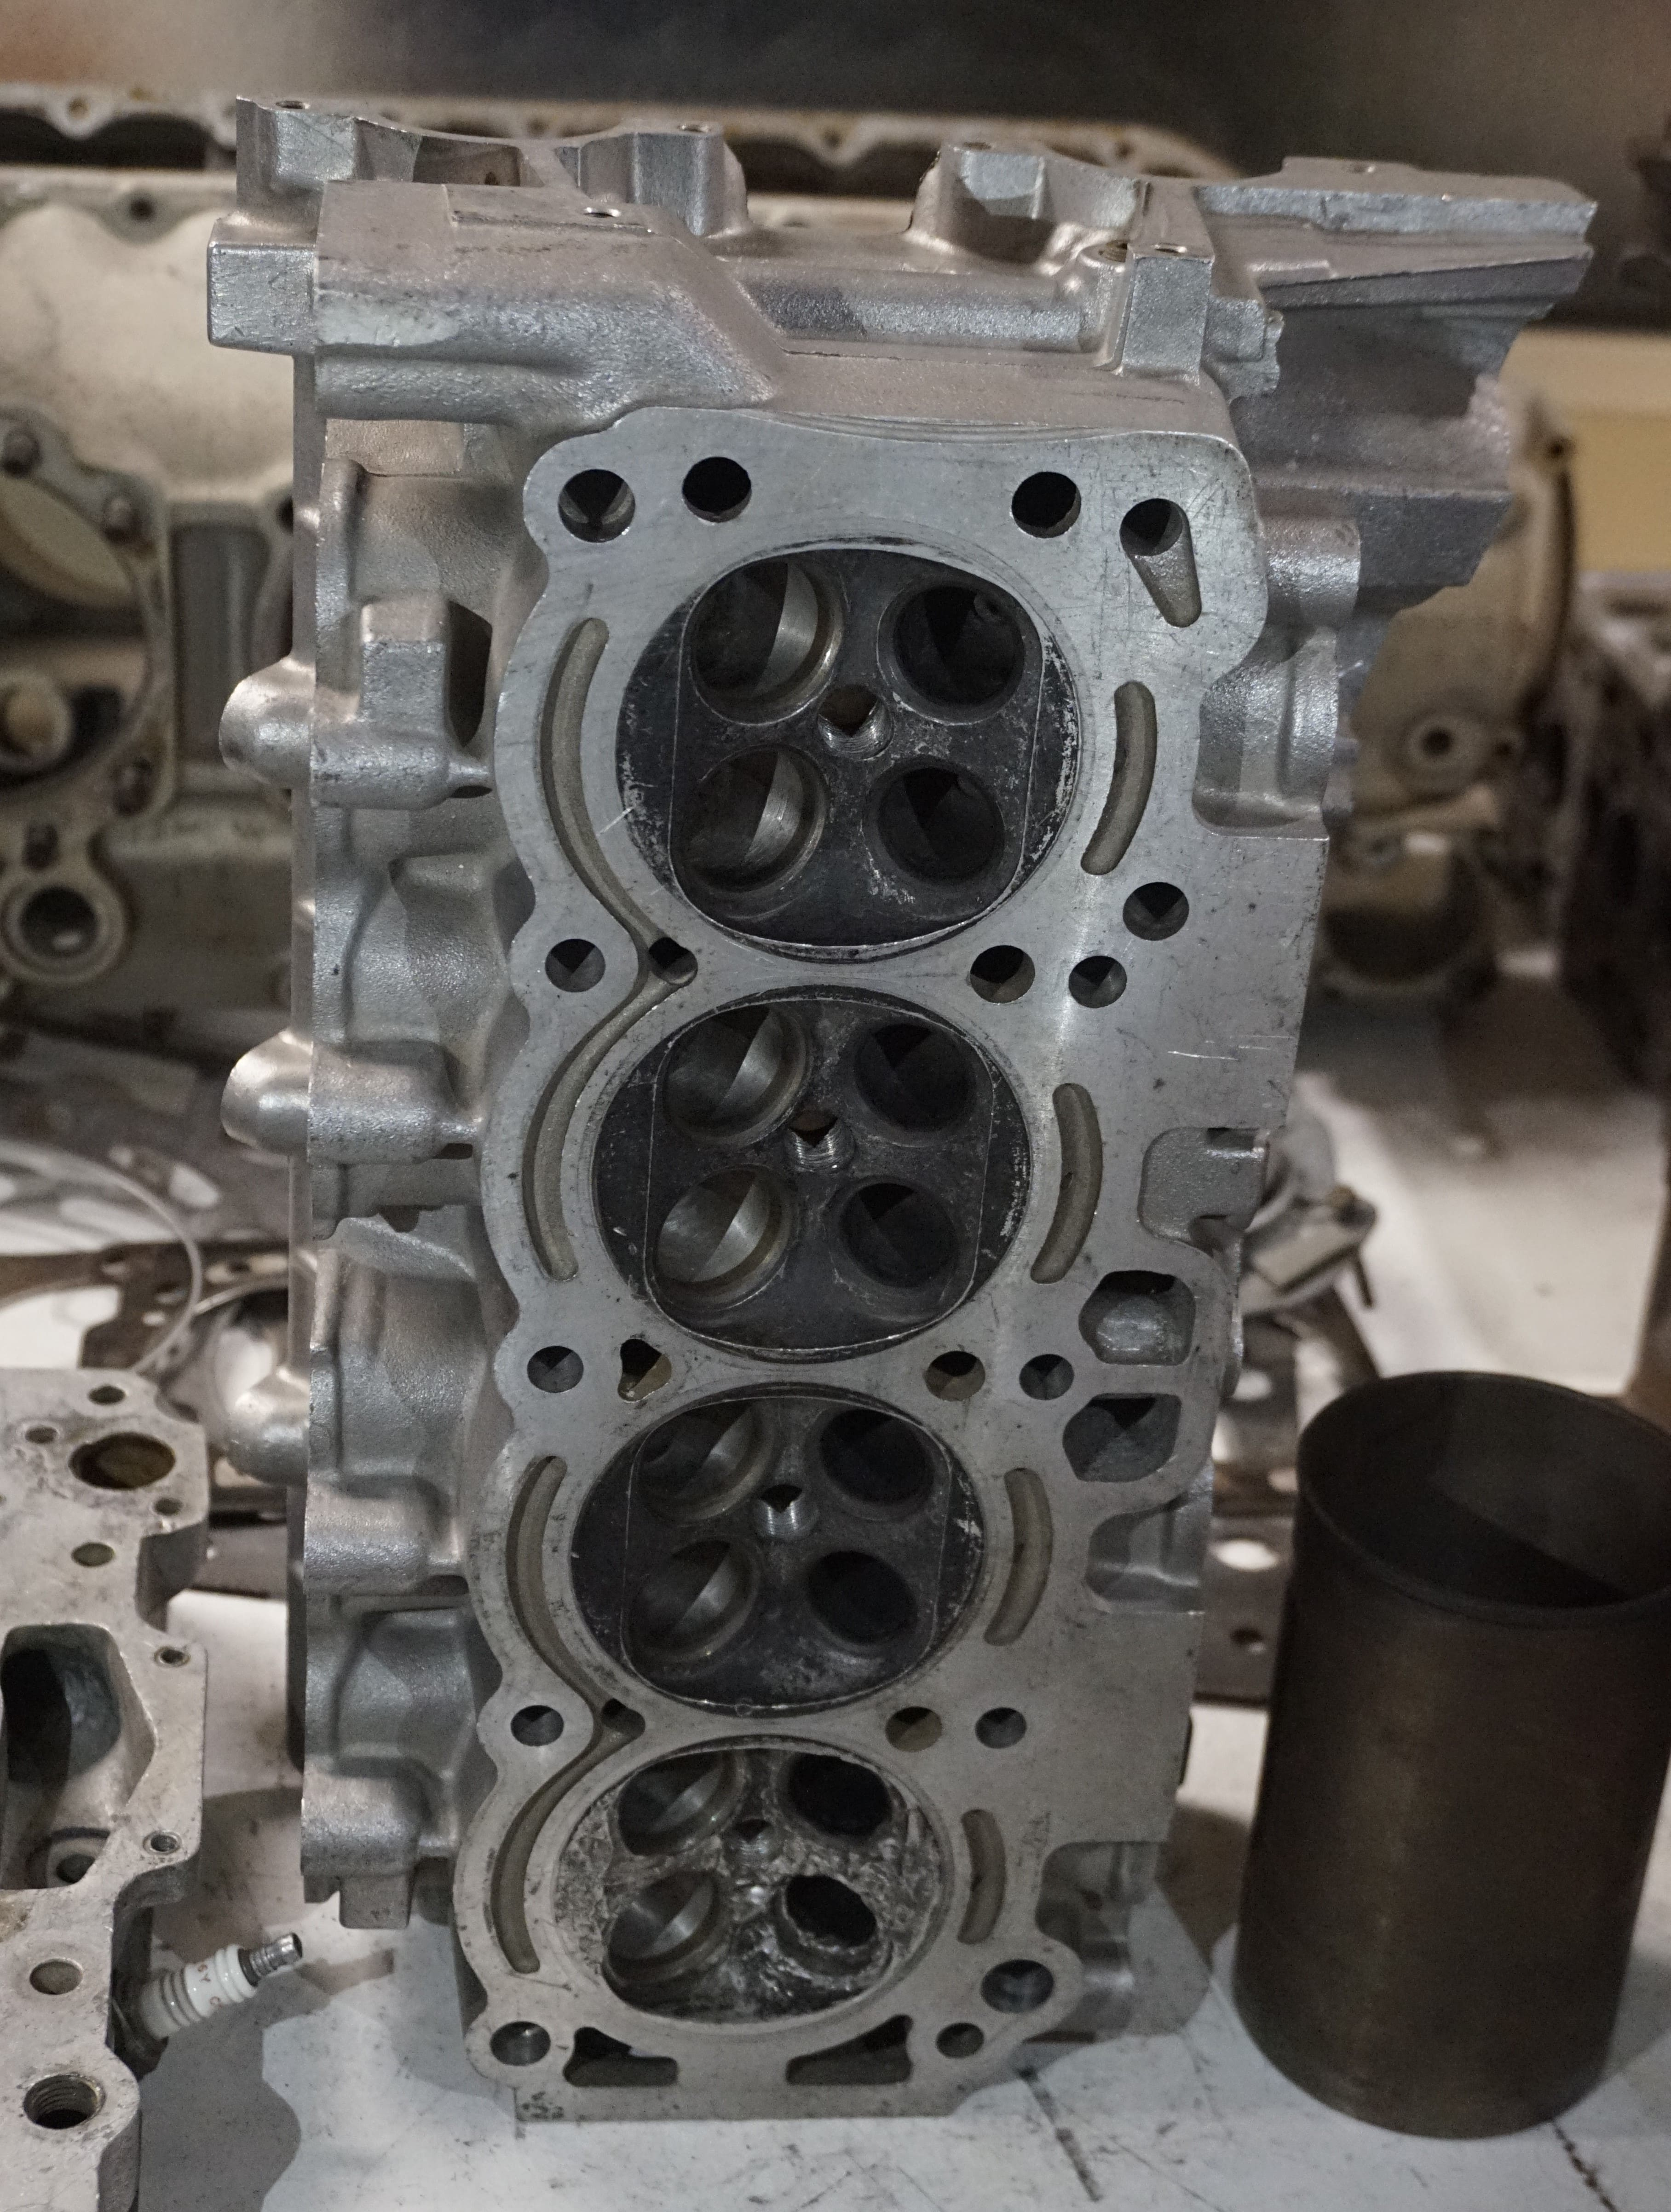
\includegraphics[width=0.65\linewidth]{Figures/02/m3/petrol_head.jpg}
        \caption{Motor Otto.}
        \label{fig:C_gas}
    \end{subfigure}
    \hfill
    \begin{subfigure}[b]{0.45\textwidth}
        \centering
        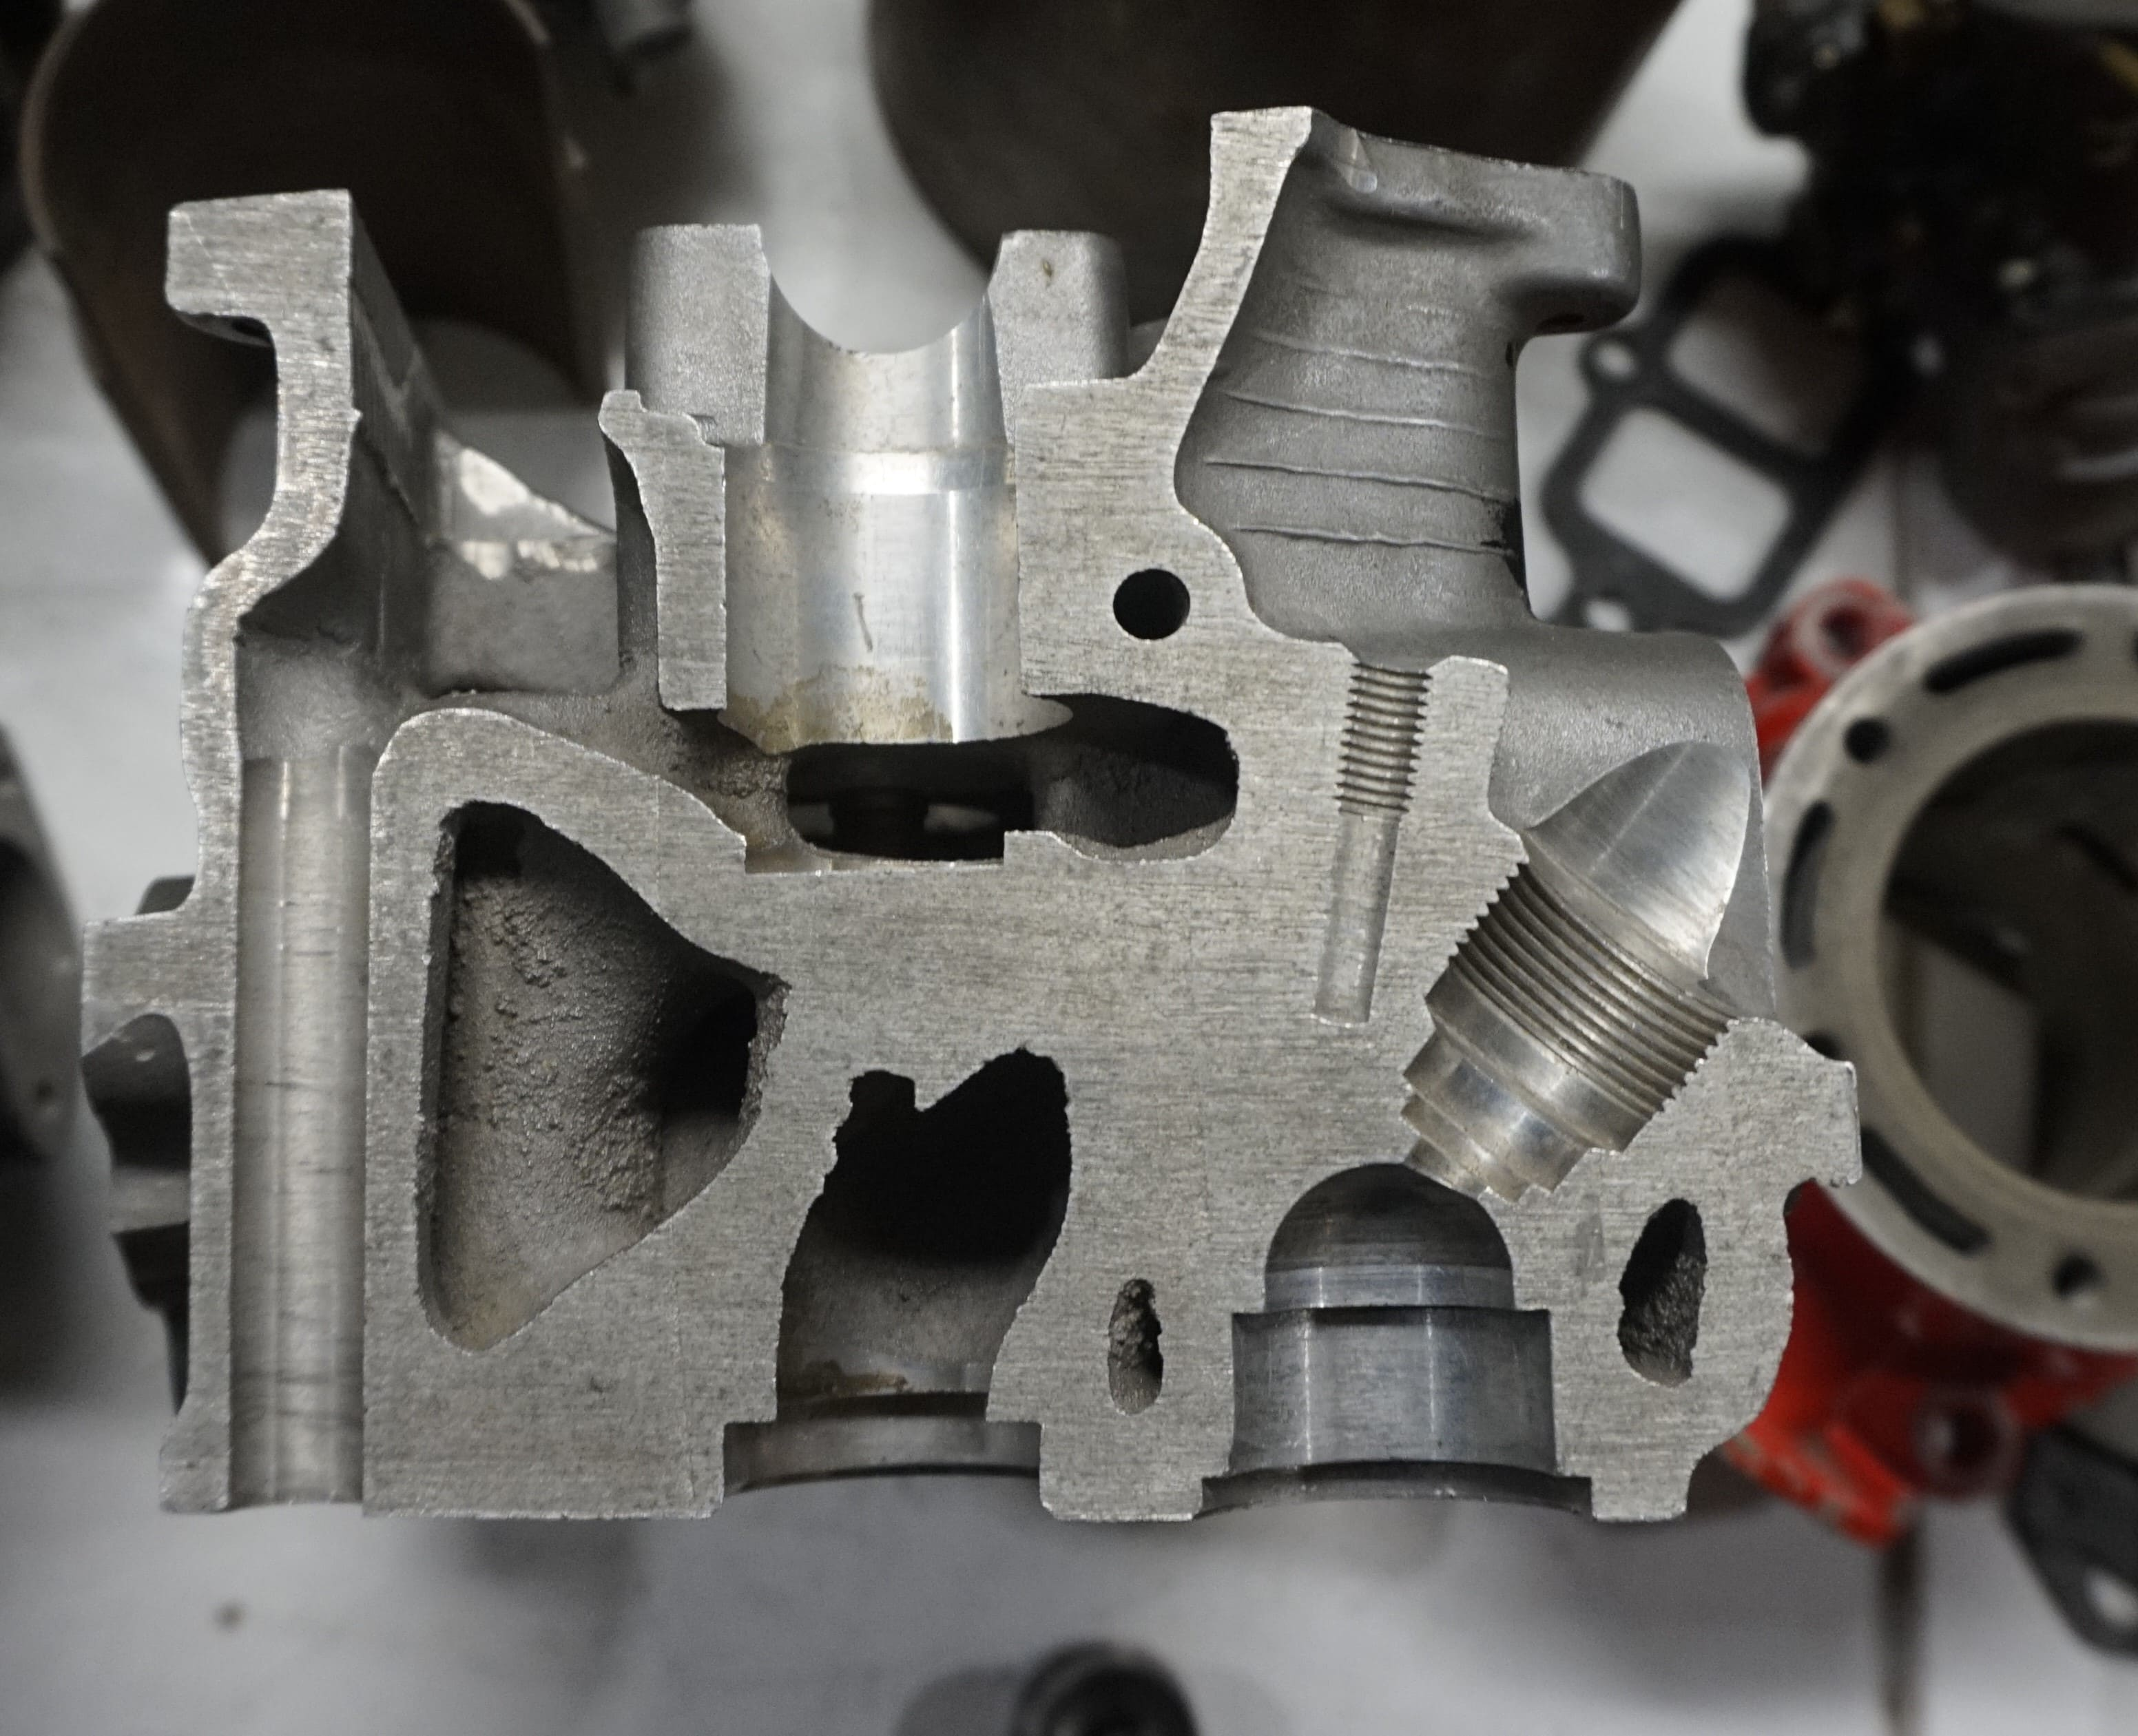
\includegraphics[width=\linewidth]{Figures/02/m3/diesel_head.jpg}
        \caption{Motor Diésel.}
        \label{fig:C_diesel}
    \end{subfigure}    
    \caption{Culatas.}
    \label{fig:C_combined}
\end{figure}

En esta figura \ref{fig:premezcla} en que se observa el inserto que completa la precámara se puede apreciar perfectamente el orificio por el que se llena de aire (y se extrae la mezcla aire-combustible) esta cámara. La geometría de dicho orificio se escoge para dar la cantidad correcta de turbulencia al fluido de manera que se pueda producir correctamente el quemado del diésel en el pistón y, por tanto, se obtenga el correcto funcionamiento del motor.

\begin{figure}[H]
	\centering
	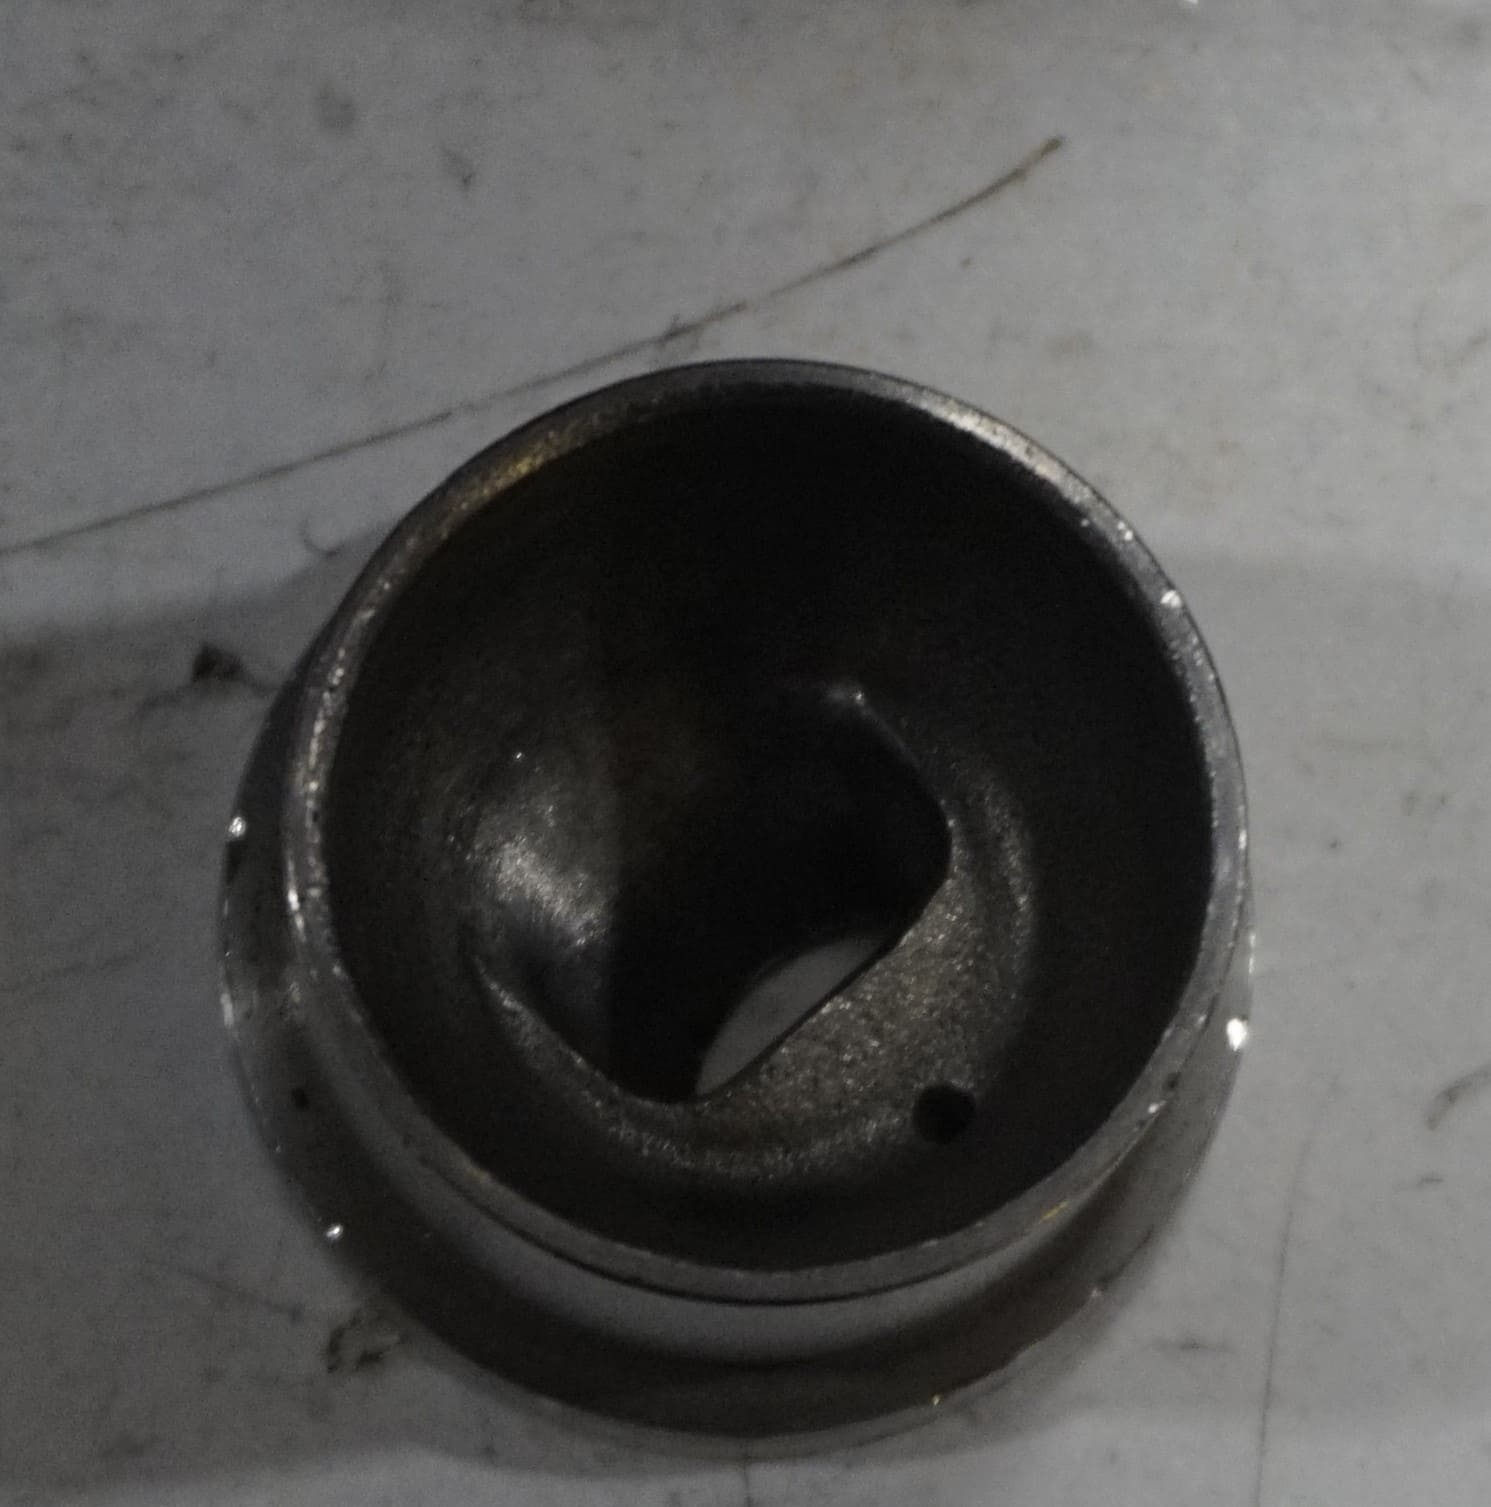
\includegraphics[width=0.6\linewidth]{Figures/02/m3/premix.jpg}
	\caption{Inserto para completar la precámara.}
	\label{fig:premezcla}
\end{figure}

En cuanto al resto de accesorios alojados en la culata, en las imágenes \ref{fig:head_val} y \ref{fig:head_spark} se puede ver la instalación en la culata respectivamente de las válvulas de admisión y escape (con sus mecanismos de retención y de retorno al cierre mediante muelles) y la bujía (en una culata de un motor gasolina).

\begin{figure}[H]
	\centering
	\begin{subfigure}[b]{0.45\textwidth}
		\centering
		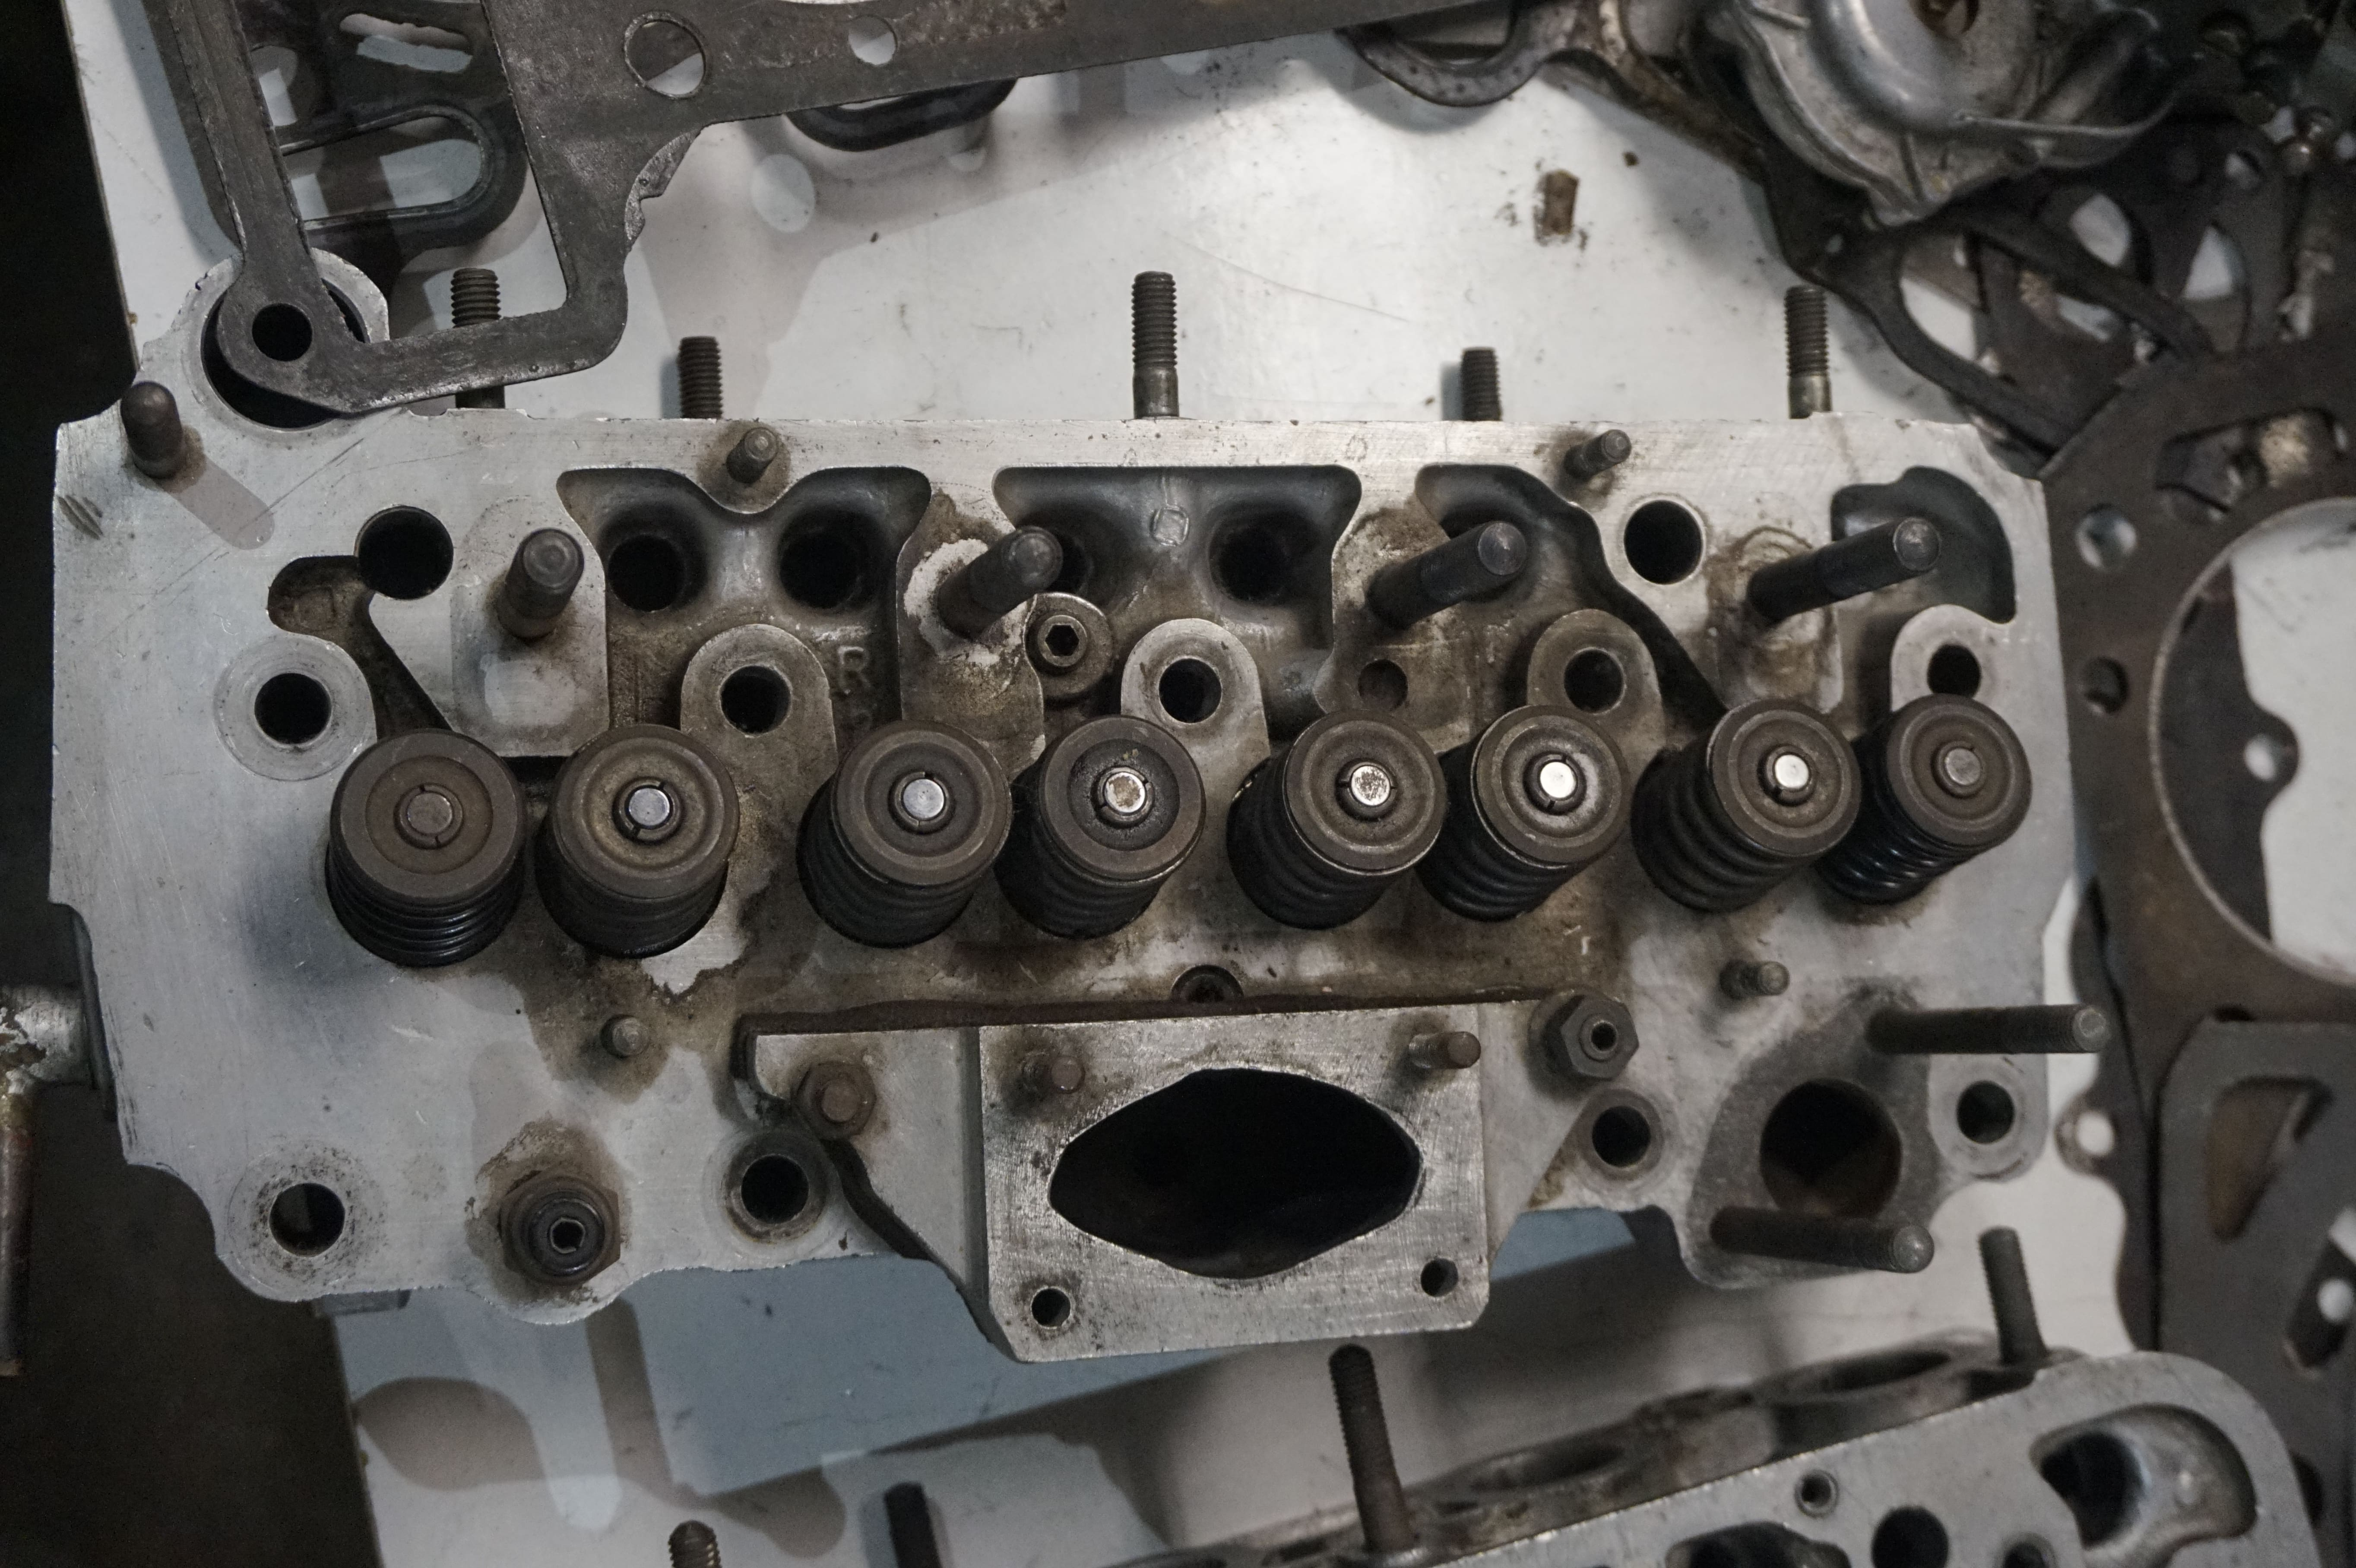
\includegraphics[width=\linewidth]{Figures/02/m3/head_top_val.jpg}
		\caption{Válvulas instaladas en la culata.}
		\label{fig:C_gas}
	\end{subfigure}
	\hfill
	\begin{subfigure}[b]{0.45\textwidth}
 		\centering
 		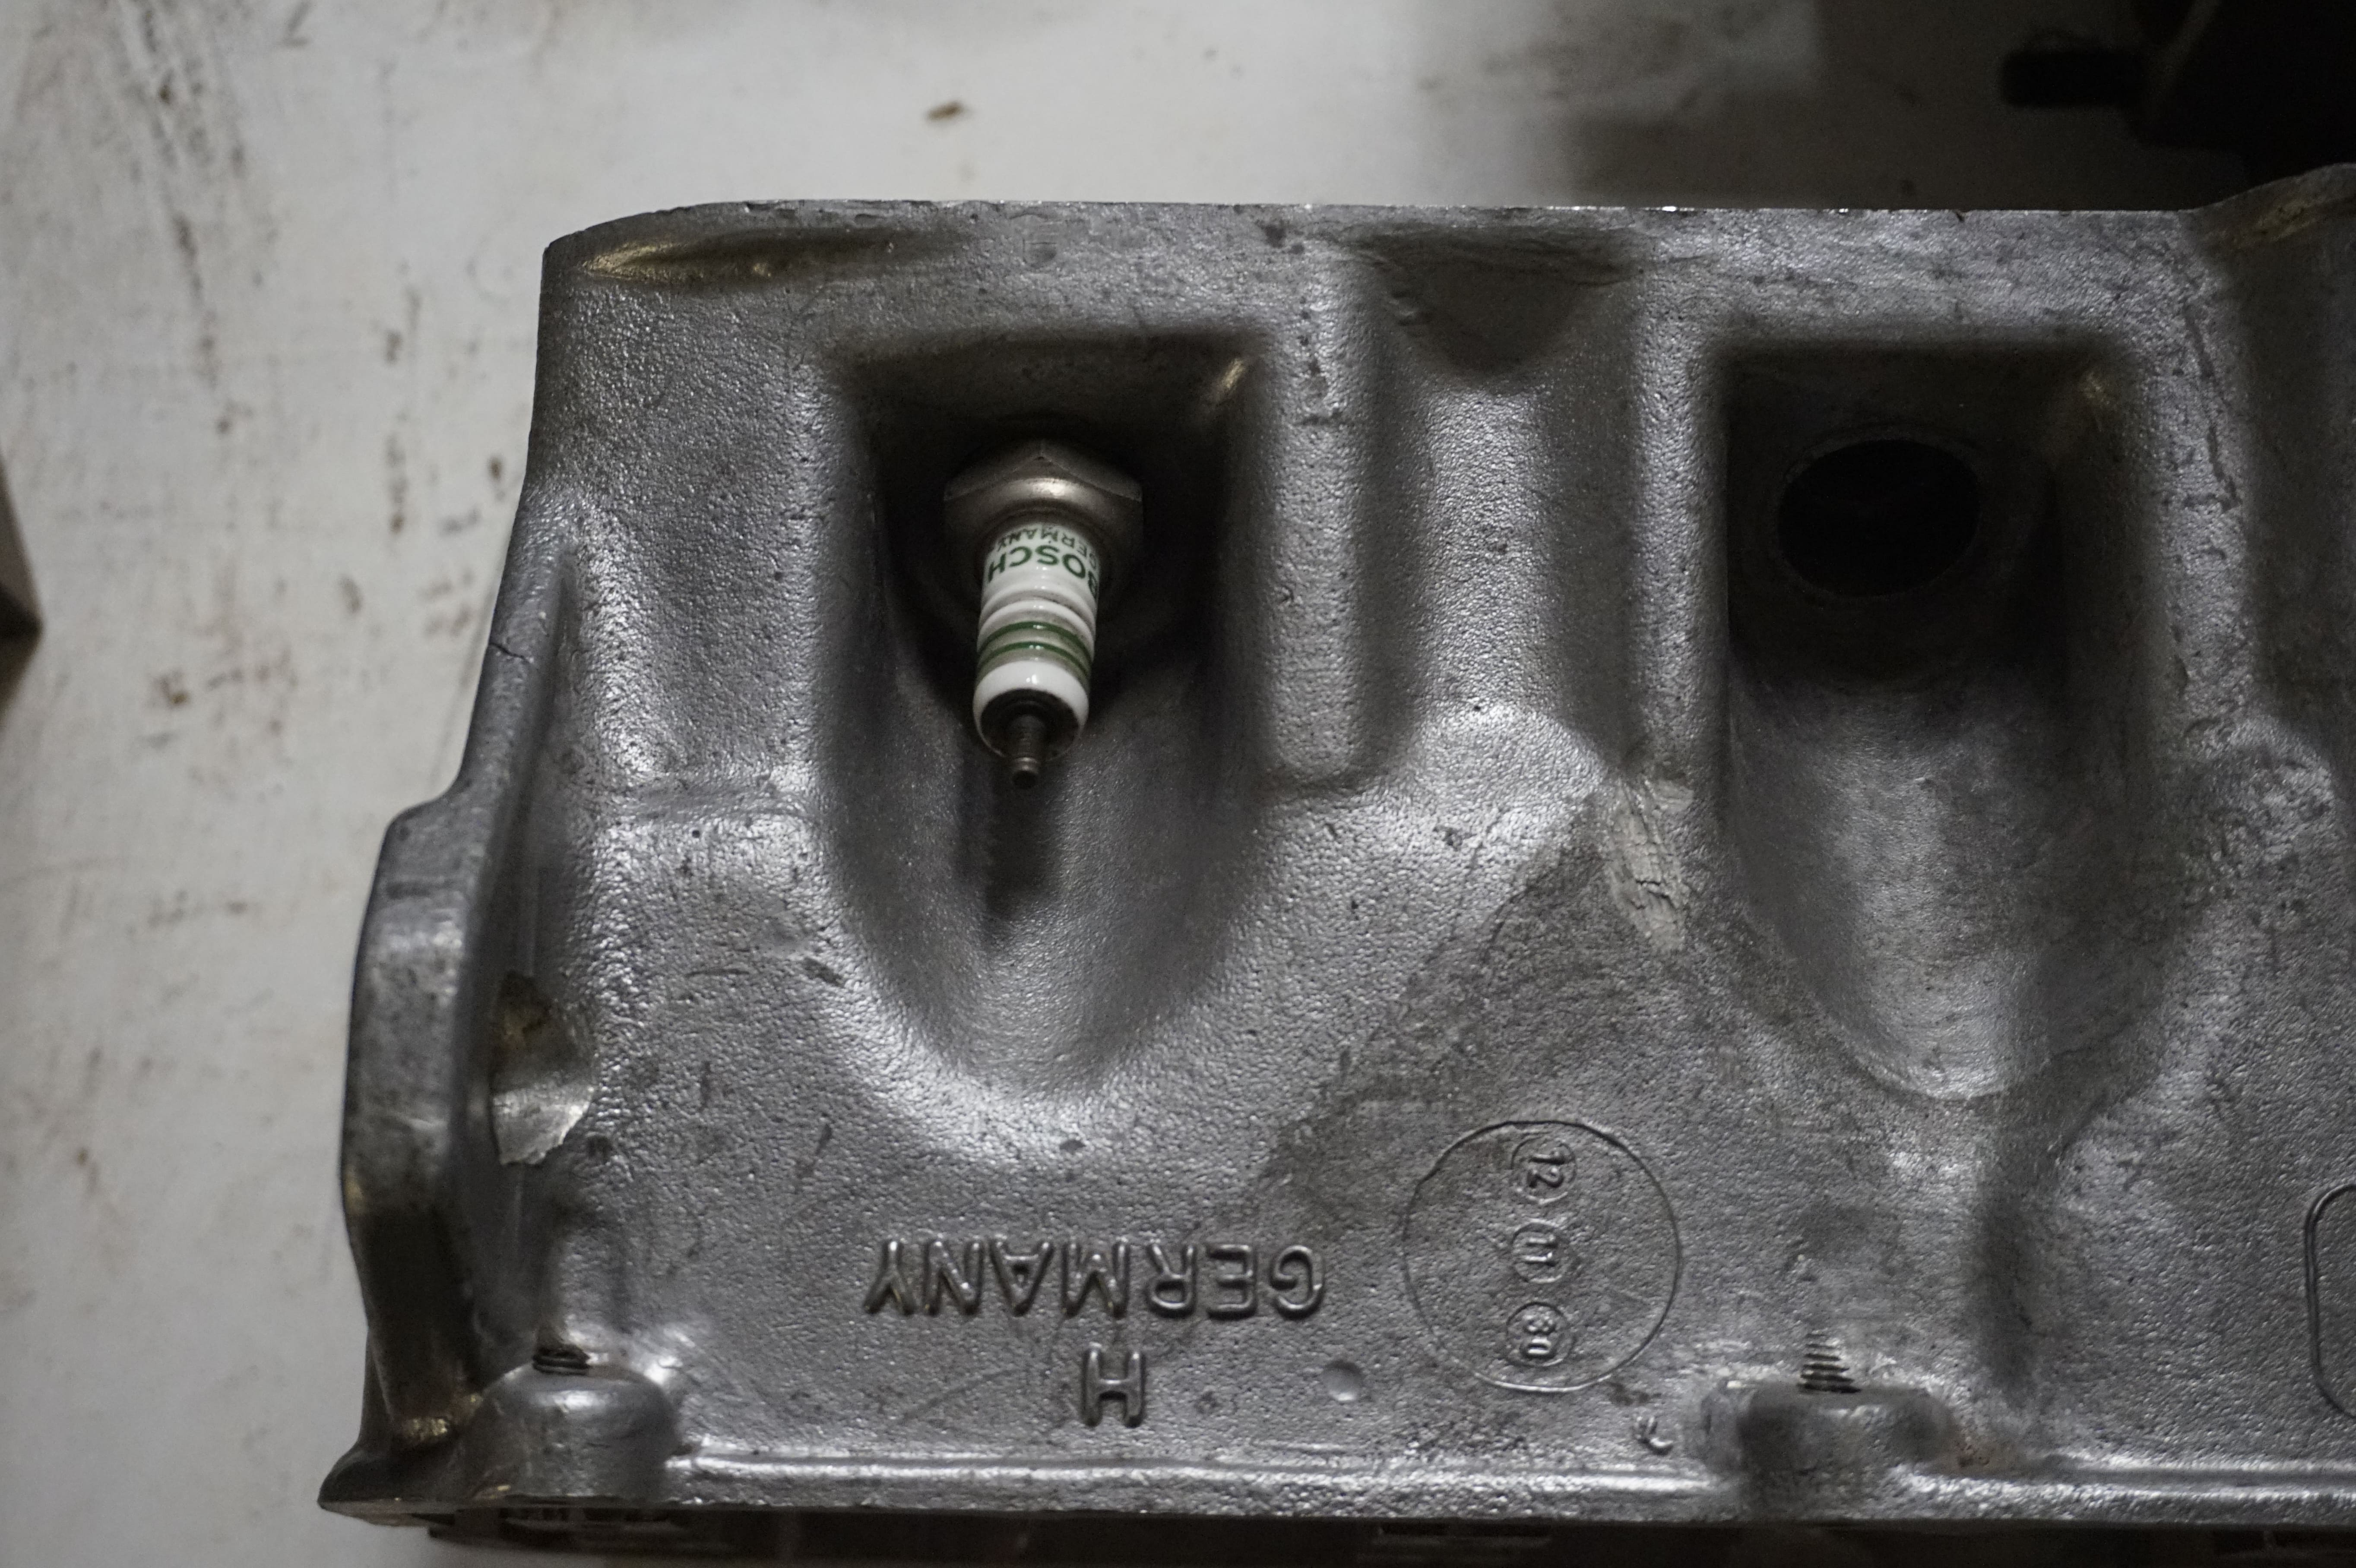
\includegraphics[width=\linewidth]{Figures/02/m3/head_sparkplug.jpg}
 		\caption{Bujía instalada en su alojamiento.}
		\label{fig:C_diesel}
	\end{subfigure}    
	\caption{Accesorios en la culata.}
	\label{fig:C_accesory}
\end{figure}

\subsection{Bloque motor} \label{ss:bloque}

En el siguiente grupo de imágenes se observan dos bloques motor, en el caso de la figura \ref{fig:bloq_bmw} se aprecia la segunda bancada (cilindros 6 a 10) del bloque de un motor BMW S85 (normalmente instalado en los BMW M5 E60), fabricado en aluminio. Dado que el aluminio es un material relativamente \textit{blando}, las superficies laterales de los cilindros han debido de sufrir algún tratamiento superficial que las endurezca, pues en el caso contrario, los segmentos y los propios pistones generarían un desgaste excesivo en el bloque. Además, en esta imagen también se pueden apreciar los canales por los que fluye el refrigerante a través del bloque (aquellos con forma de sector circular y parte de los que tienen sección circular). Estos canales se corresponderán con otros con una configuración idéntica en las juntas de culata y culatas de forma que, junto con el radiador y la bomba de agua, se termina de cerrar el circuito de refrigeración.\\

En la figura \ref{fig:bloq_cig} se observa la parte inferior de un bloque motor de cuatro cilindros en línea, especialmente los alojamientos de los cojinetes de apoyo del cigüeñal, con un canal mecanizado en el centro de todos ellos para suministrar el aceite lubricante necesario para el correcto funcionamiento del motor y asegurar la durabilidad del mismo.\\

\begin{figure}[H]
	\centering
	\begin{subfigure}[b]{0.45\textwidth}
		\centering
		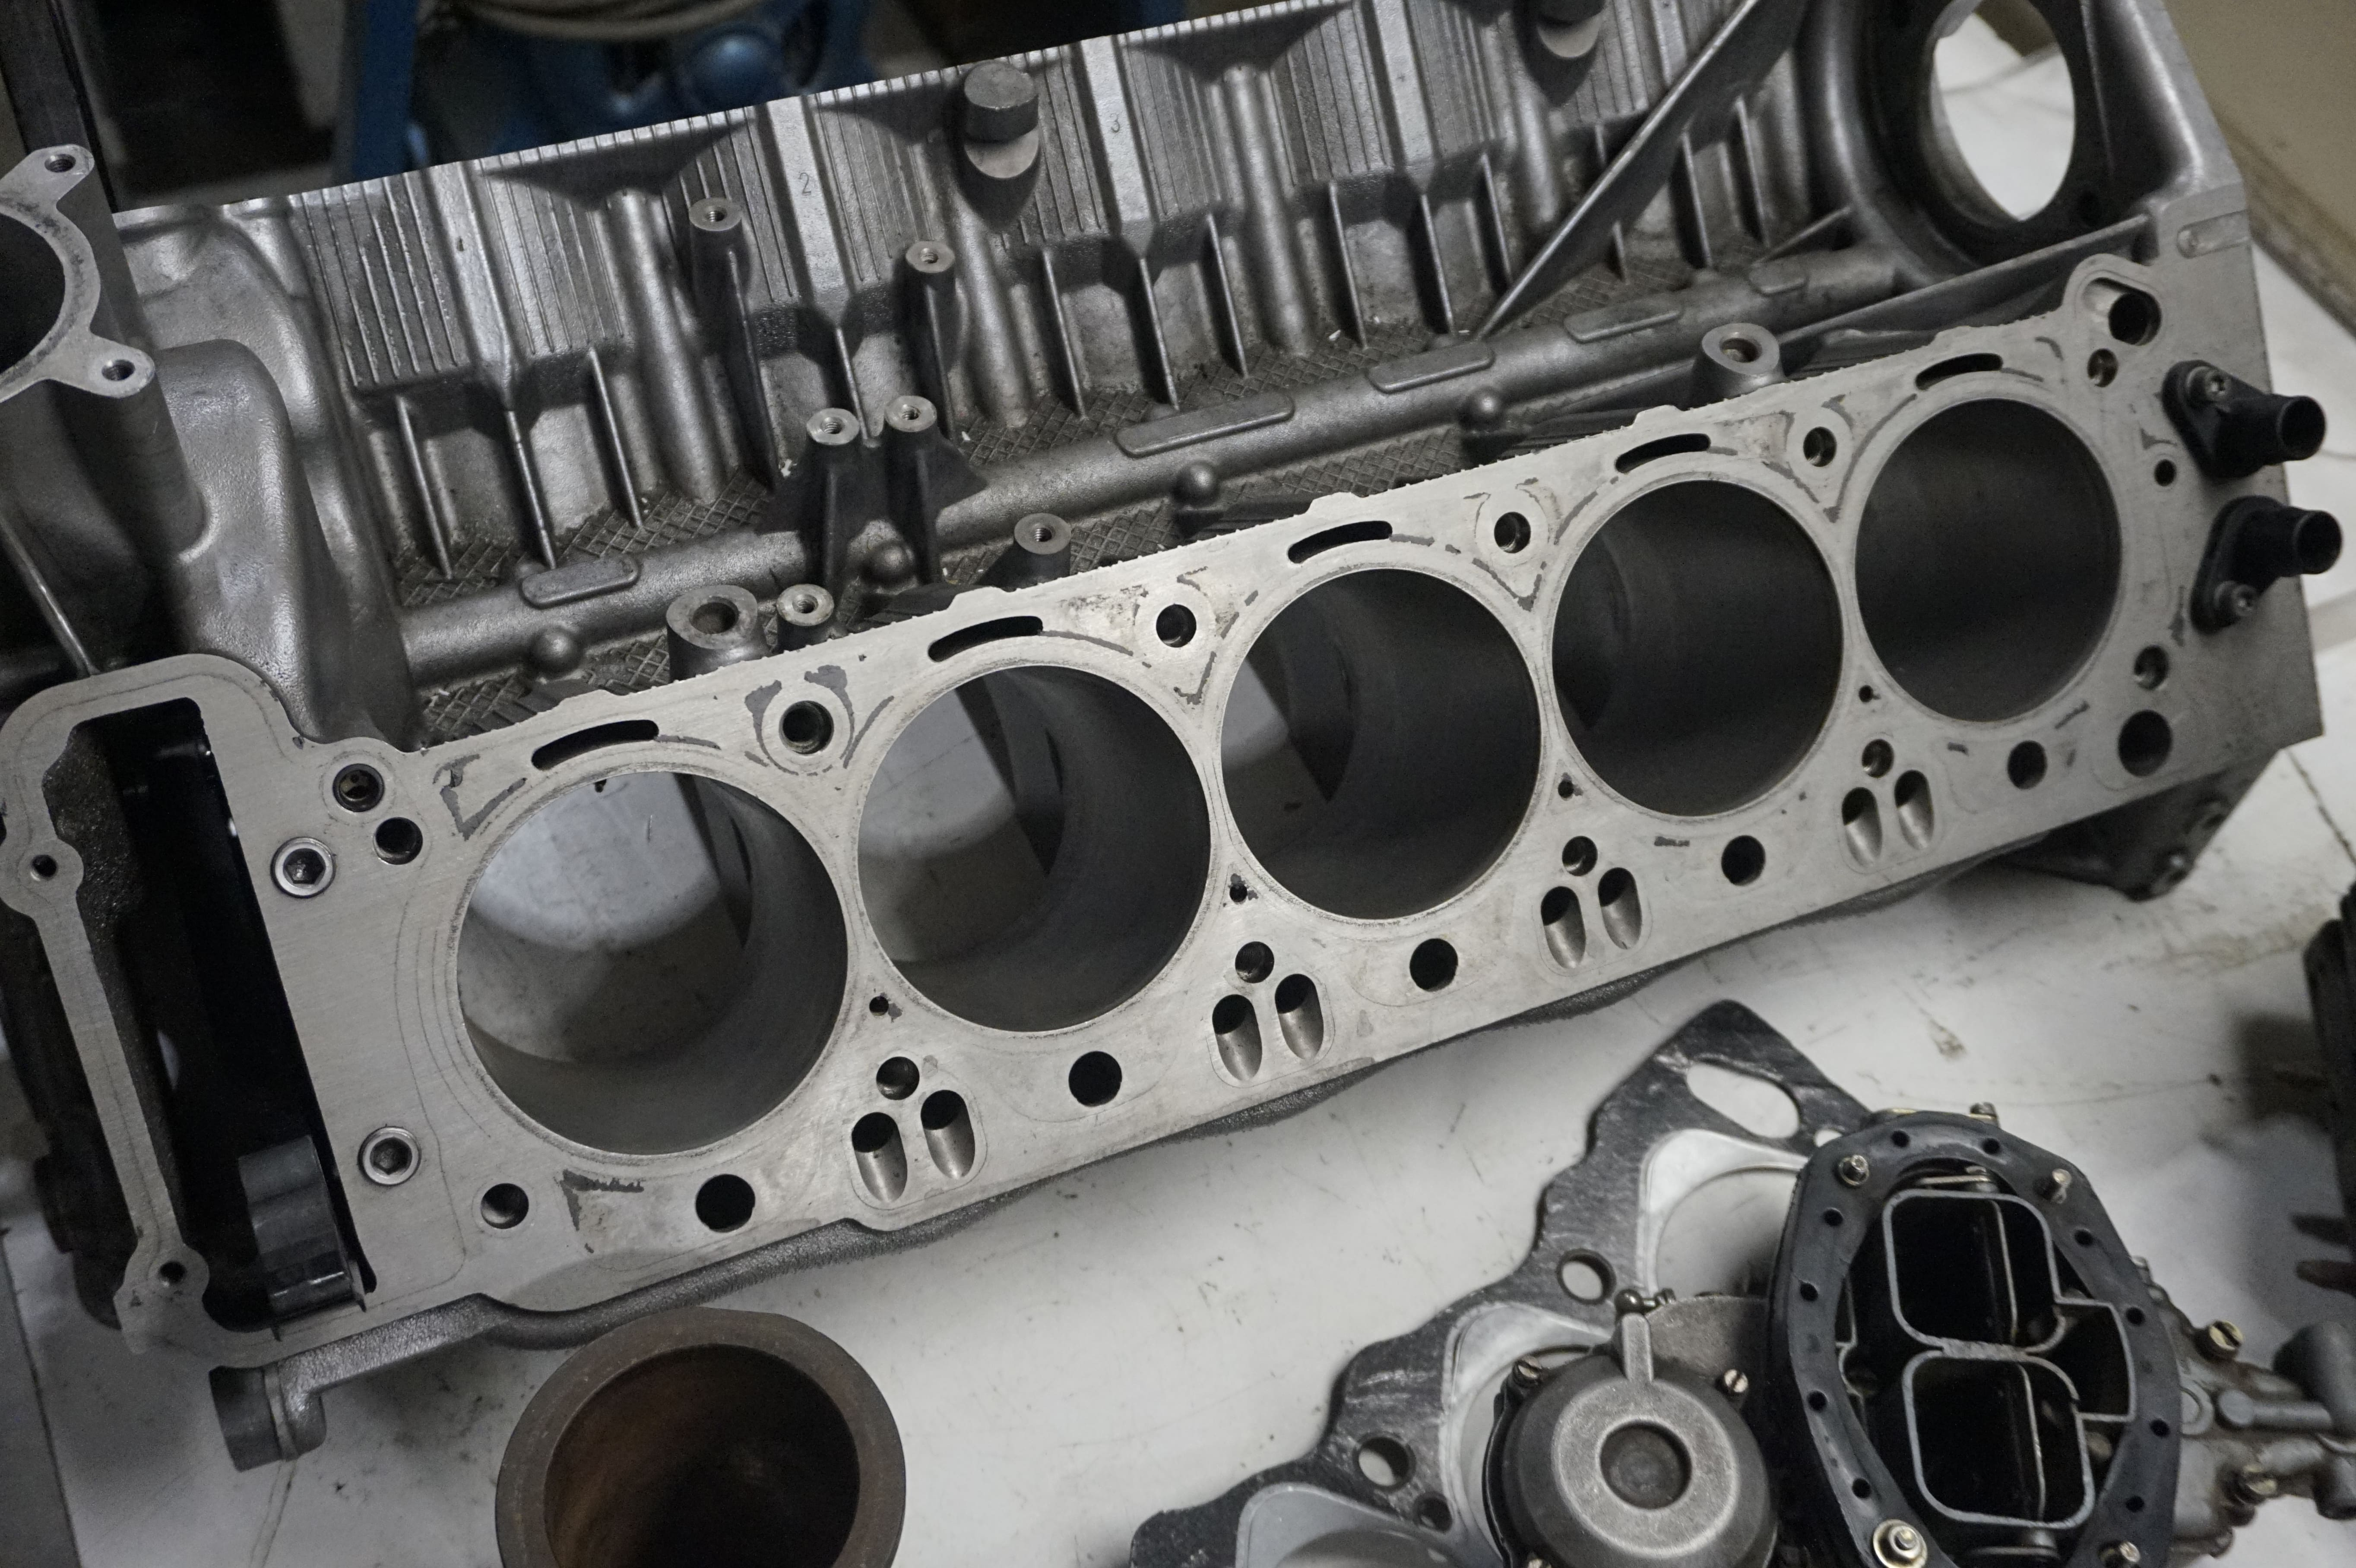
\includegraphics[width=\linewidth]{Figures/02/m3/bloq_bmw_2.jpg}
		\caption{Bloque BMW S85.}
		\label{fig:bloq_bmw}
	\end{subfigure}
	\hfill
	\begin{subfigure}[b]{0.45\textwidth}
 		\centering
 		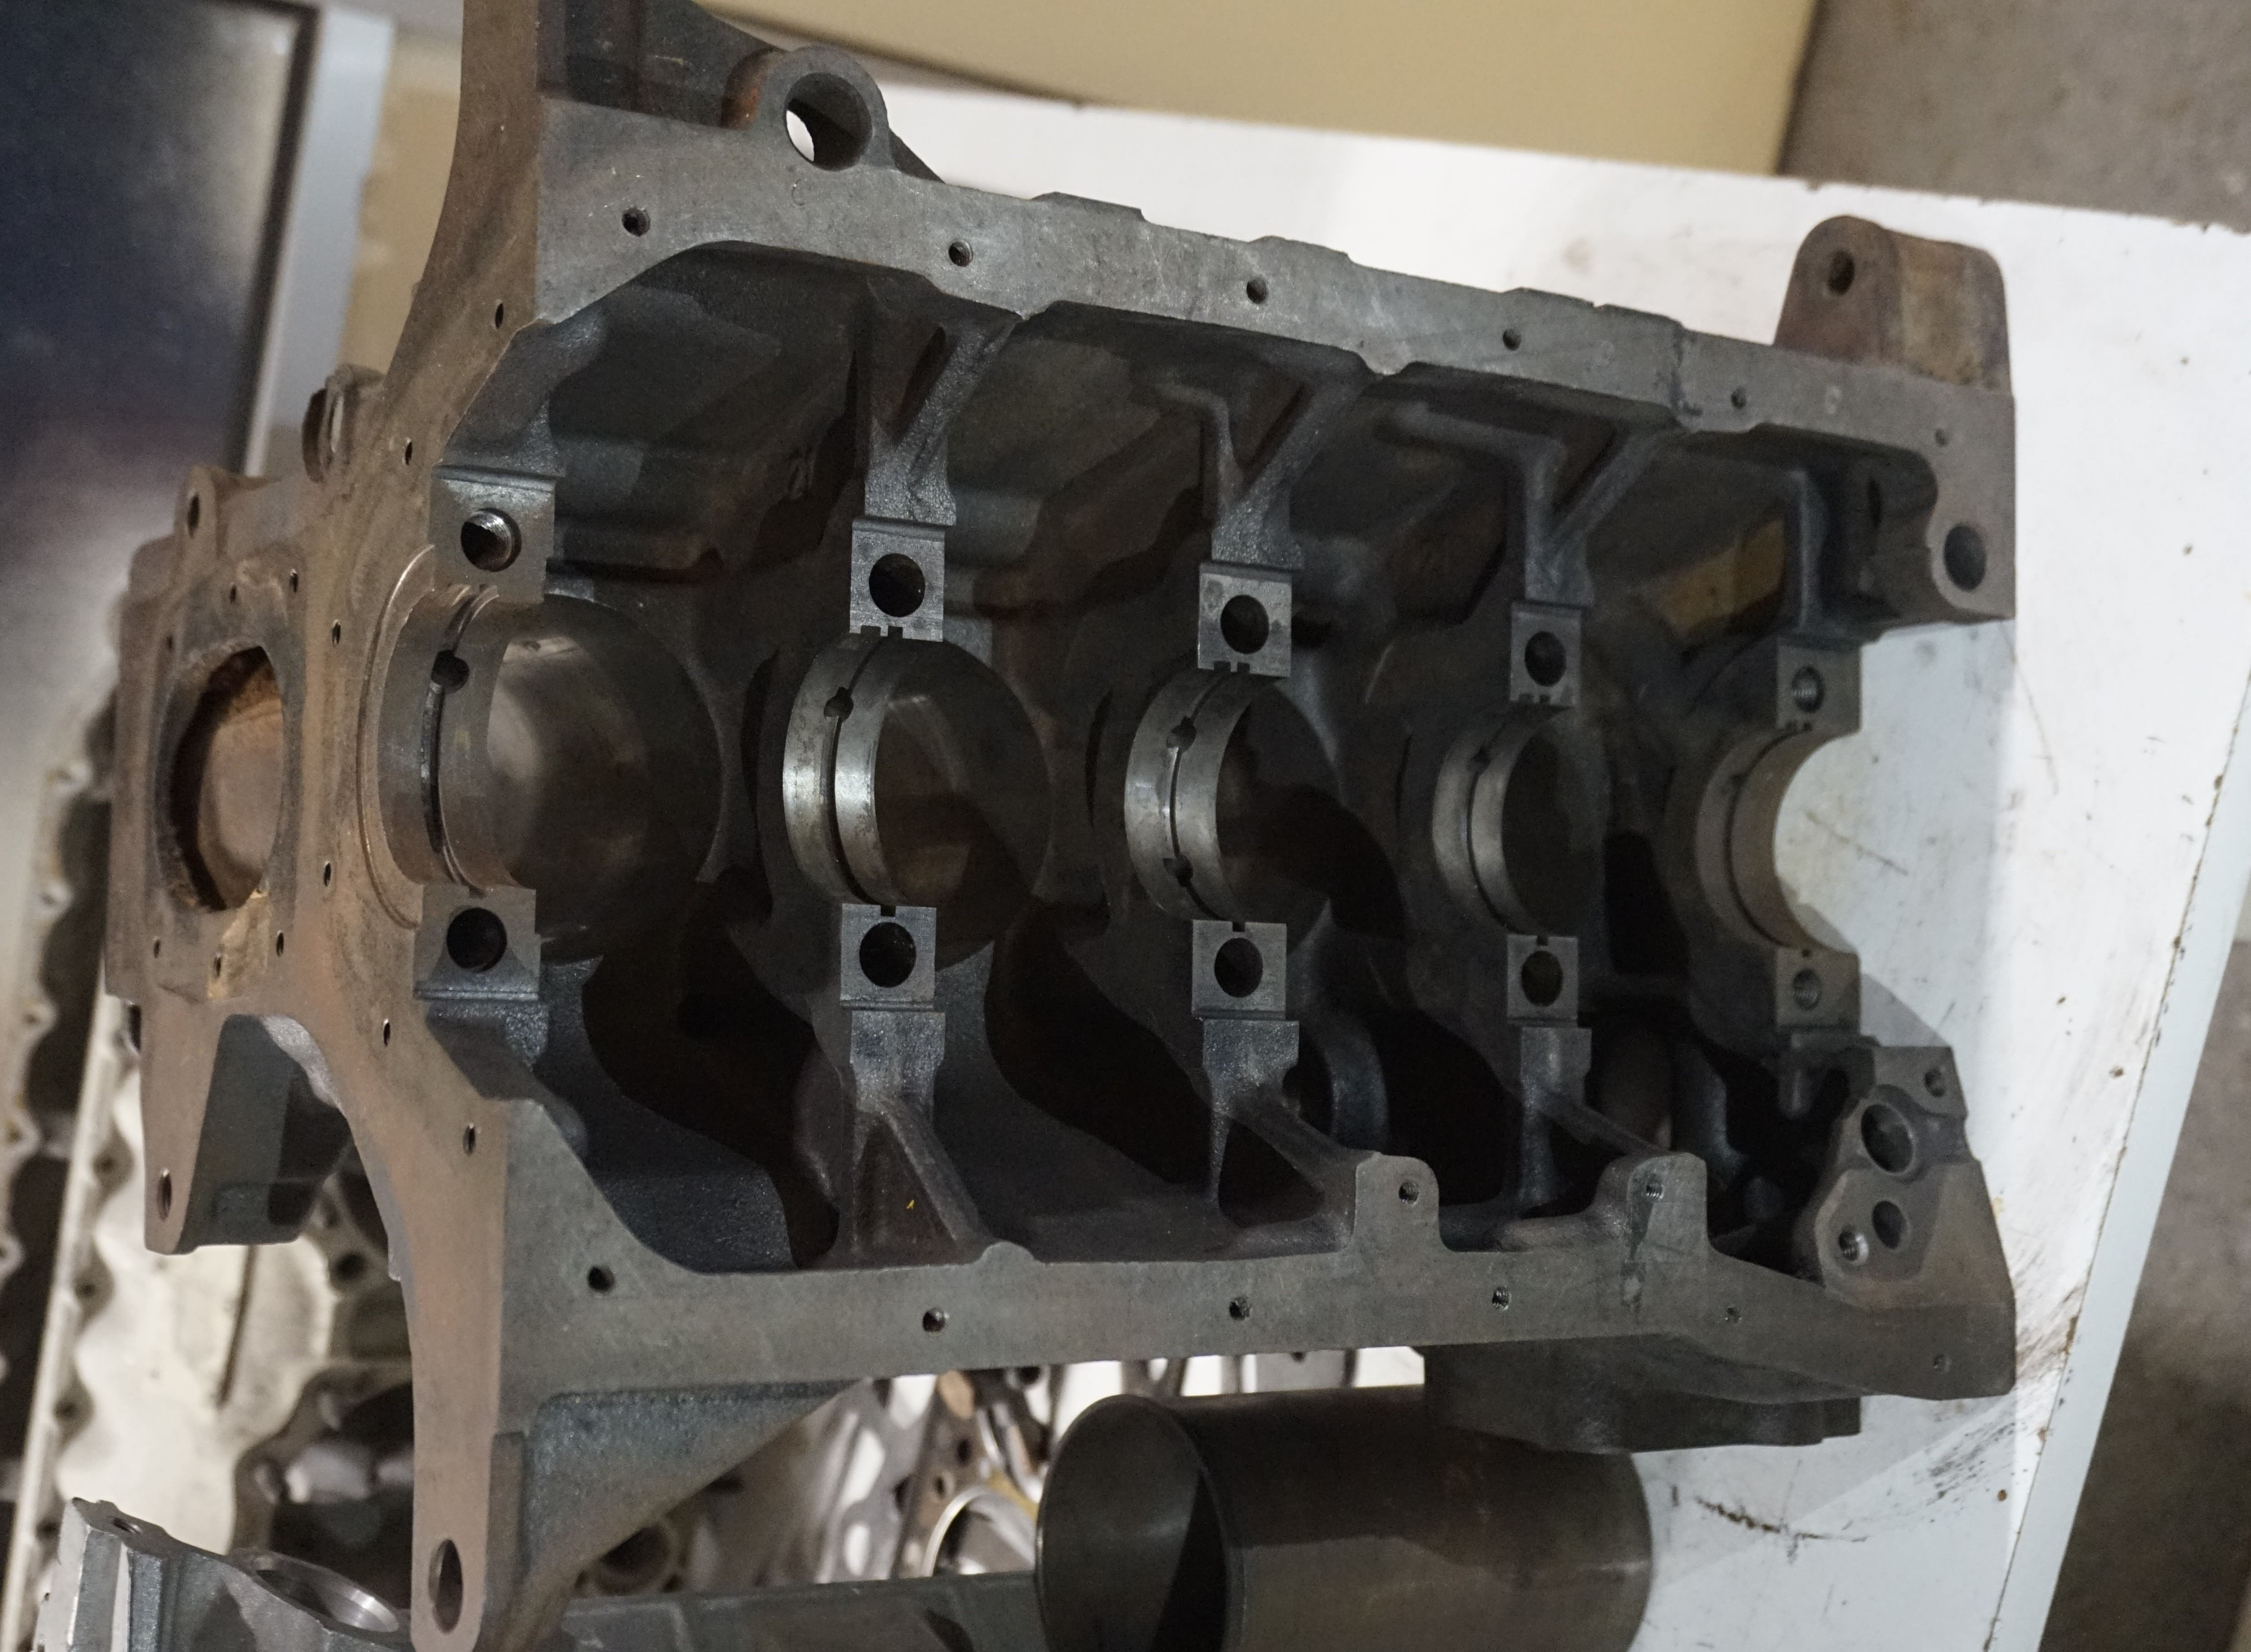
\includegraphics[width=\linewidth]{Figures/02/m3/bloq_cig.jpg}
 		\caption{Apoyos del cigüeñal.}
		\label{fig:bloq_cig}
	\end{subfigure}    
	\caption{Accesorios en la culata.}
	\label{fig:auto_block}
\end{figure}

Más allá de estos motores de uso automovilístico, es interesante observar en la imagen \ref{fig:crankcase} el cárter central al que se anclan los cilindros en un motor bóxer (de cilindros opuestos) de 6 cilindros. Se observa que se encuentra dividido a la mitad, ya que se han de instalar piezas a ambos lados del cigüeñal. Además, al tratarse de piezas de un motor aeronáutico, es interesante observar que la cantidad de material utilizado, respecto a los motores vistos anteriormente es menor, con el objetivo de mejorar la compacidad de la planta de potencia.

\begin{figure}[H]
	\centering
	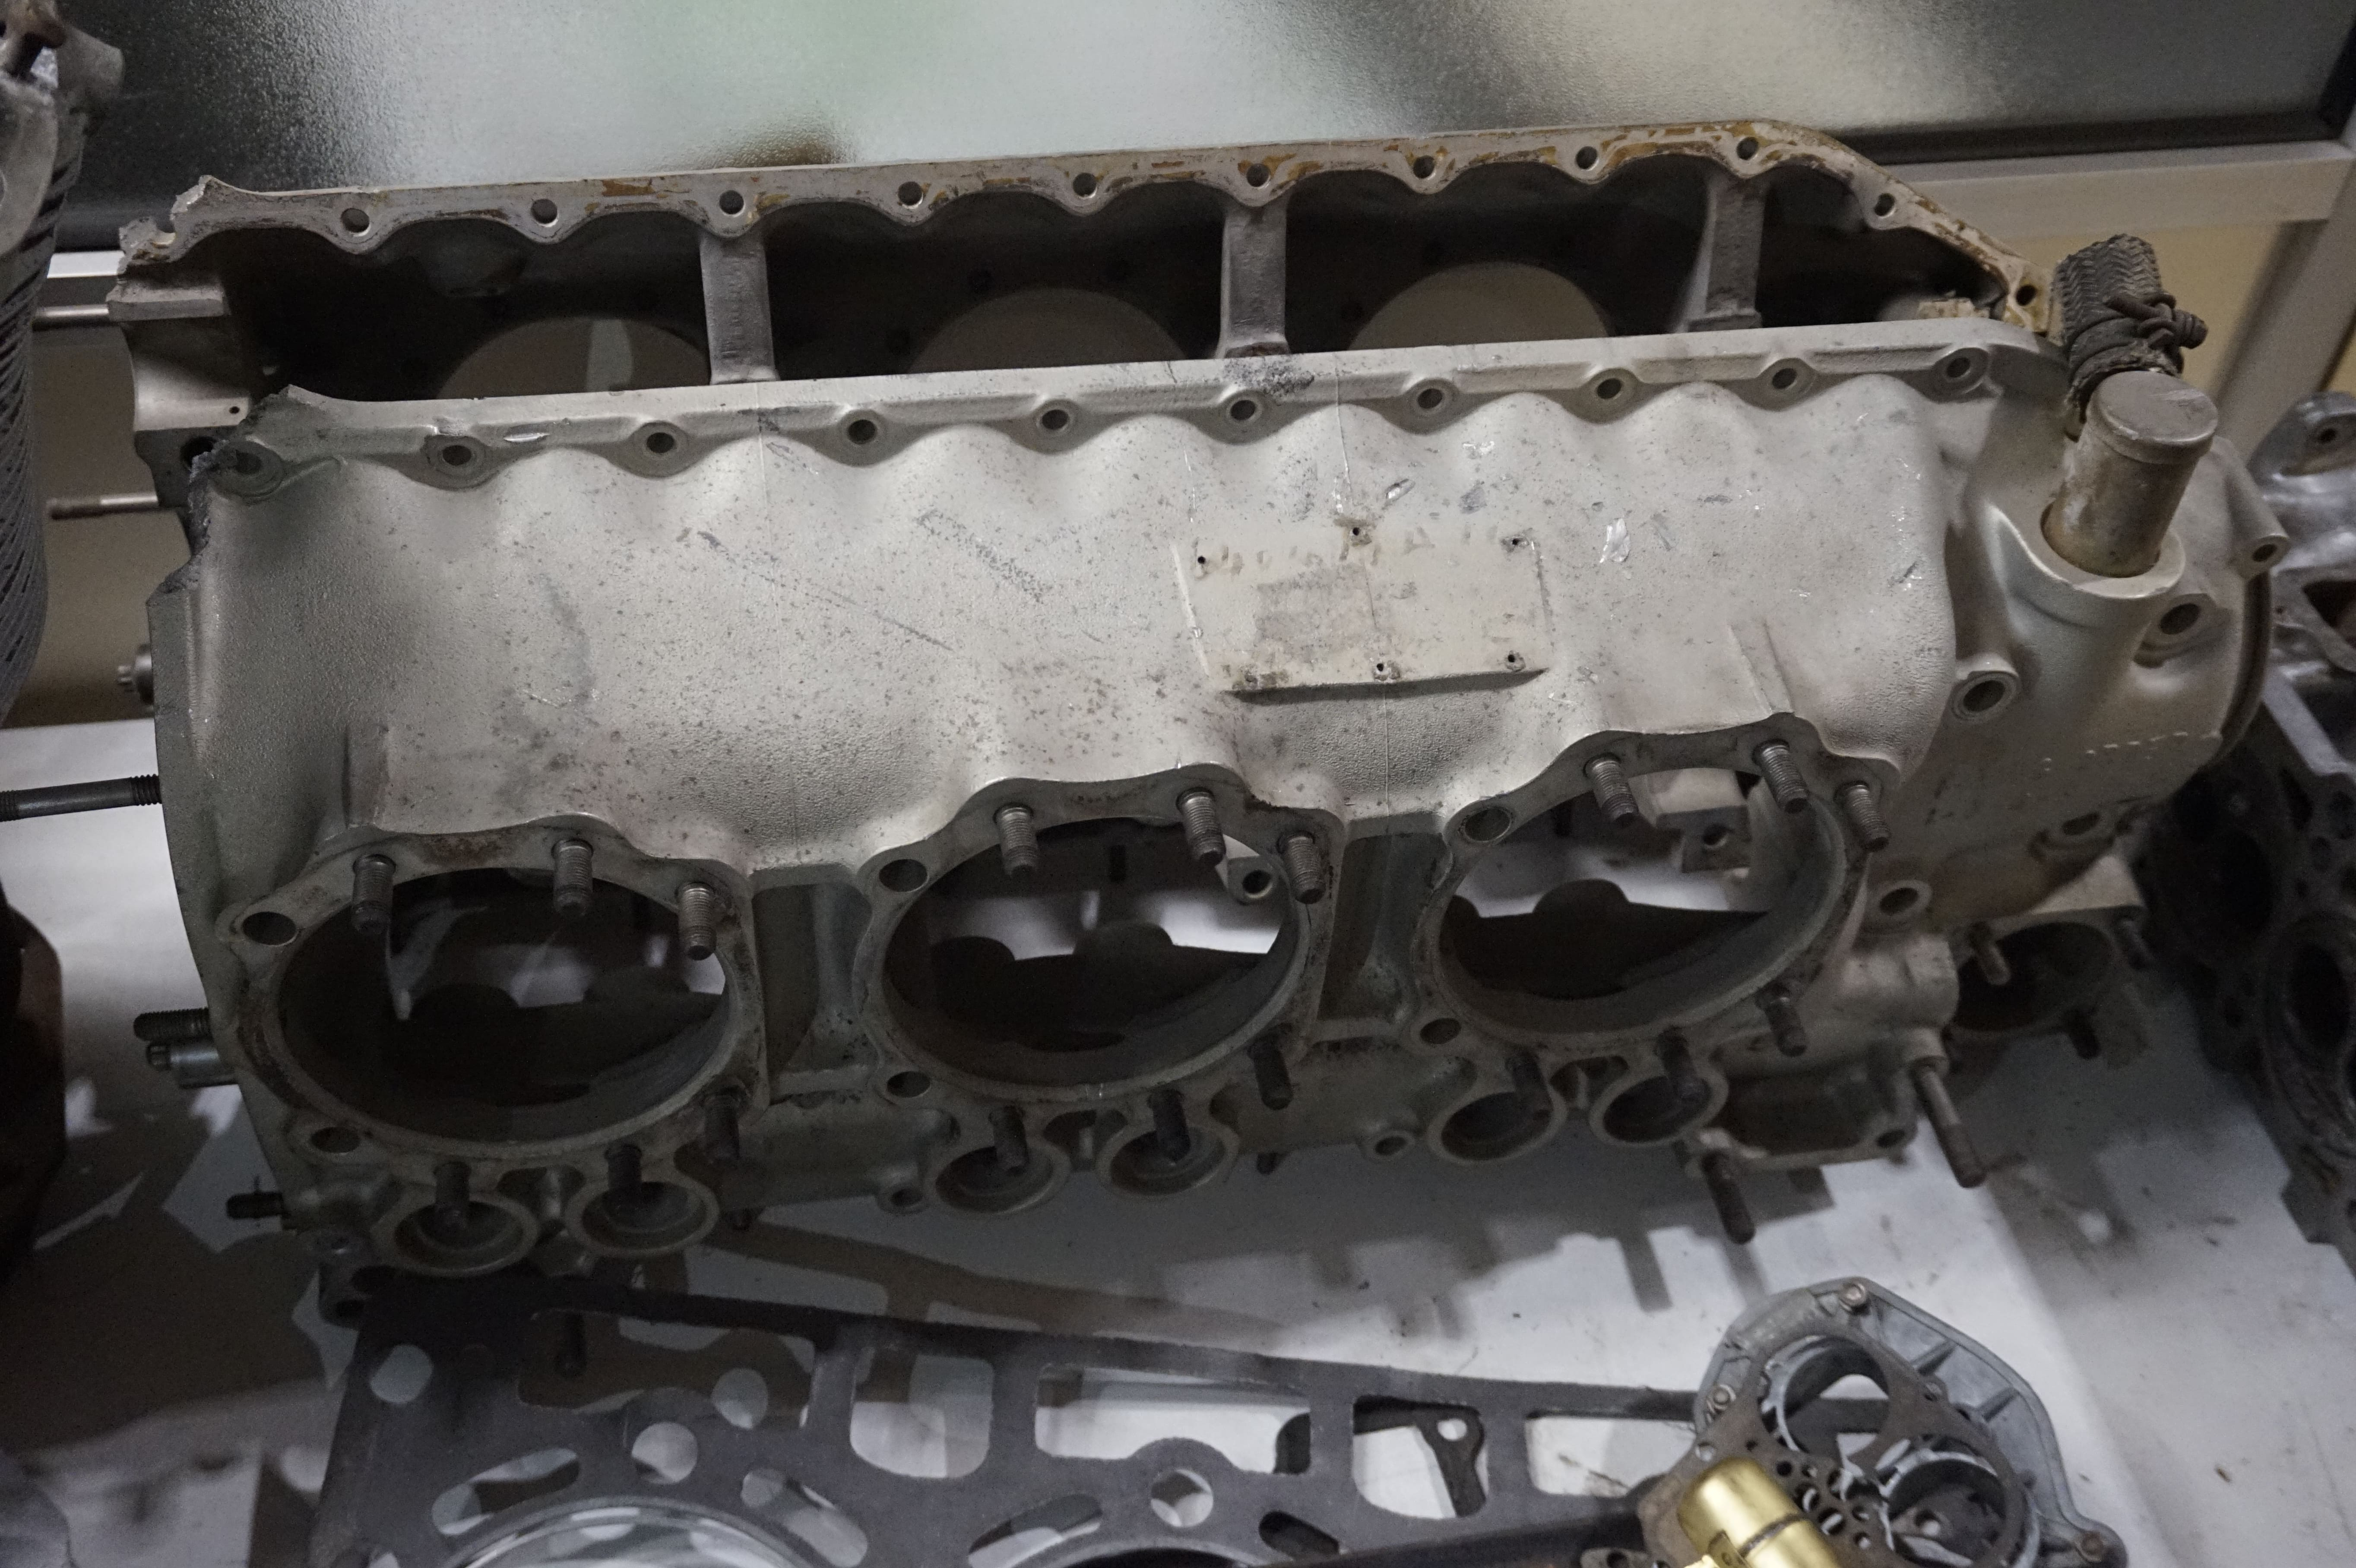
\includegraphics[width=0.6\linewidth]{Figures/02/m3/bloq_boxer.jpg}
	\caption{Cárter de motor aeronáutico}
	\label{fig:crankcase}
\end{figure}

\subsection{Camisas} \label{ss:jacket}

En el caso de que los cilindros estén provistos de camisas, estas pueden ser secas o húmedas. Las camisas secas no se encuentran en contacto con el líquido refrigerante, por lo que un fallo de la camisa (grieta o similar) no llevará a una fuga de refrigerante hacia el cilindro con la gran cantidad de problemas que ello conllevaría. Sin embargo, estas camisas secas tienen un comportamiento algo inferior en lo que a la refrigeración del pistón se refiere (se ha de conducir el calor a través de la camisa, luego al bloque, y de ahí al refrigerante).\\

En cuanto a las camisas húmedas, la refrigeración es algo mejor, pues la camisa está directamente en contacto con el refrigerante (lo cuál es cierto que puede llevar a el deterioro de la misma por motivos de corrosión en algunos casos).

\subsection{Motor radial} \label{ss:cil_rad}

Los motores radiales fueron utilizados en grandes cantidades a lo largo de la Segunda Guerra Mundial, gracias a la posibilidad que ofrecían de situar un mayor número de cilindros con longitudes de los motores más reducidas. Otro beneficio que presentan es que es más sencillo refrigerarlos por aire, y es por eso que en el cilindro que se observa en la figura \ref{fig:cil_rad} se aprecia una gran cantidad de aletas cuyo cometido es aumentar la superficie expuesta a la corriente de aire para favorecer dicha refrigeración. Además, al tratarse de motores con válvulas accionadas por varillas, es necesario invertir el movimiento de la varilla para poder abrir la válvula, por lo que se hace necesario alojar (en la posición fotografiada en la figura \ref{fig:bal_rad}) un balancín que actuase la válvula. Cada cilindro presenta dos de estos alojamientos, uno para la válvula de admisión y otro para la de escape.

\begin{figure}[H]
	\centering
	\begin{subfigure}[b]{0.45\textwidth}
		\centering
		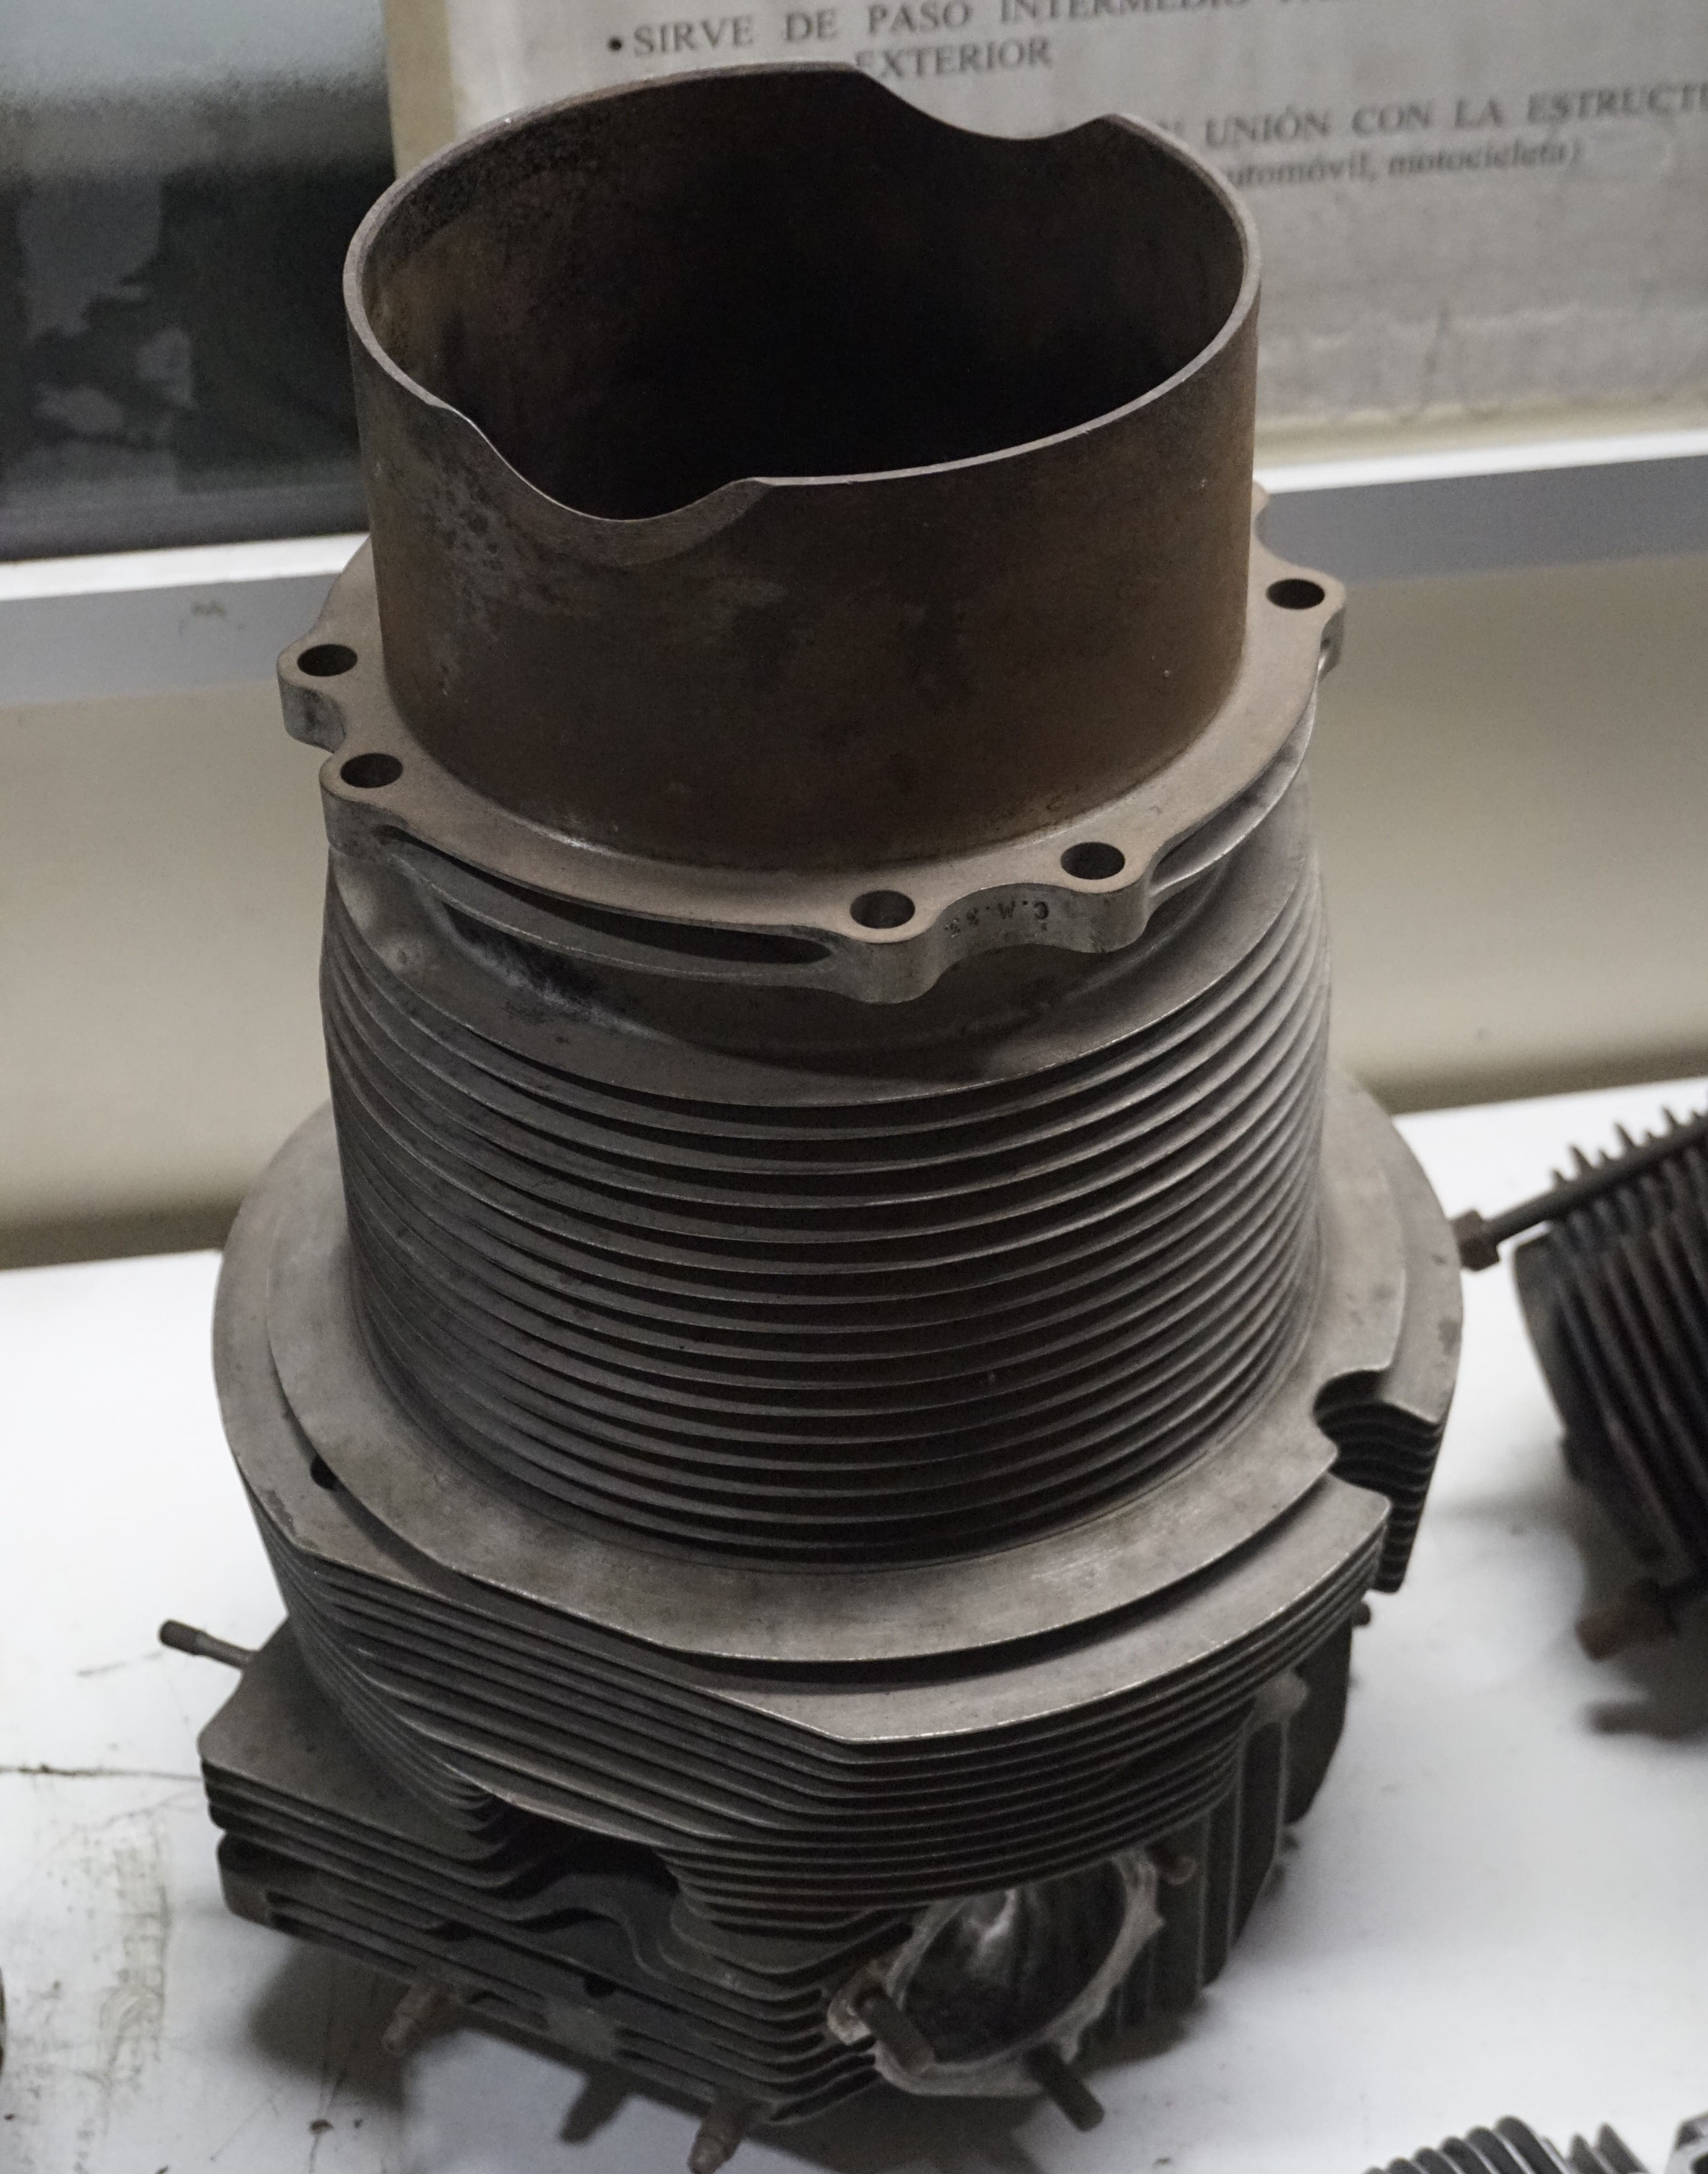
\includegraphics[width=\linewidth]{Figures/02/m3/cilindro_radial.jpg}
		\caption{Cilindro de motor radial.}
		\label{fig:bloq_bmw}
	\end{subfigure}
	\hfill
	\begin{subfigure}[b]{0.45\textwidth}
 		\centering
 		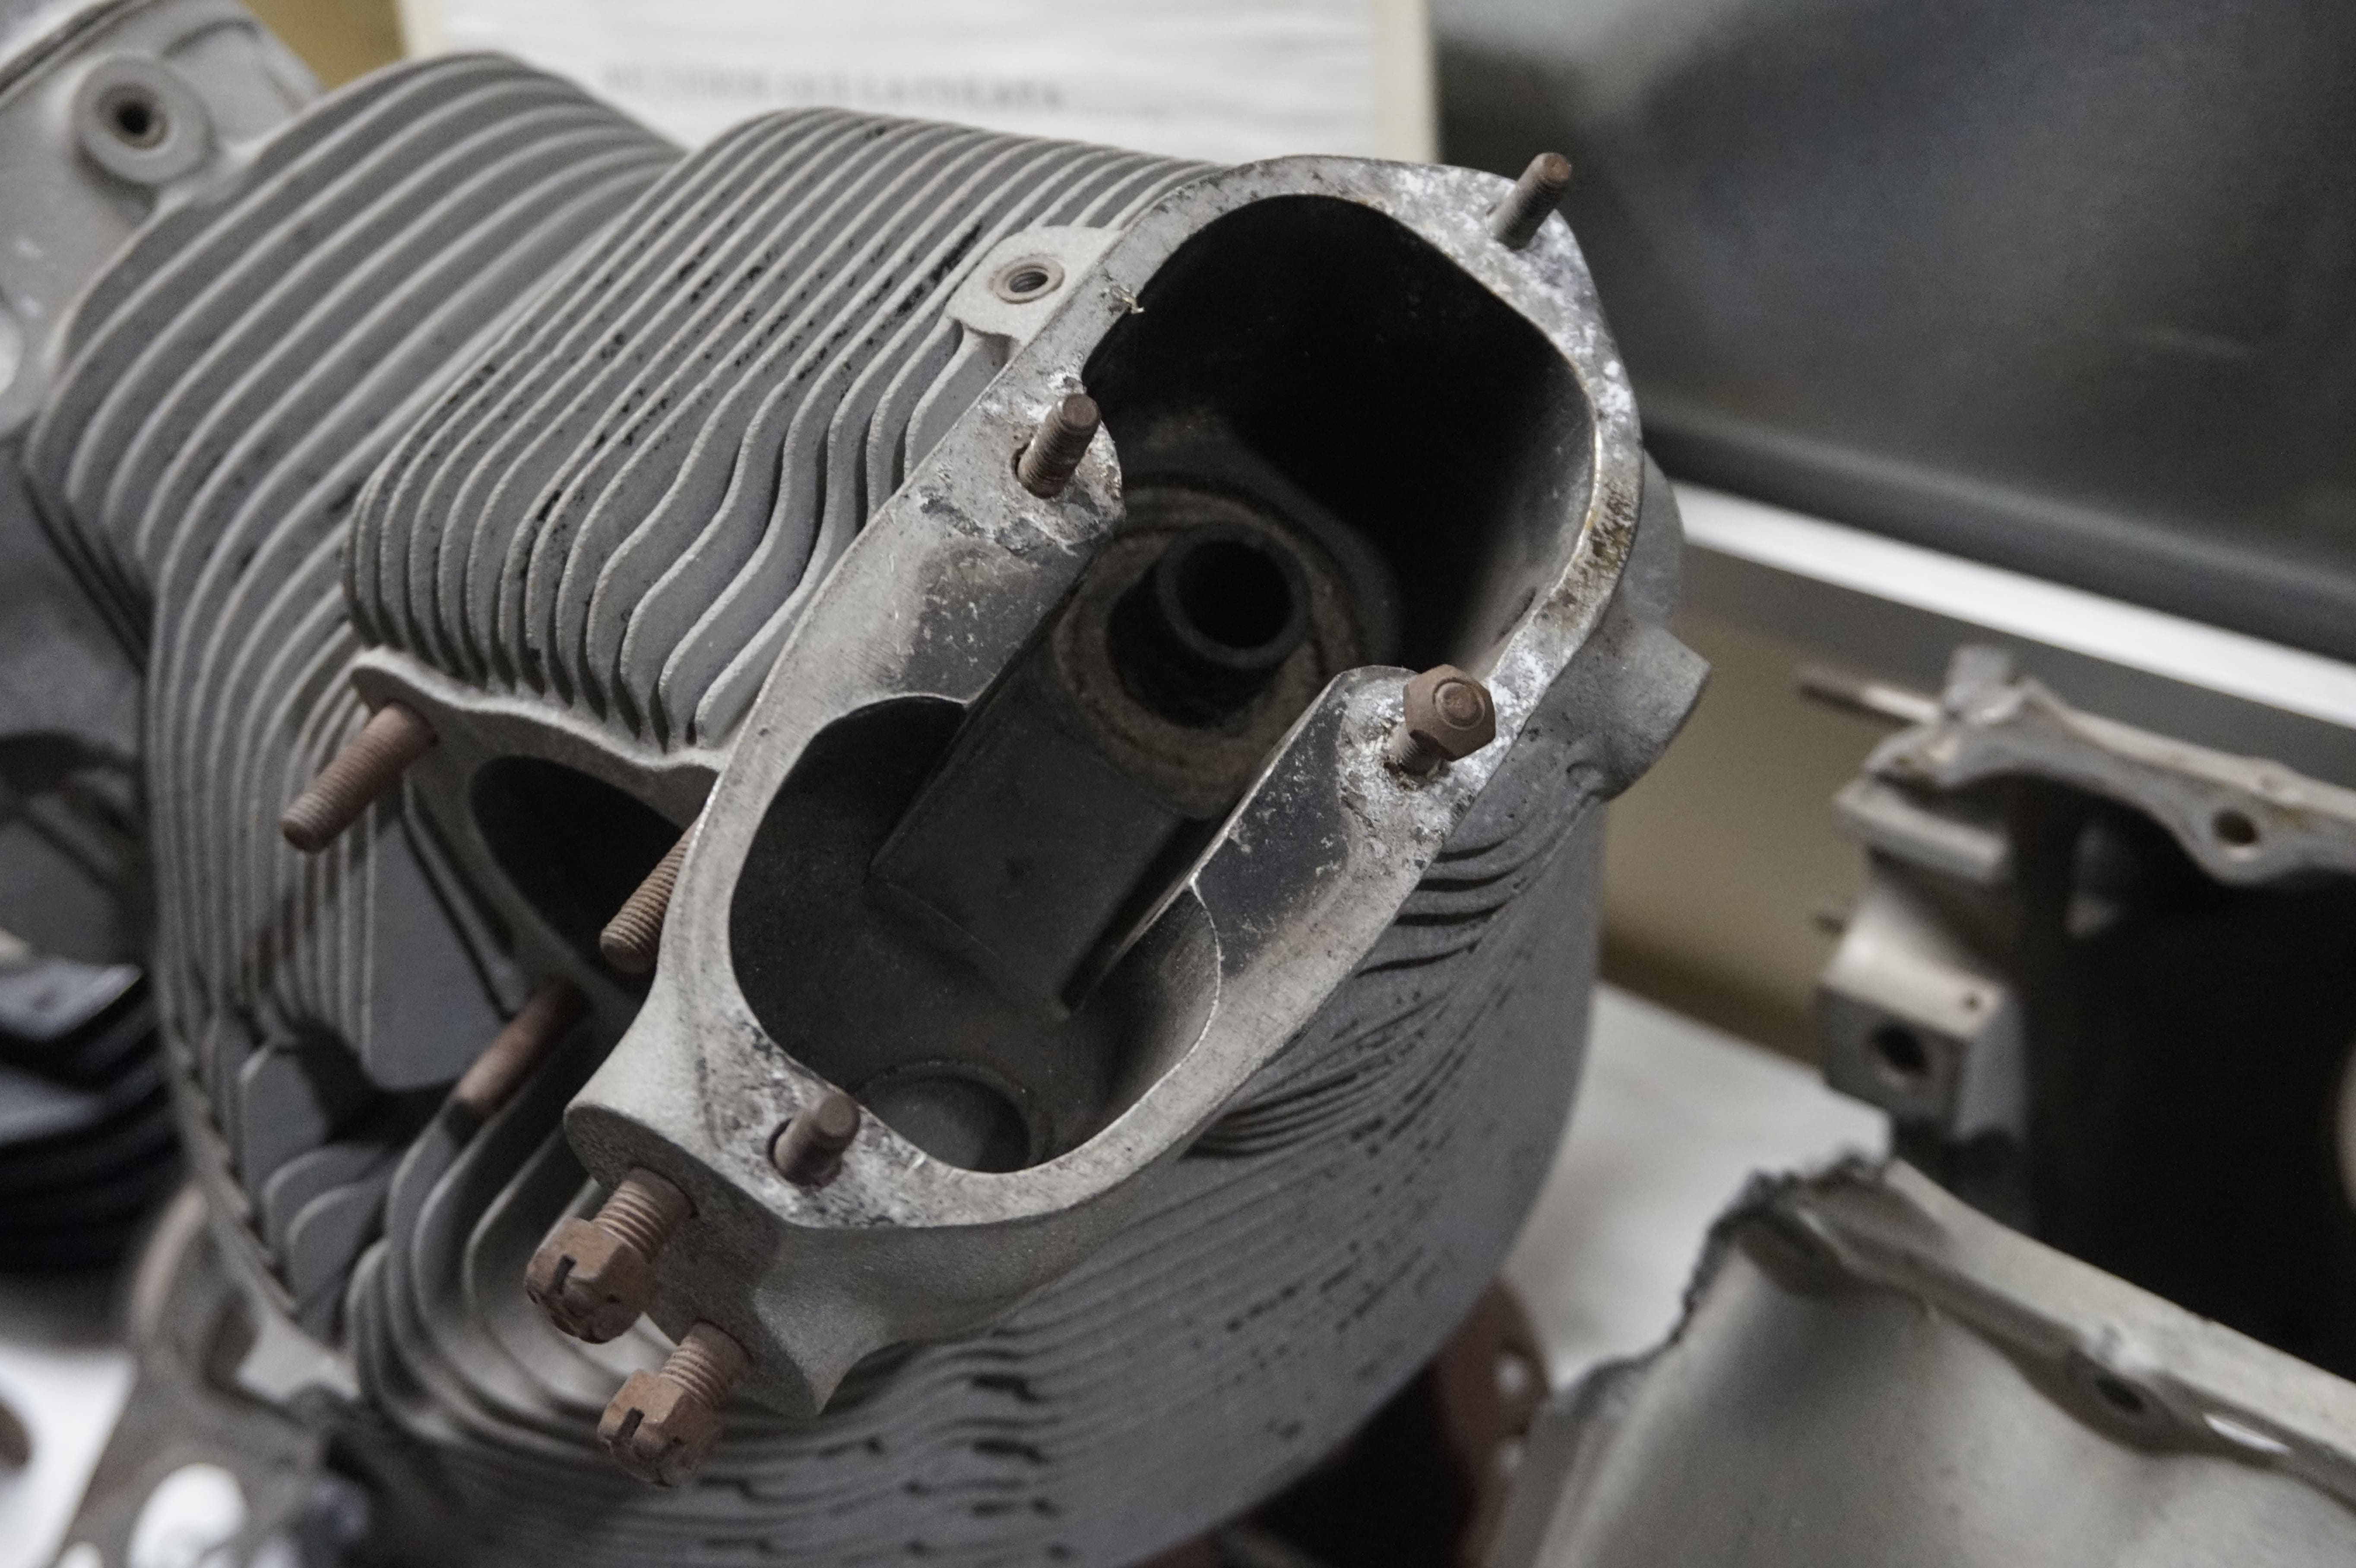
\includegraphics[width=\linewidth]{Figures/02/m3/head_radial.jpg}
 		\caption{Alojamiento del balancín.}
		\label{fig:bloq_cig}
	\end{subfigure}    
	\caption{Motor radial.}
	\label{fig:block_radial}
\end{figure}

\newpage

\section{Cigüeñal y Biela} \label{s:secion_04}

En la presente sección se discutirán los elementos encargados de transmitir el trabajo que realizan los pistones hacia el exterior del motor, los cuales también se encargan de convertir el movimiento alternativo de dichos pistones en un movimiento continuo de rotación. Al ser elementos muy exigidos mecánicamente (tanto por las cargas generadas por las presiones en el pistón como por aquellas provocadas por la inercia) son habitualmente fabricados en aleaciones de acero, y en muchos casos se trata de elementos que son forjados para mejorar sus características mecánicas.

\subsection{Cigüeñal} \label{ss:crankshaft}

El cigüeñal es el elemento al que se acoplan las bielas (discutidas en el apartado \ref{ss:conrod}) a lo largo de él, y en cuyo extremo se instala habitualmente el volante de inercia. En función de la distancia entre los ejes de los cilindros, y de las cargas que se espera que soporte el cigüeñal, este mismo tendrá una cantidad mayor o menor de apoyos. Se observa en la figura \ref{fig:cigs} que uno de los dos cigüeñales tiene únicamente tres apoyos (se trata de una pieza de un motor de cilindros opuestos, por lo que los cilindros no interfieren entre sí dos a dos), mientras que el otro presenta cinco apoyos (al ser de un motor en línea, las muñequillas han de estar más separadas entre sí para evitar la interferencia entre cilindros).

\begin{figure}[H]
	\centering
	\begin{subfigure}[b]{0.45\textwidth}
		\centering
		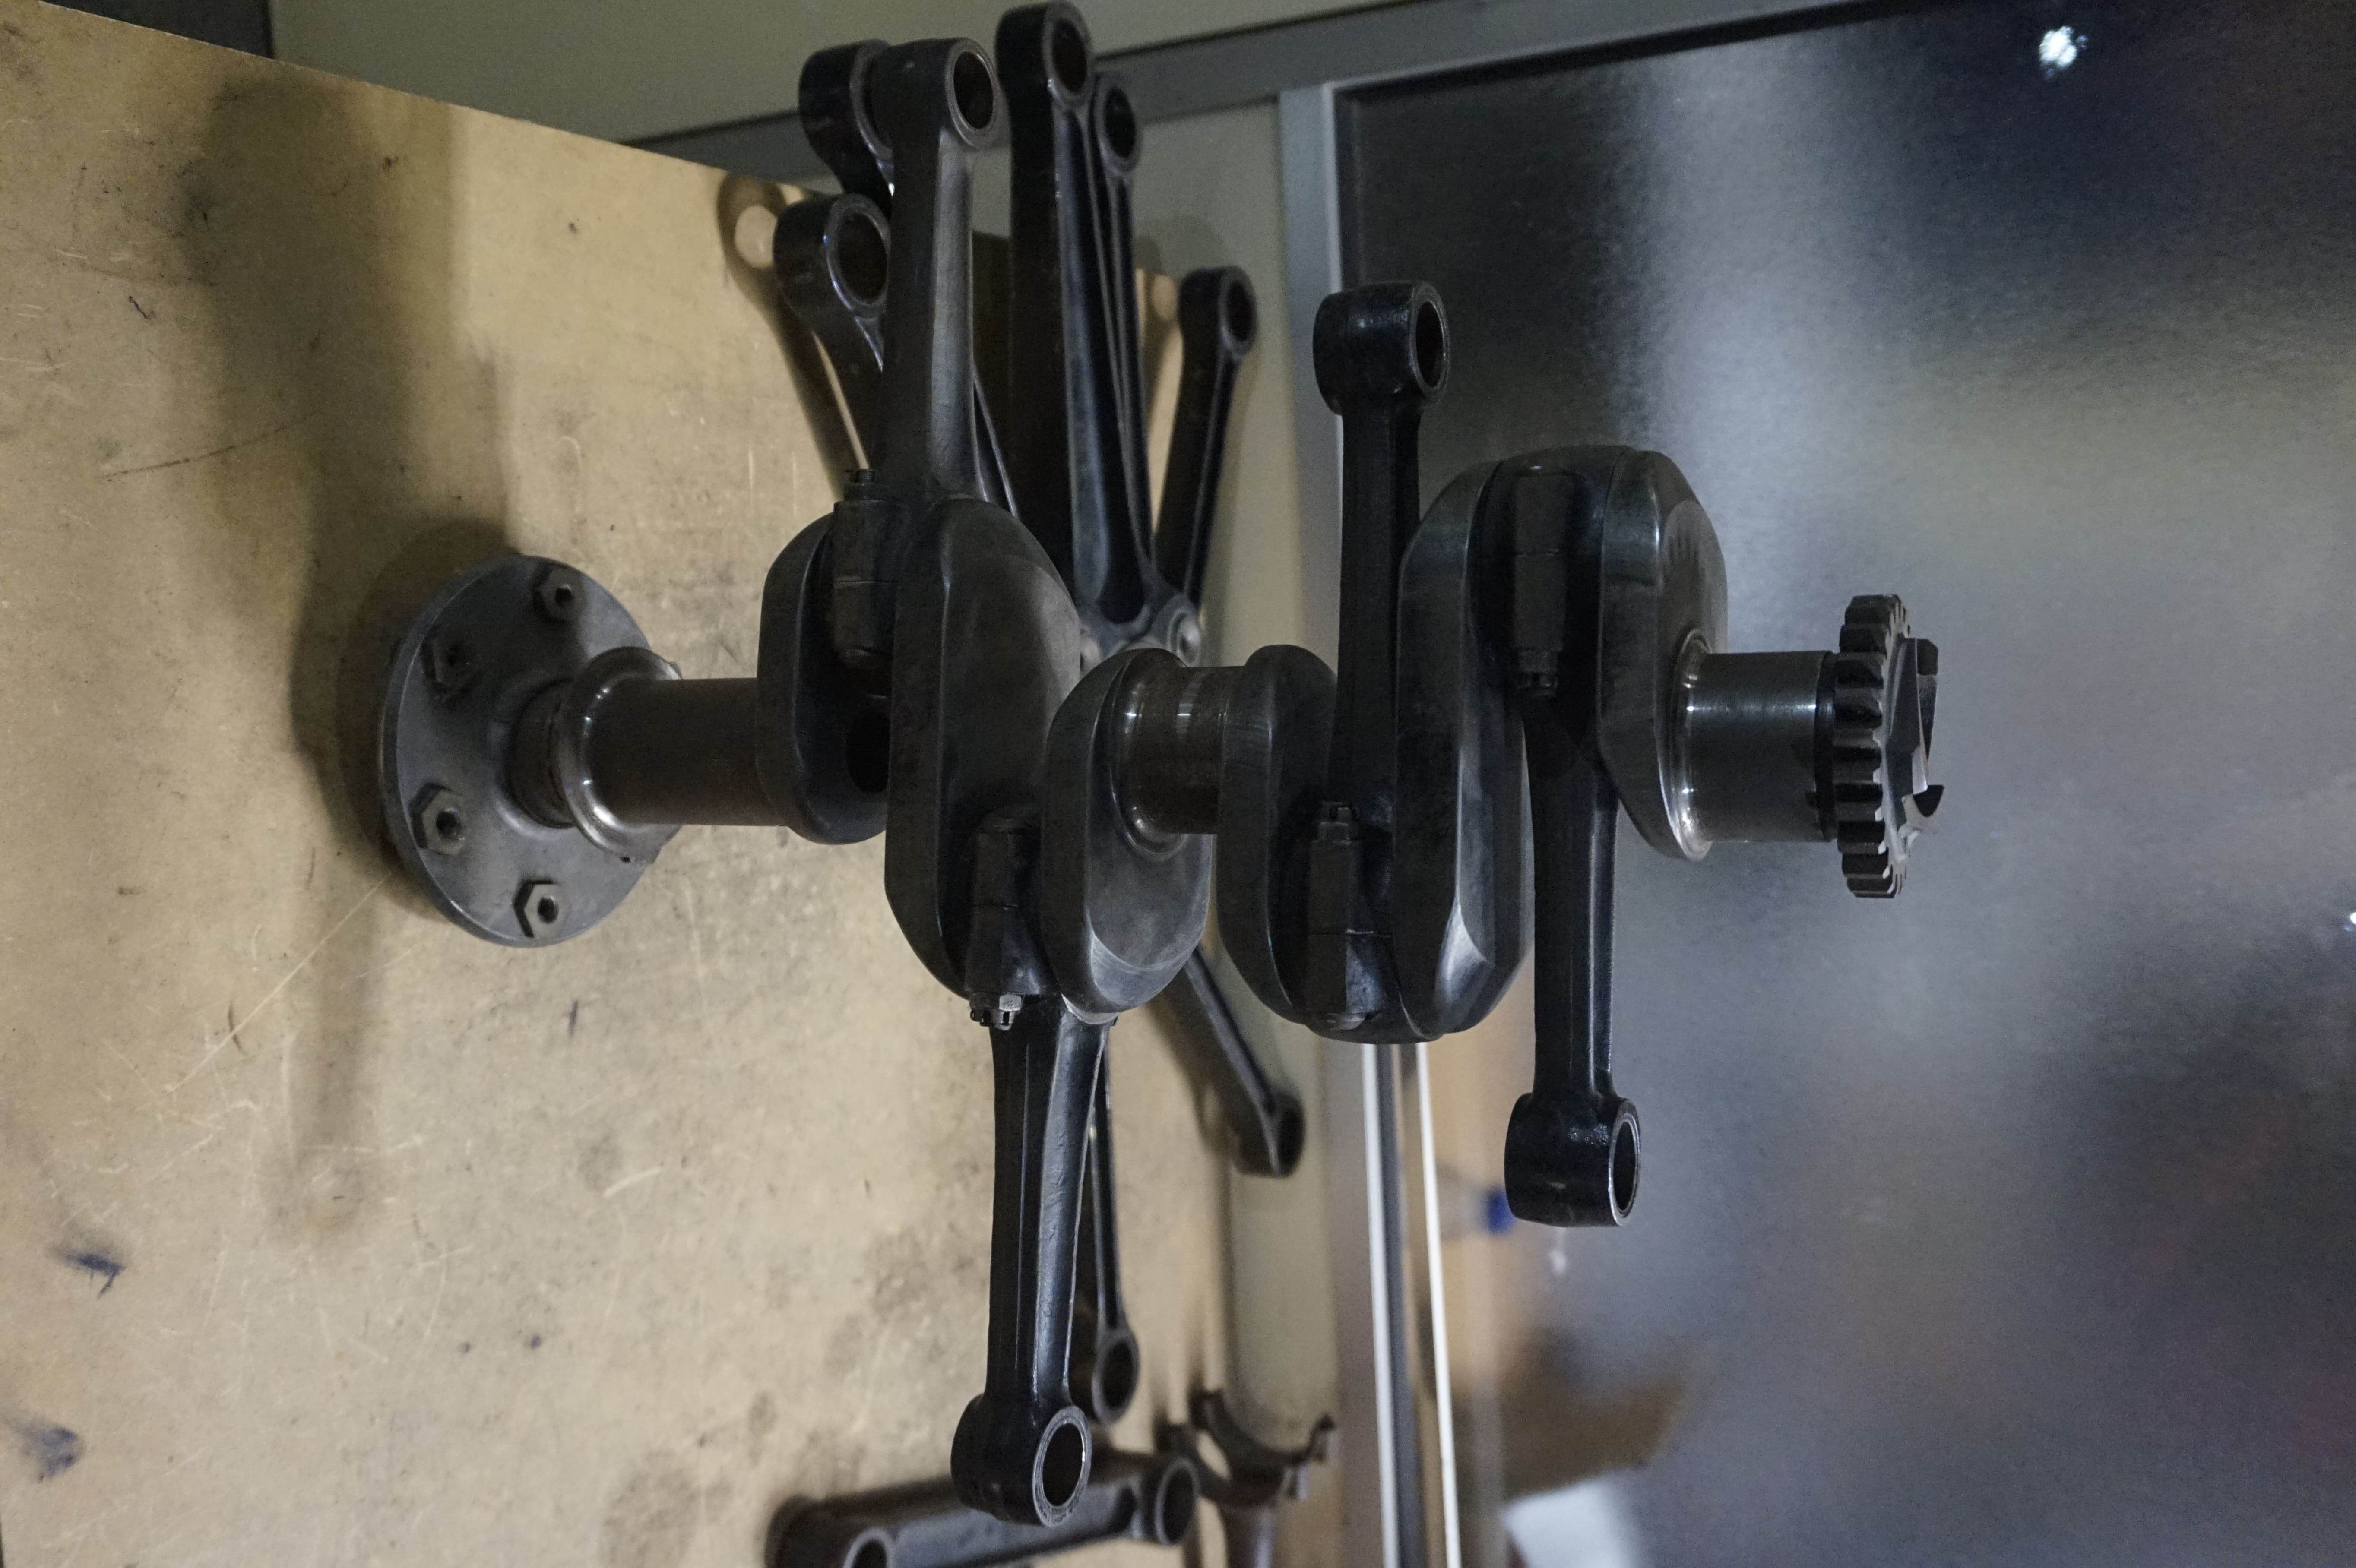
\includegraphics[width=\linewidth]{Figures/02/m4/cig_boxer.jpg}
		\caption{Motor bóxer de aviación.}
		\label{fig:box_cig}
	\end{subfigure}
	\hfill
	\begin{subfigure}[b]{0.45\textwidth}
 		\centering
 		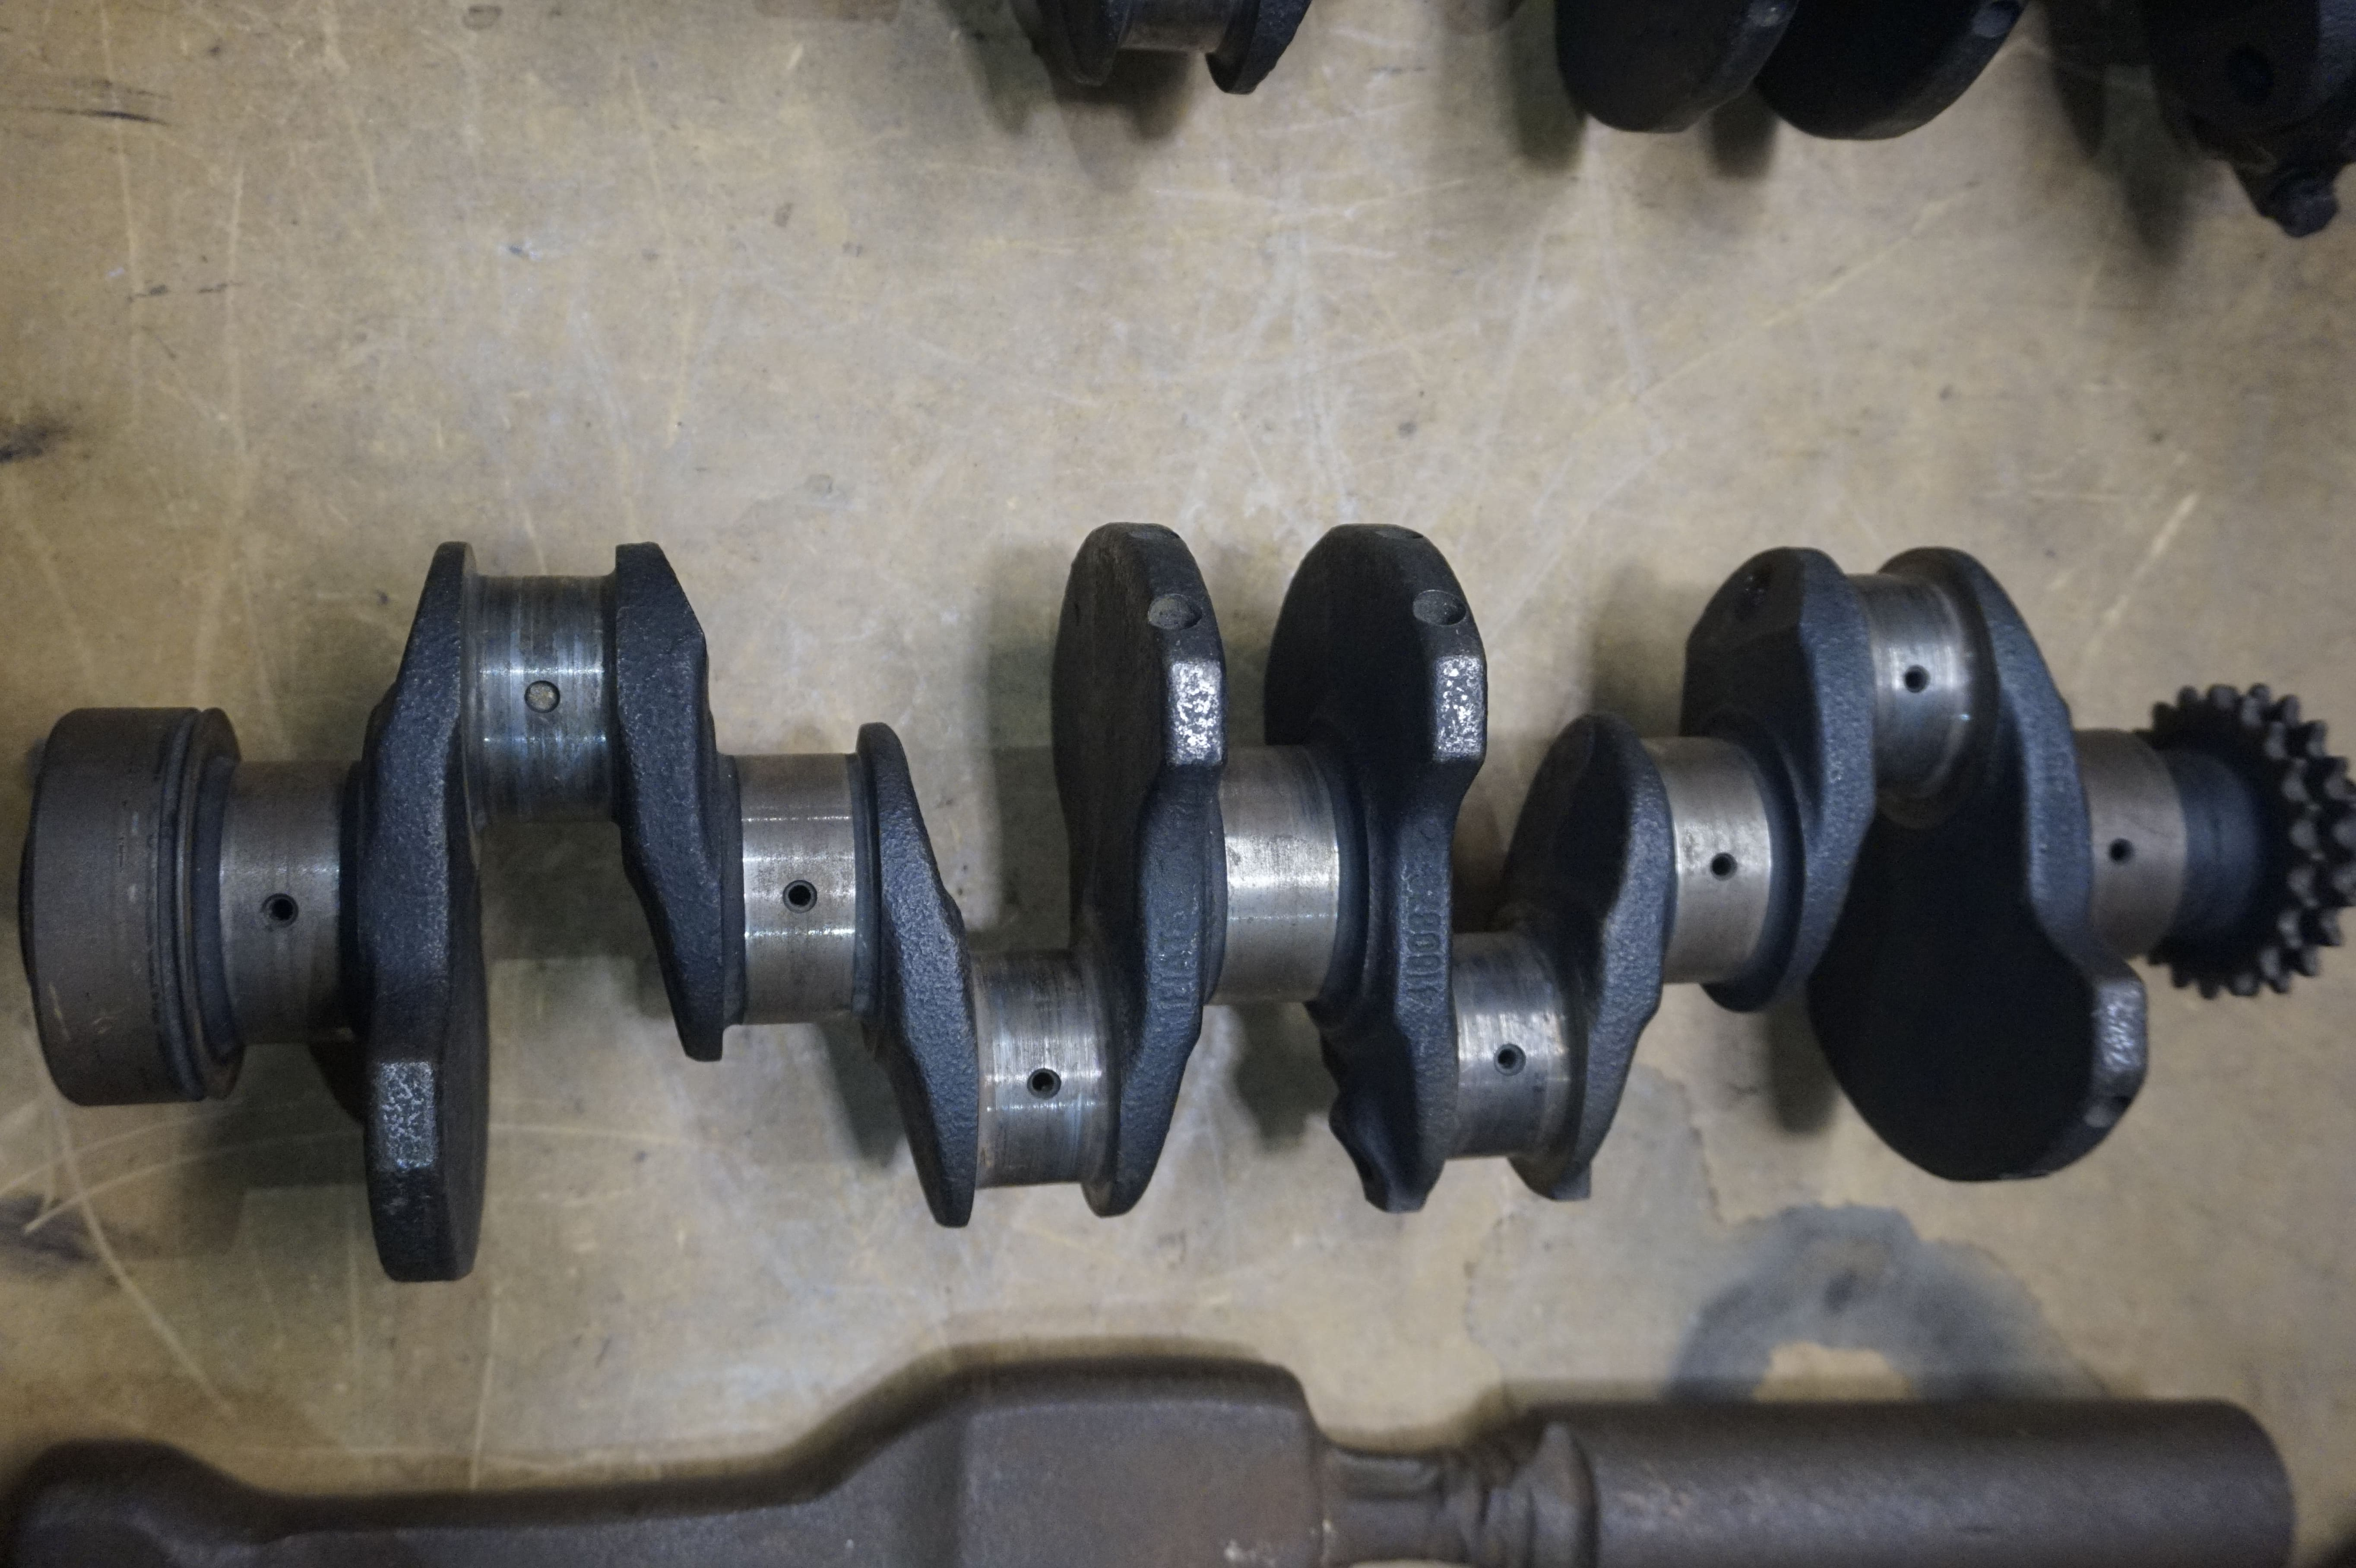
\includegraphics[width=\linewidth]{Figures/02/m4/cig_I4.jpg}
 		\caption{Motor I4.}
		\label{fig:cig_I4}
	\end{subfigure}    
	\caption{Cigüeñales.}
	\label{fig:cigs}
\end{figure}

Dado que los cigüeñales no son simétricos, muchos de ellos (como el de la figura \ref{fig:cig_I4} han de llevar contrapesos en los lugares opuestos a las muñequillas, para disminuir las vibraciones (y las cargas) a las que se ve sometido el conjunto de piezas que forman el motor. Para equilibrar el cigüeñal se practican agujeros en los contrapesos (que no en las zonas cilíndricas del mismo), de manera que se va retirando material de dichos contrapesos hasta que queda el cigüeñal correctamente equilibrado.\\

Dado que los cigüeñales tienen velocidades de rotación del orden de los miles de revoluciones por minuto, el rozamiento en los apoyos y las muñequillas es de gran importancia, y ha de minimizarse, lo que se consigue mediante cojinetes sólidos, ayudados por una fina película de aceite a muy alta presión. El aceite es suministrado a las muñequillas a través del propio cigüeñal, mediante los agujeros visibles en las mismas. El suministro de aceite al cigüeñal, se hace a través de los agujeros practicados en los apoyos que van alojados en el bloque motor.


\subsection{Bielas} \label{ss:conrod}

Las bielas son los elementos más exigidos mecánicamente de todo el motor, pues han de soportar a compresión las cargas de presión generadas por los pistones, y a tracción, la fuerza que hace el cigüeñal con objetivo de llenar el pistón en el tiempo de admisión. Por ello, se fabrican en aleaciones de acero de forja, mediante un proceso de estampación y posterior mecanizado. En la figura \ref{fig:wrought} se observan las distintas fases por las que pasa la biela en su proceso de fabricación, desde la barra de metal desde la que se obtendrá la pieza, hasta que se le practica el agujero para unirla al cigüeñal, pero antes de realizar el corte que permite finalmente dicha operación. Finalmente la figura \ref{fig:conrod} es una fotografía de una biela también terminada, a falta de ser separada en la parte principal y la tapa que la fija al cigüeñal.


\begin{figure}[H]
	\centering
	\begin{subfigure}[b]{0.45\textwidth}
		\centering
		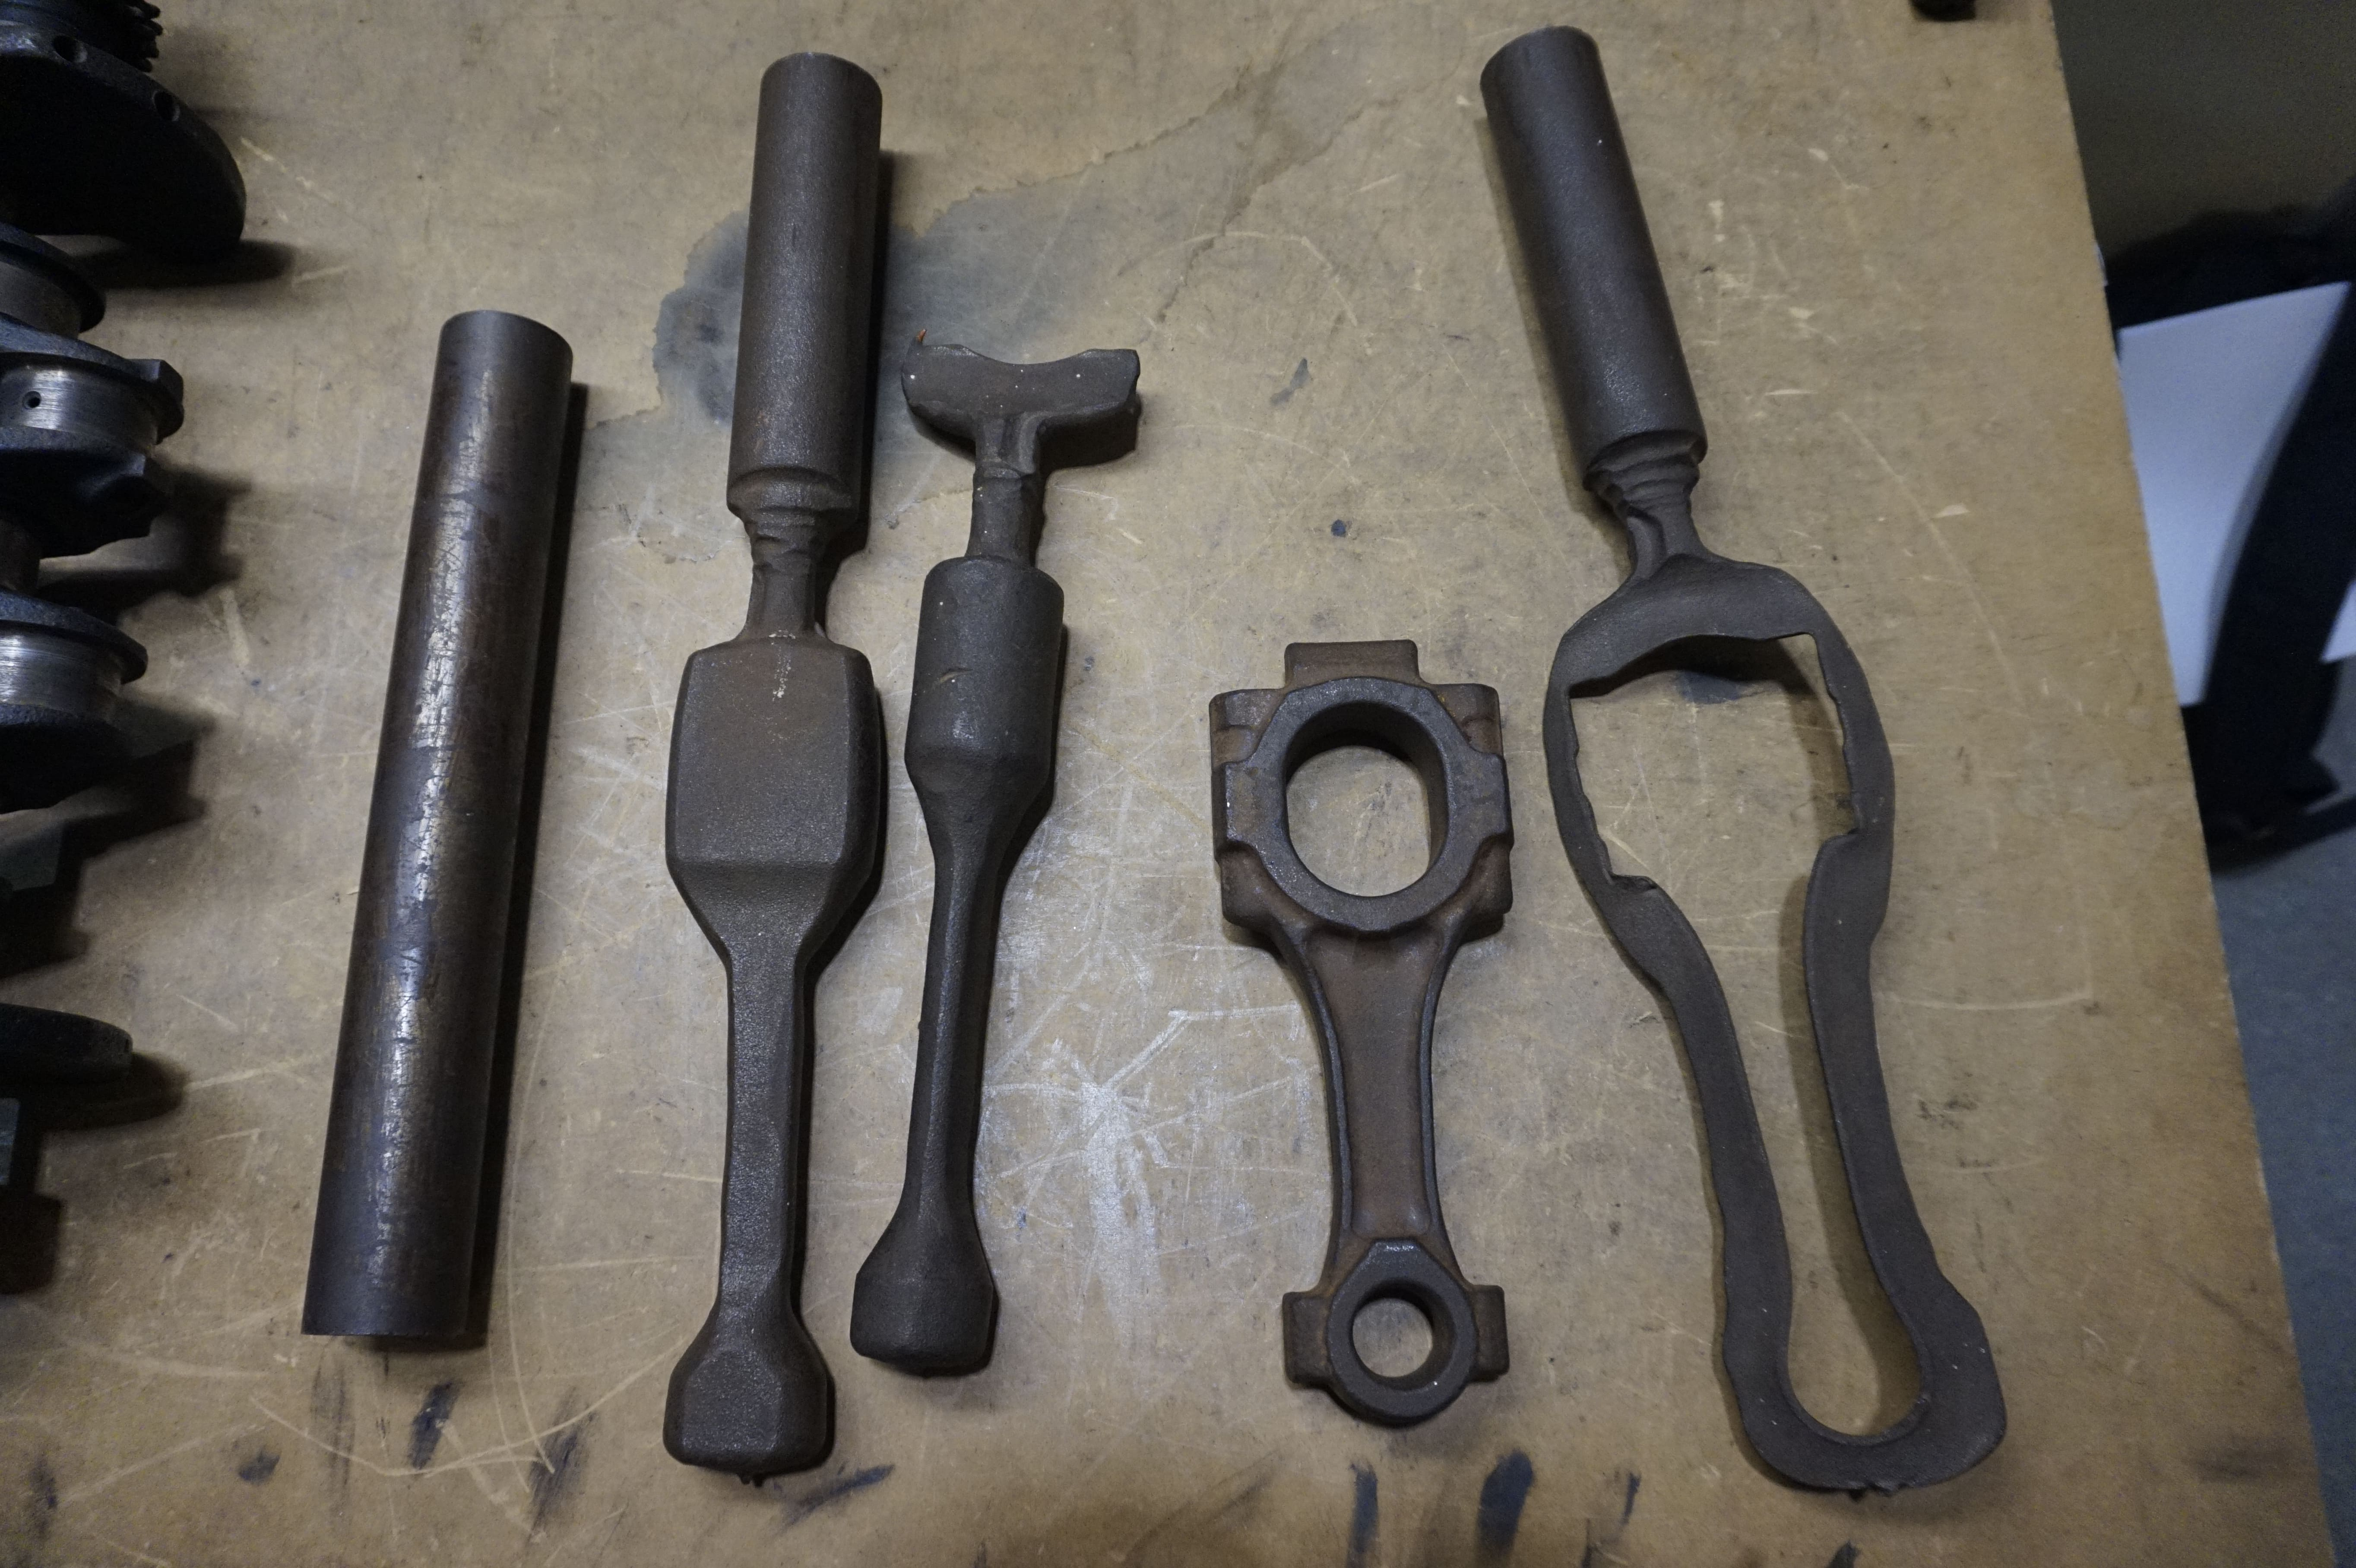
\includegraphics[width=\linewidth]{Figures/02/m4/conrod_steps.jpg}
		\caption{Proceso de producción.}
		\label{fig:forja_1}
	\end{subfigure}
	\hfill
	\begin{subfigure}[b]{0.45\textwidth}
 		\centering
 		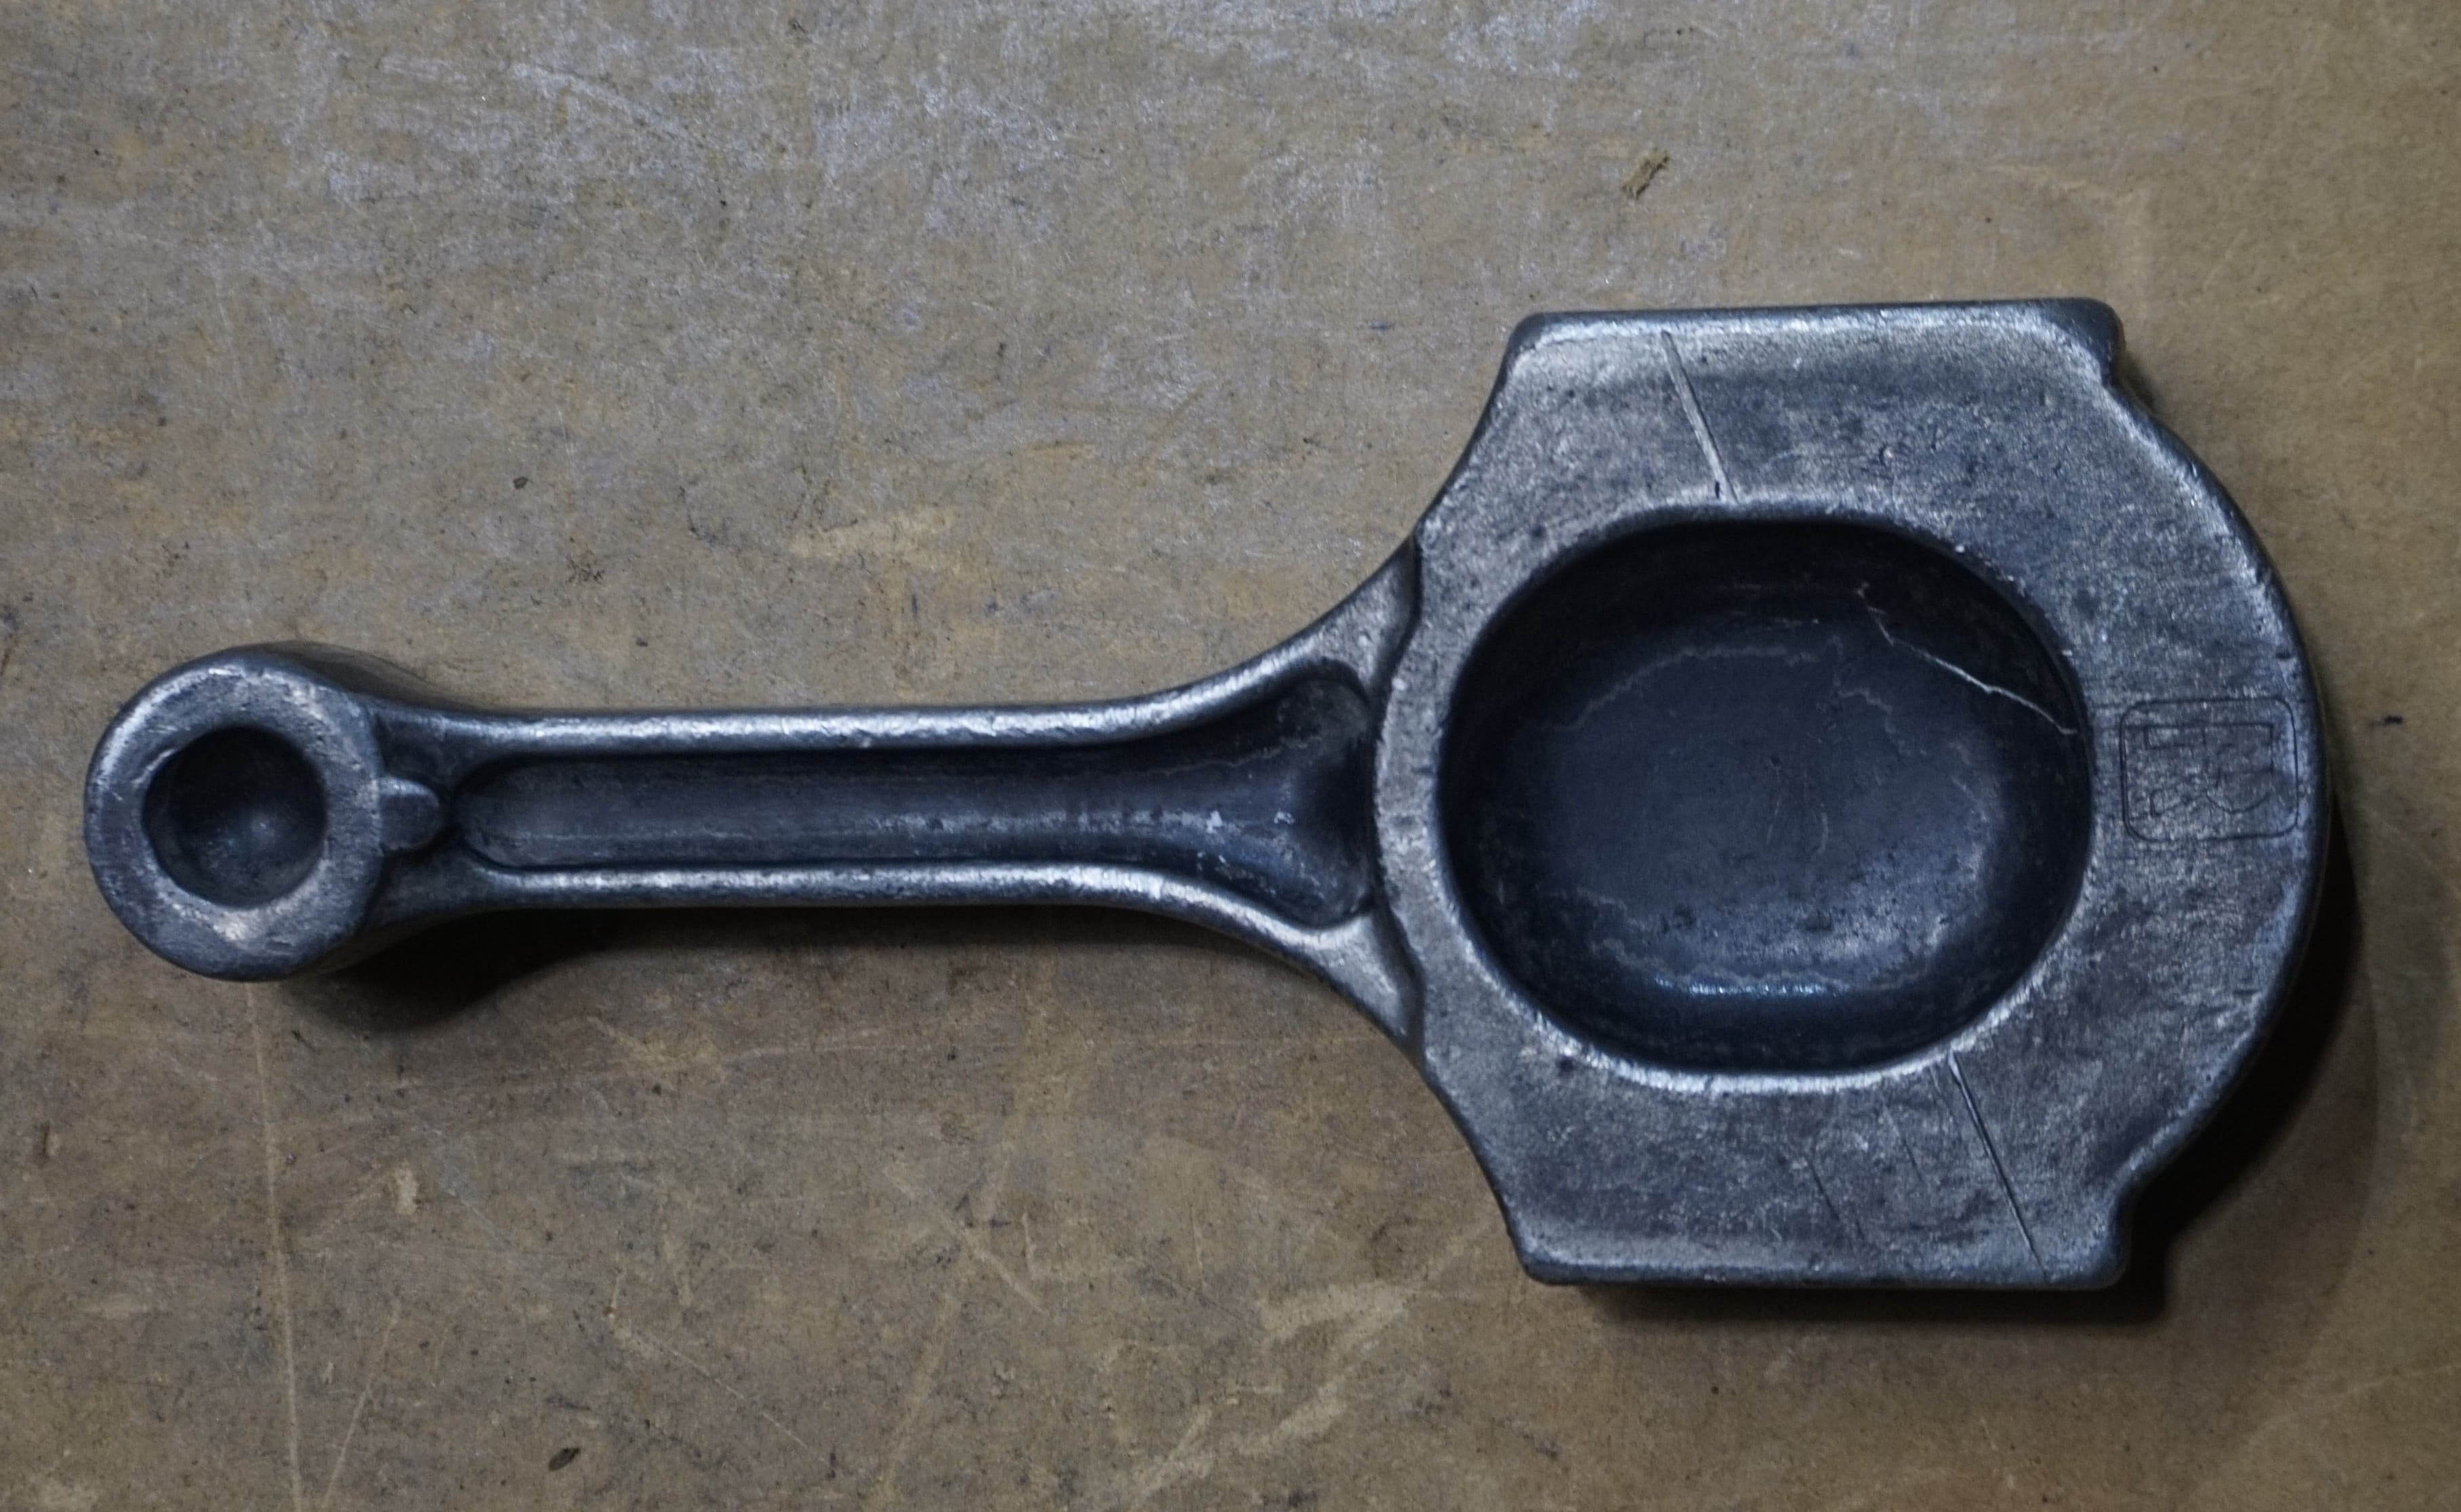
\includegraphics[width=\linewidth]{Figures/02/m4/conrod_raw.jpg}
 		\caption{Previo a ser agujerada.}
		\label{fig:forja_2}
	\end{subfigure}    
	\caption{Producción de la biela.}
	\label{fig:wrought}
\end{figure}

\begin{figure}[H]
	\centering
	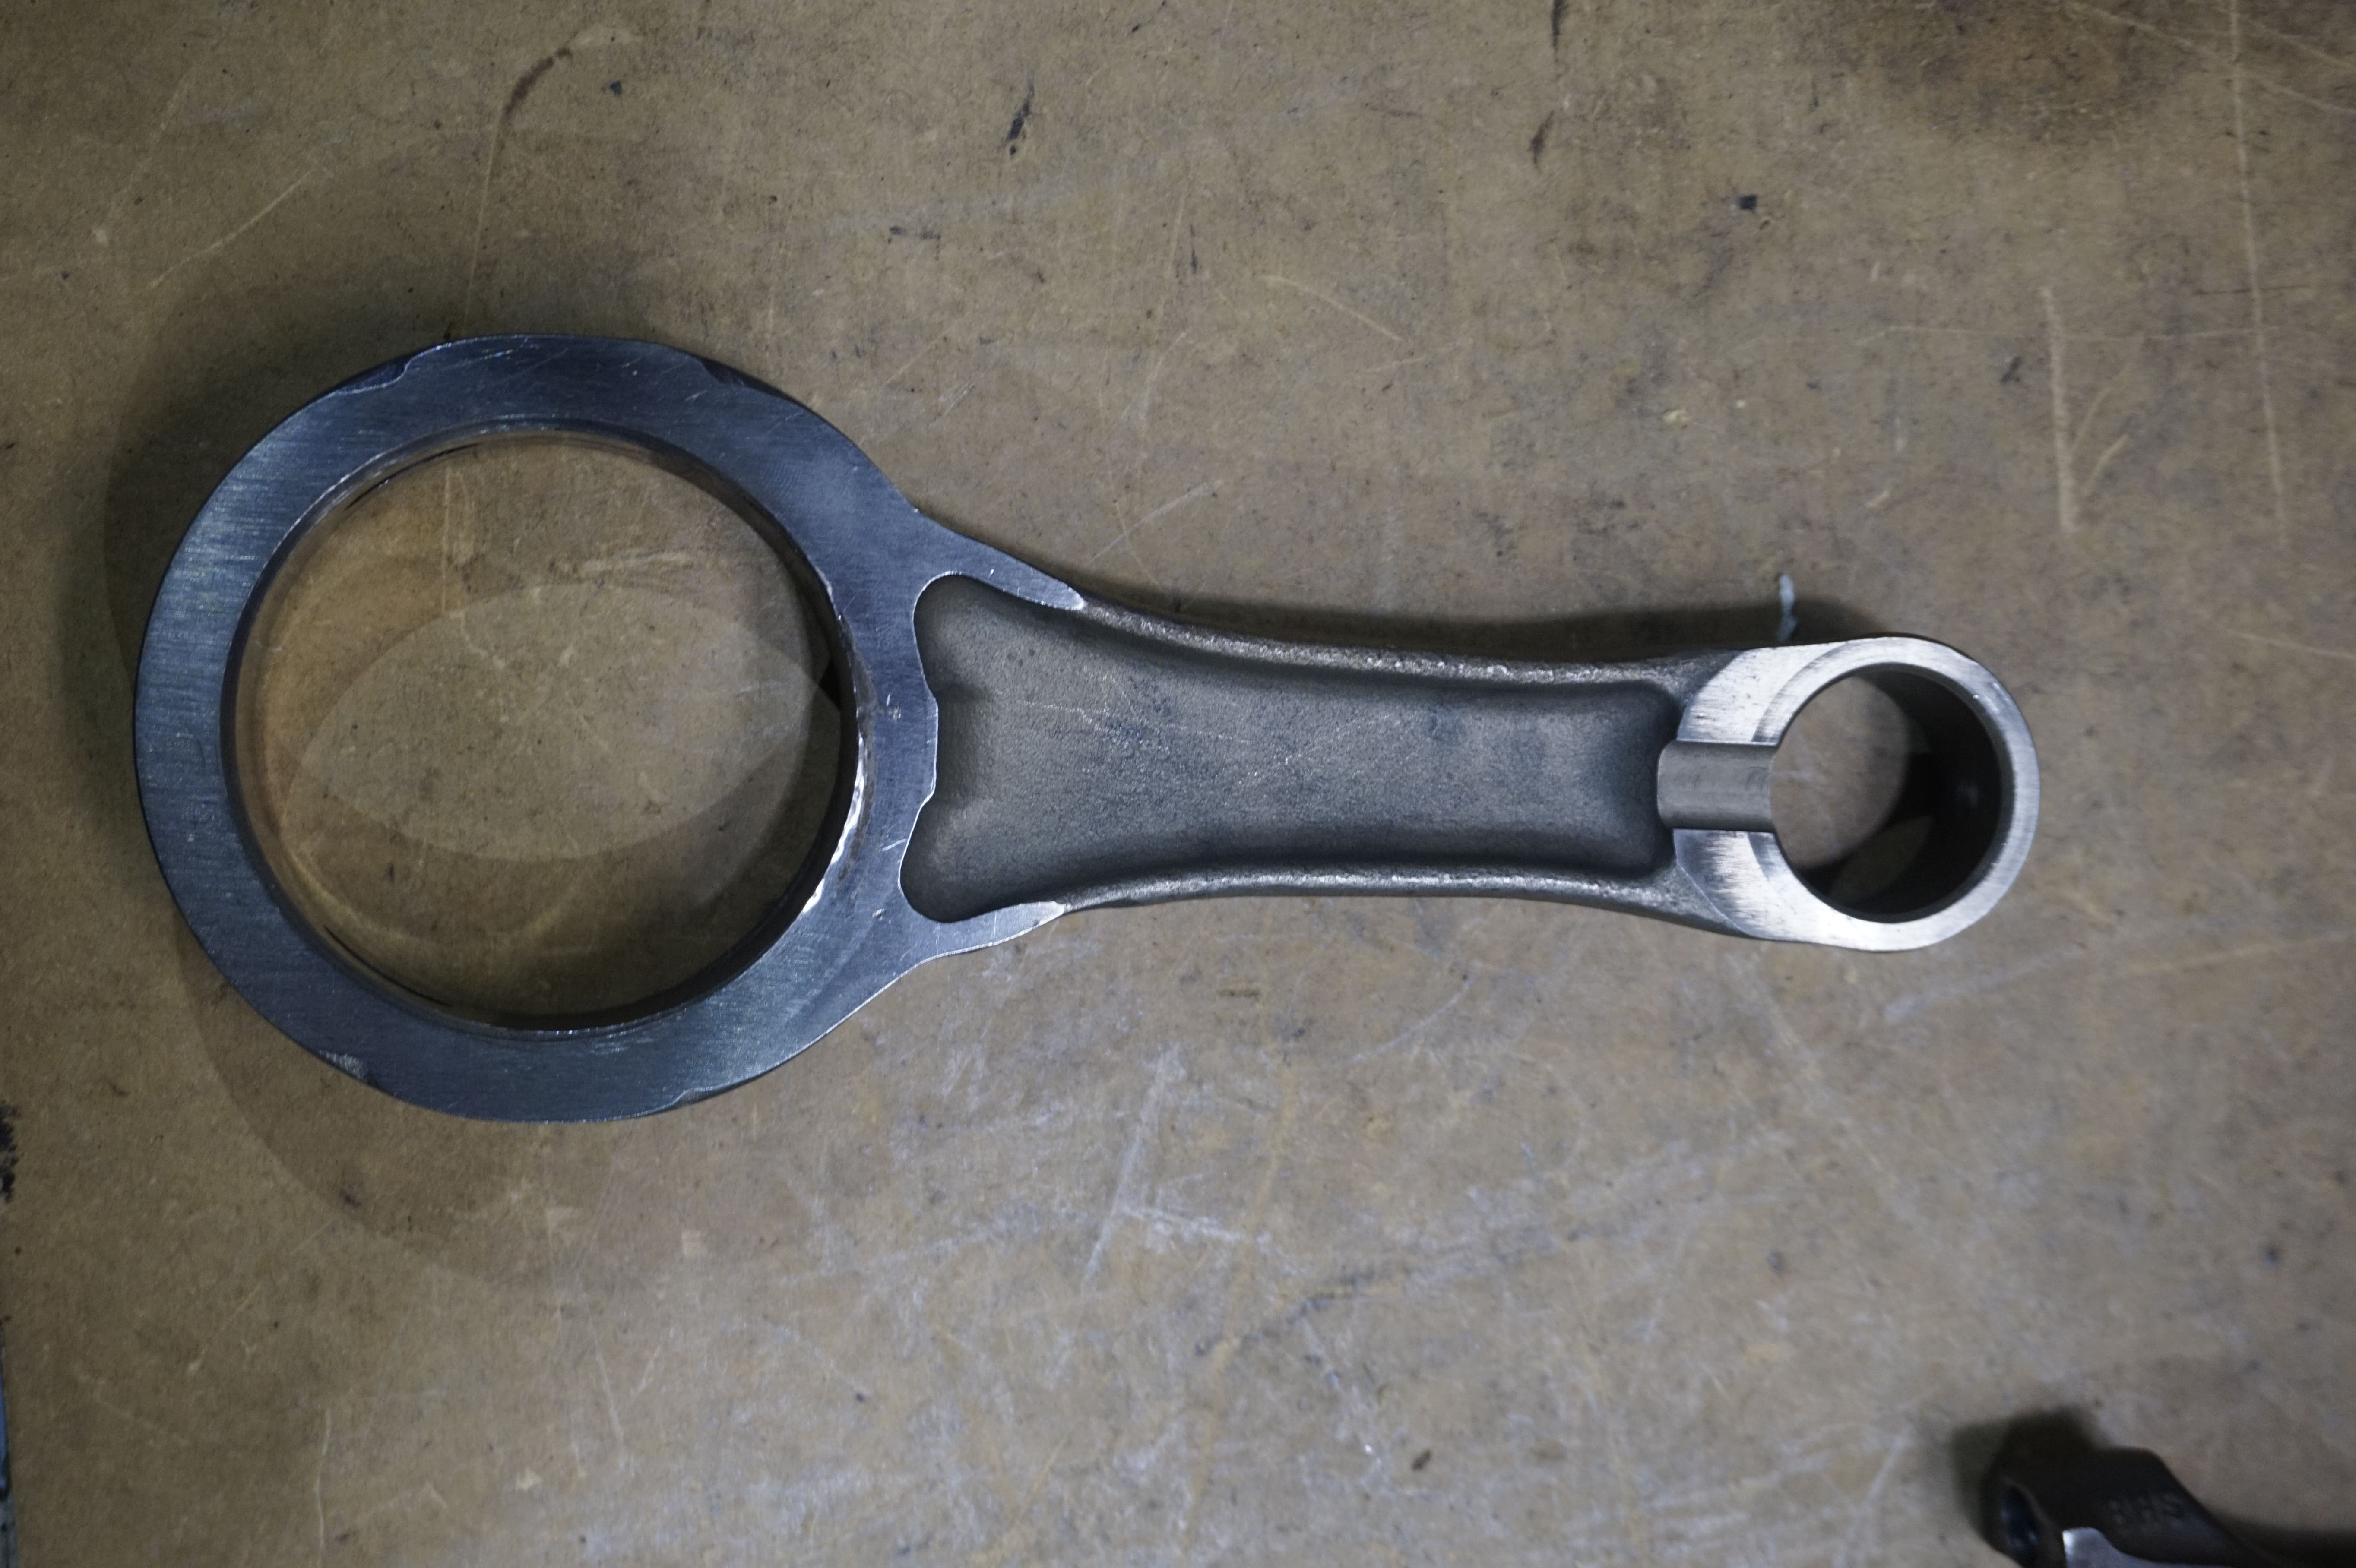
\includegraphics[width=0.6\linewidth]{Figures/02/m4/conrod.jpg}
	\caption{Biela semifinalizada.}
	\label{fig:conrod}
\end{figure}

Es interesante también observar que el fallo típico de las bielas es por pandeo, alrededor de su eje de mayor inercia perpendicular a la carga, pues el eje de menor inercia tiene su giro restringido al estar anclado al cigüeñal. En la figura \ref{fig:broken_conrod} se observan dos bielas sin su parte inferior que han sufrido el tipo de fallo mencionado.

\begin{figure}[H]
	\centering
	\begin{subfigure}[b]{0.45\textwidth}
		\centering
		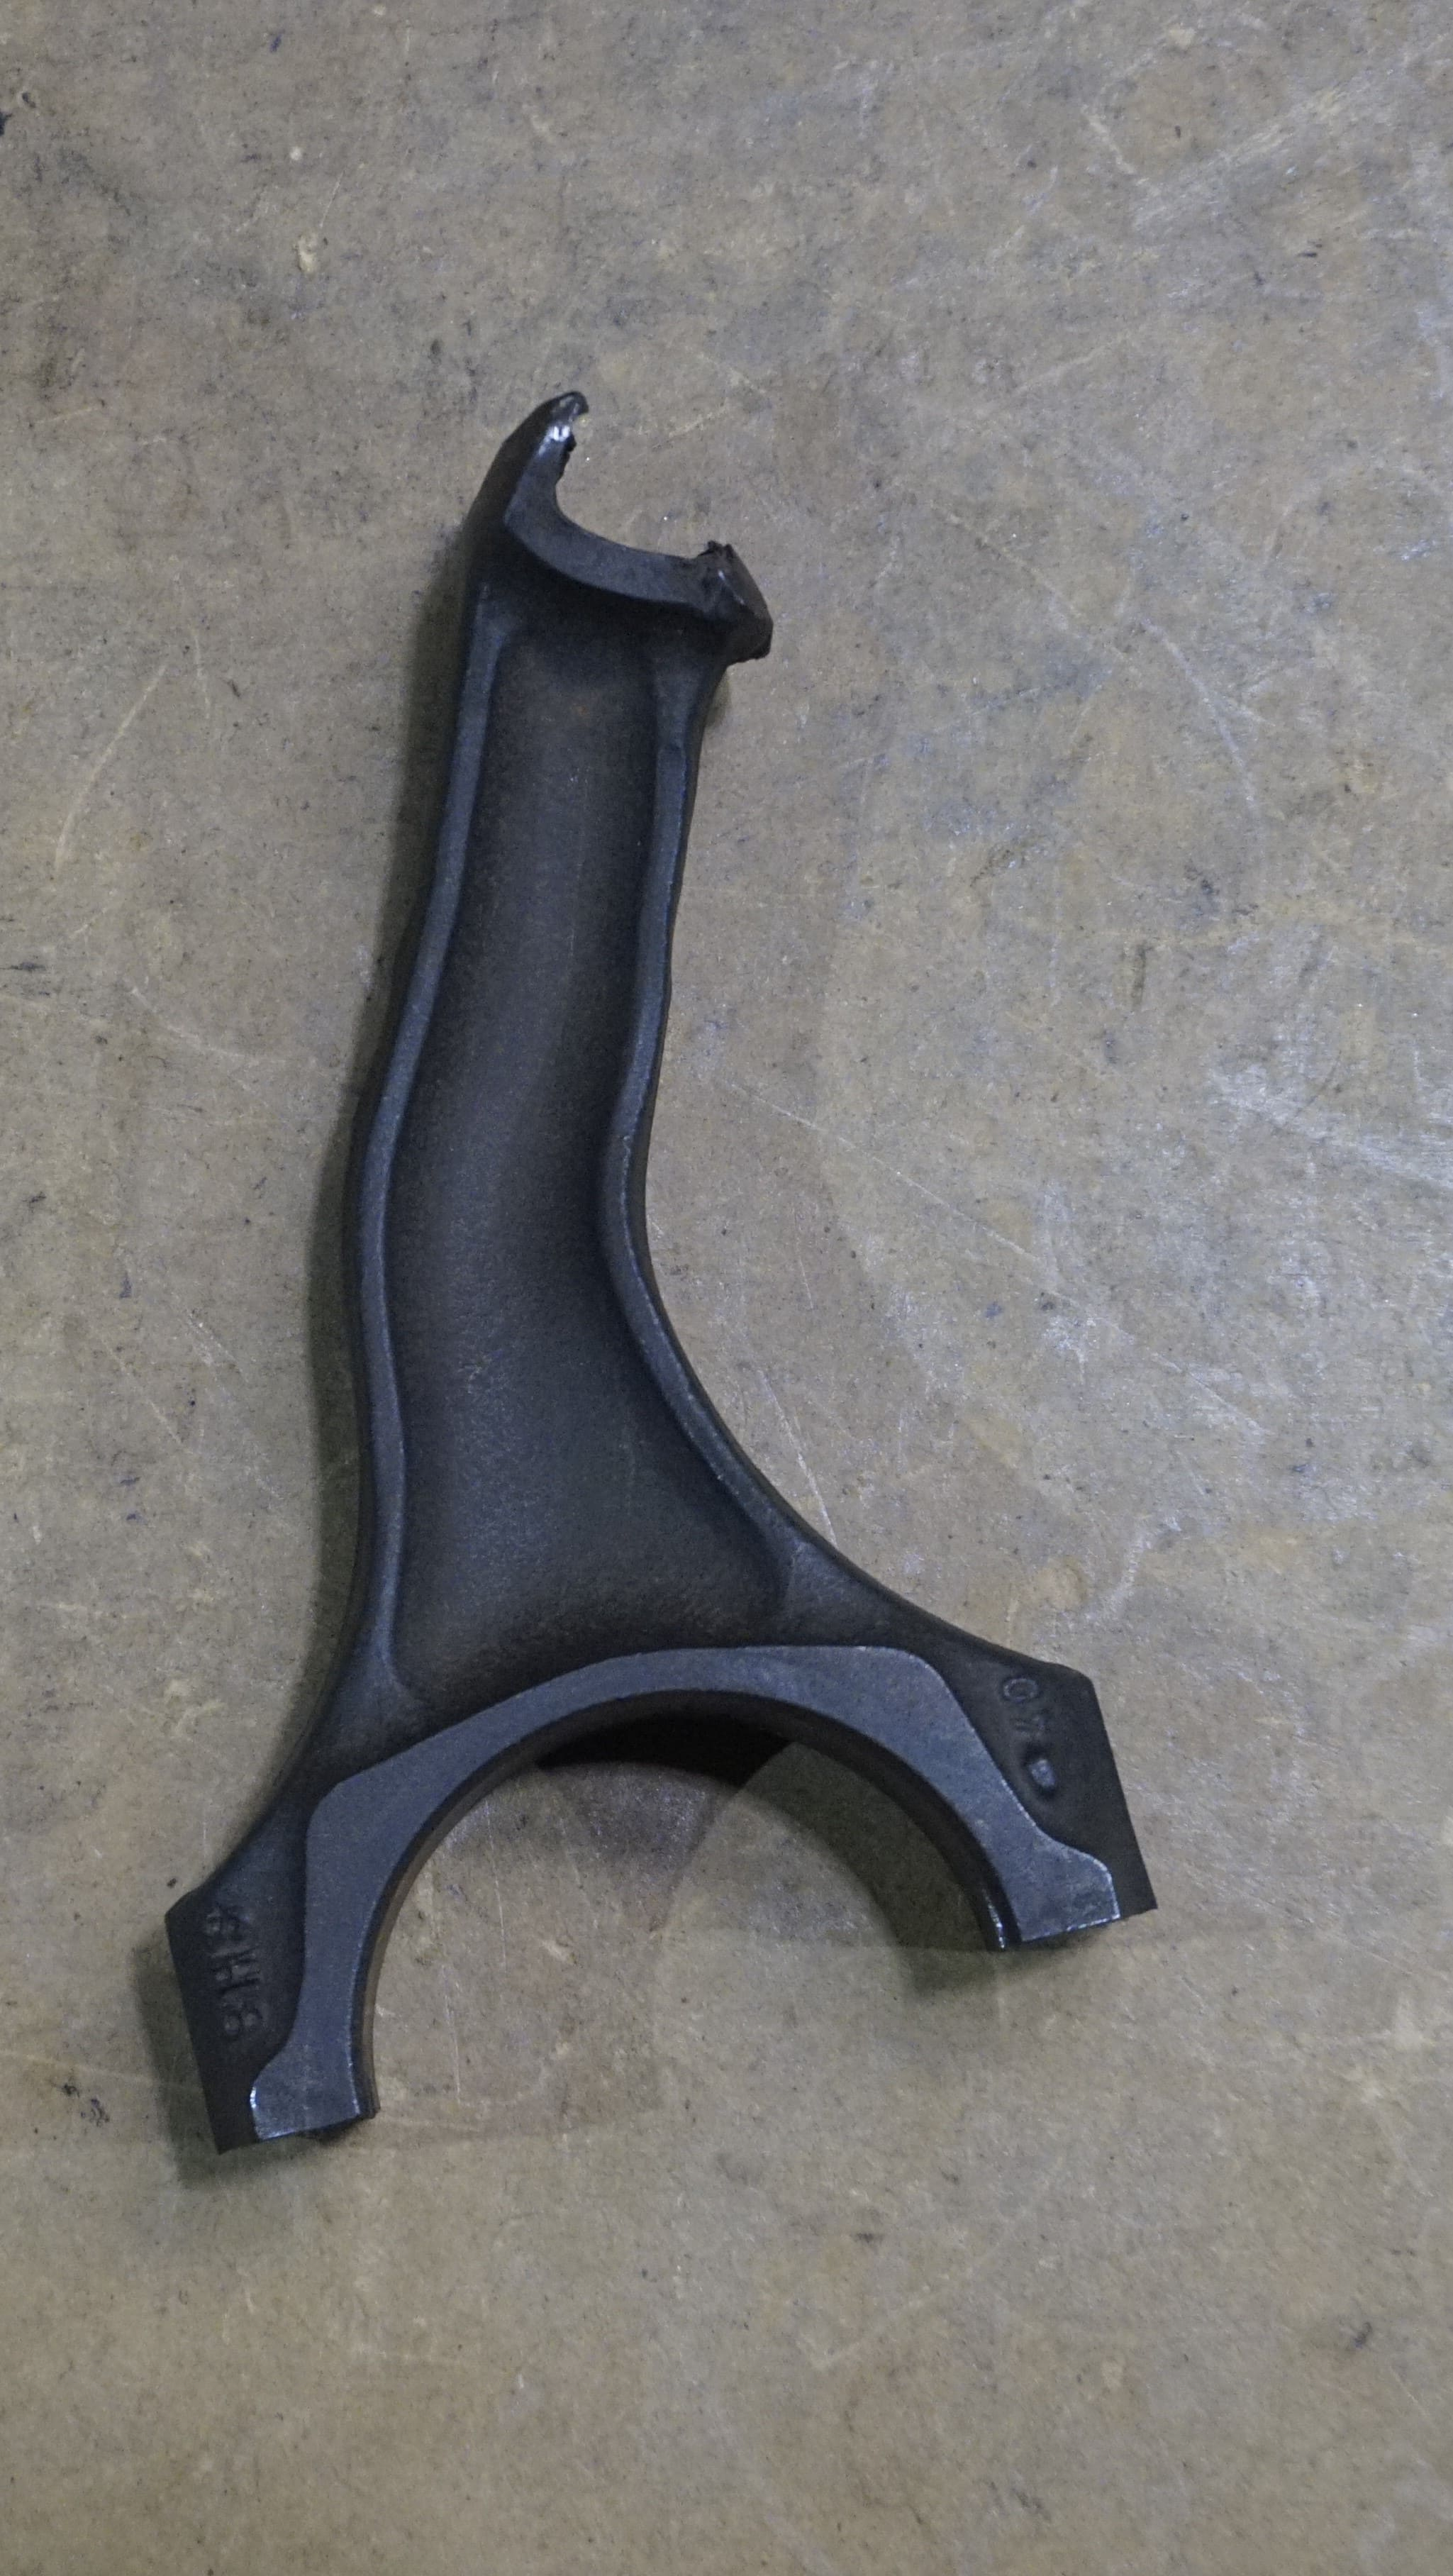
\includegraphics[width=\linewidth]{Figures/02/m4/conrod_bent.jpg}
		\caption{Biela destruida.}
		\label{fig:broken}
	\end{subfigure}
	\hfill
	\begin{subfigure}[b]{0.45\textwidth}
 		\centering
 		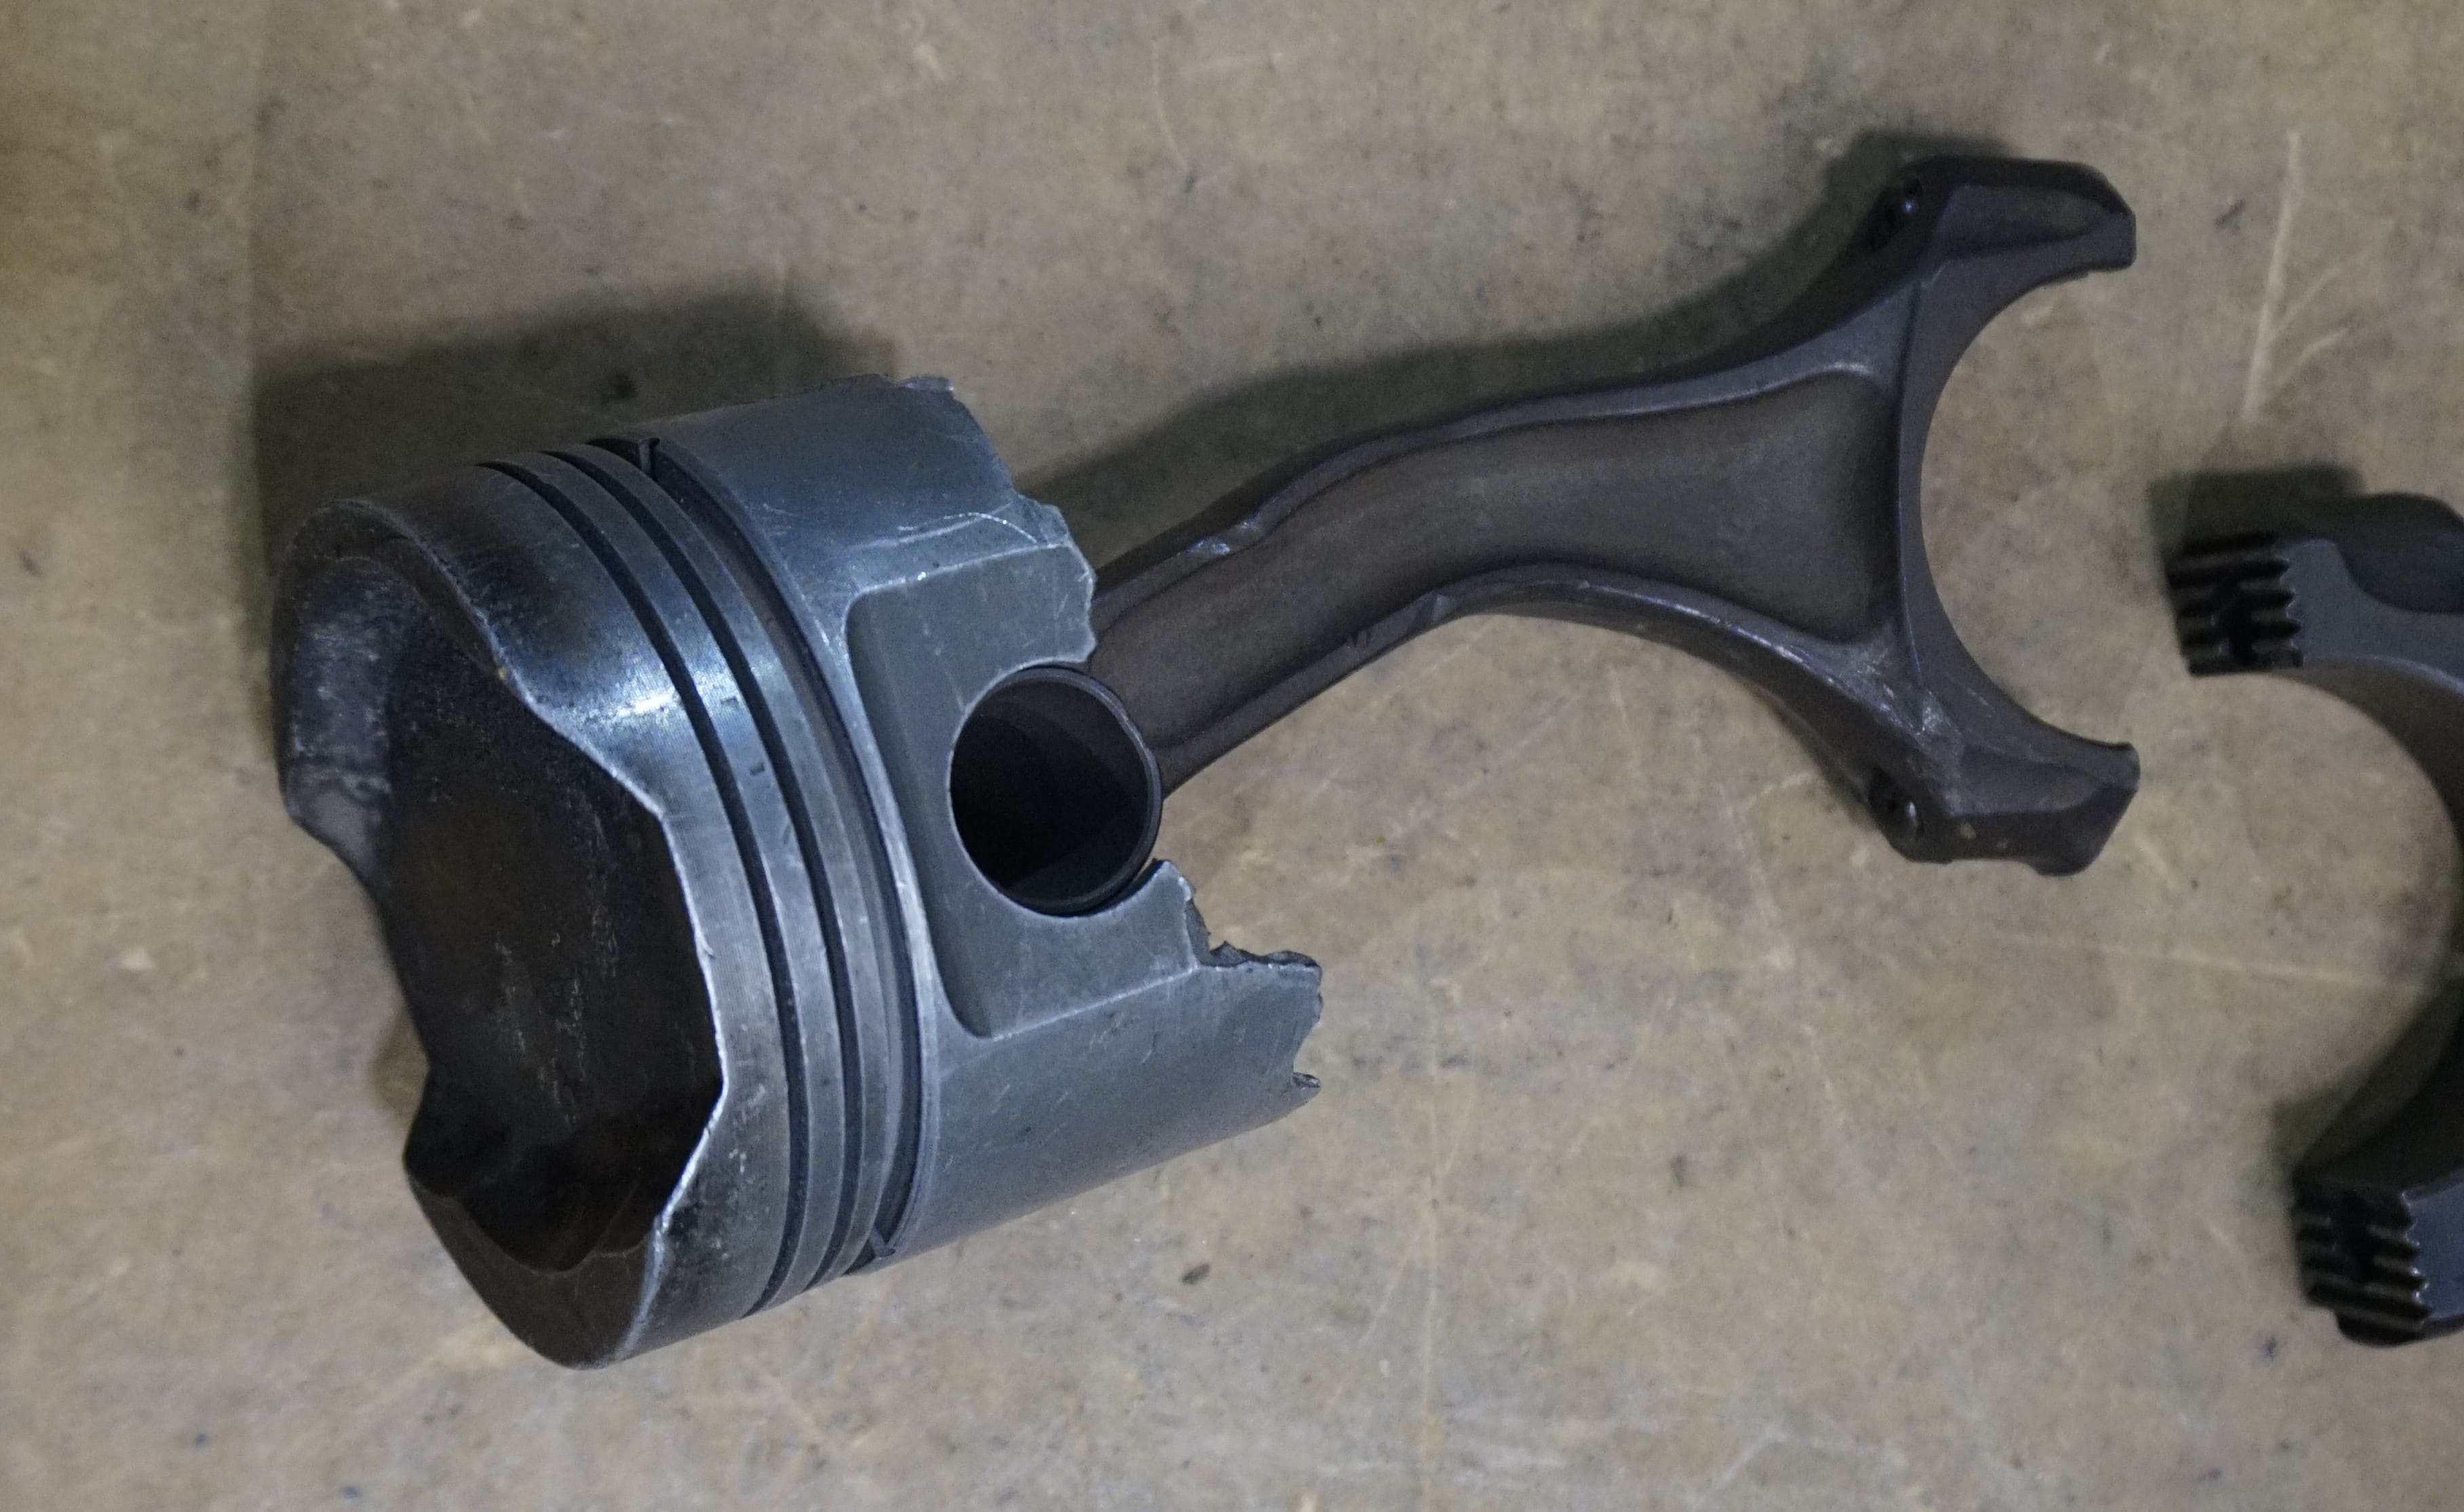
\includegraphics[width=\linewidth]{Figures/02/m4/damage.jpg}
 		\caption{Biela y pistón destruidos.}
		\label{fig:broken_w_p}
	\end{subfigure}    
	\caption{Bielas que han fallado.}
	\label{fig:broken_conrod}
\end{figure}

\subsection{Motores radiales} \label{ss:radial_conrod}

En los motores radiales, el cigüeñal y una de las bielas son una única pieza, y el resto de bielas se fijan a esa primera, permitiéndose su rotación. En la figura \ref{fig:conrod_radial} se puede ver un montaje típico de un motor de 7 cilindros radiales.

\begin{figure}[H]
	\centering
	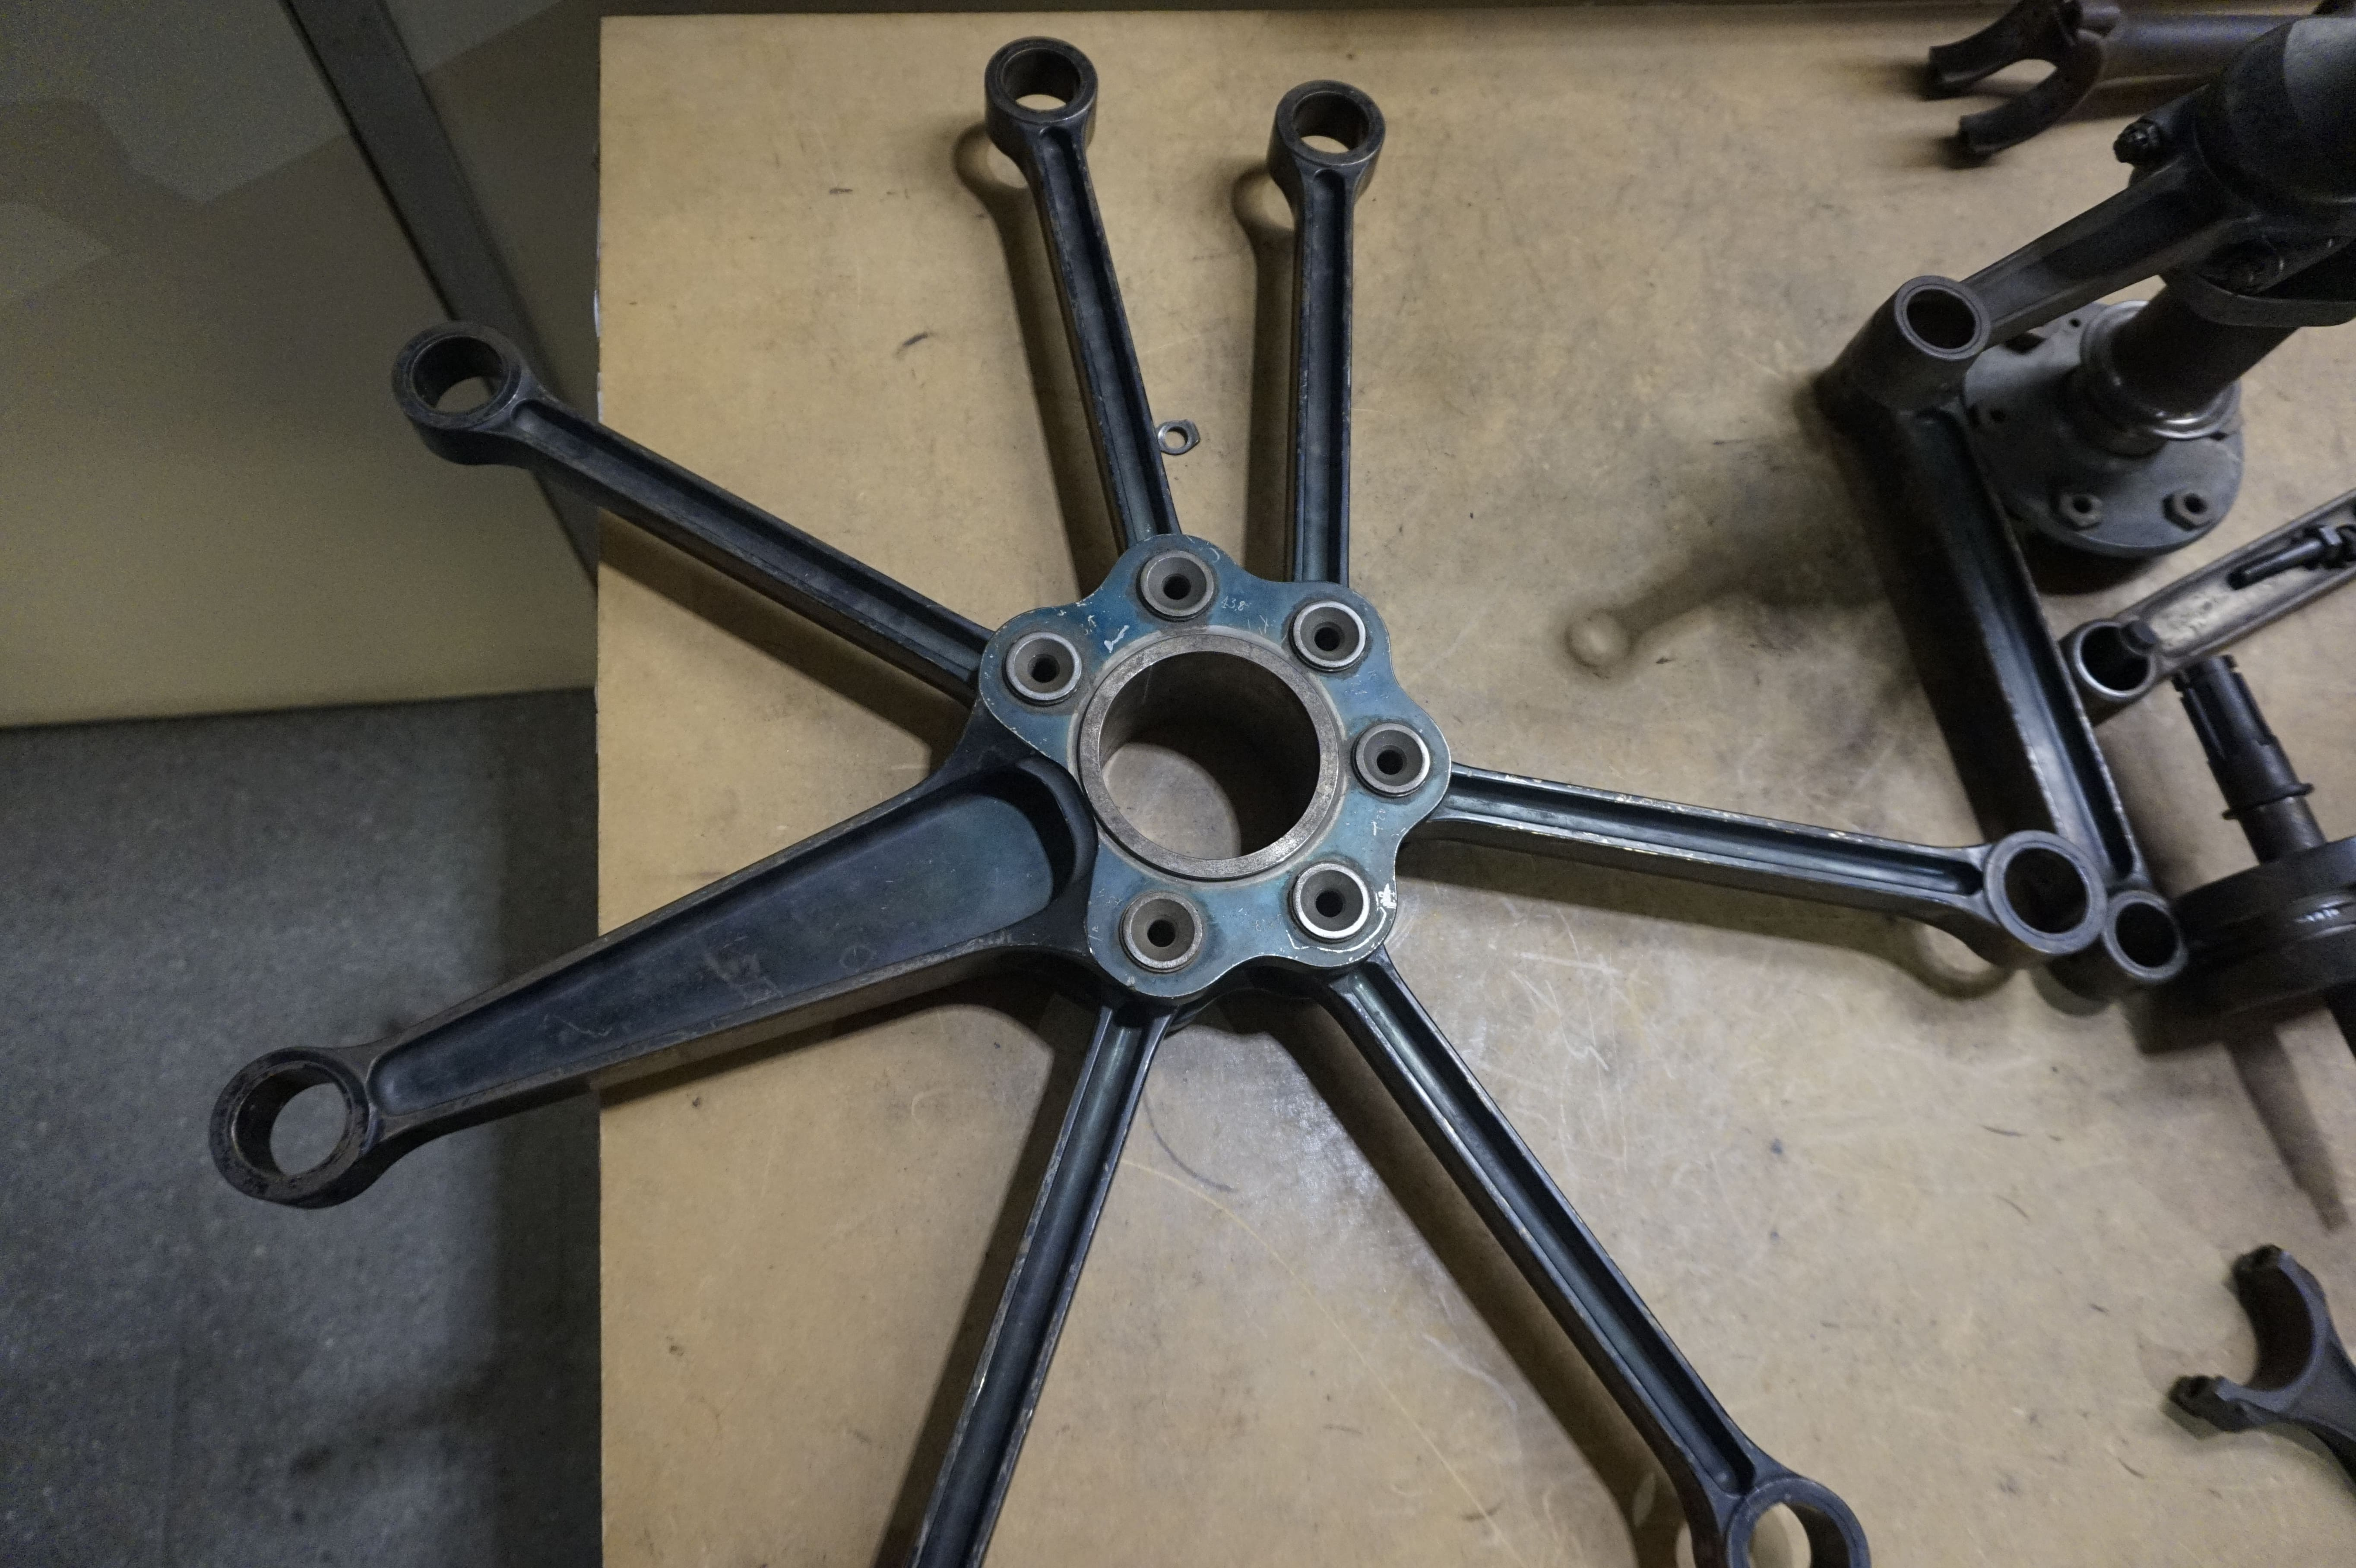
\includegraphics[width=0.6\linewidth]{Figures/02/m4/cig_radial.jpg}
	\caption{Cigüeñal de un motor radial.}
	\label{fig:conrod}
\end{figure}






%\section{Piezas adicionales} \label{s:section_05}

%En esta sección se desarrollará de manera resumida el uso de algunas piezas adicionales a las estudiadas en el resto de este presente informe.

\newpage

\section{Conclusión} \label{s:conclusion}

Mediante la realización de esta práctica, y la escritura de este informe, los alumnos hemos podido tener un contacto lo más cercano posible con piezas reales de un motor, conociendo de primera mano todos esos componentes principales que conforman un motor alternativo y que en su conjunto permiten la obtención de potencia. De esta manera, nos ha ayudado a comprender mejor el funcionamiento de cada componente del motor de una forma más práctica y visual, saliéndonos un poco del ámbito de las ecuaciones.


\begin{figure}[H]
	\centering
	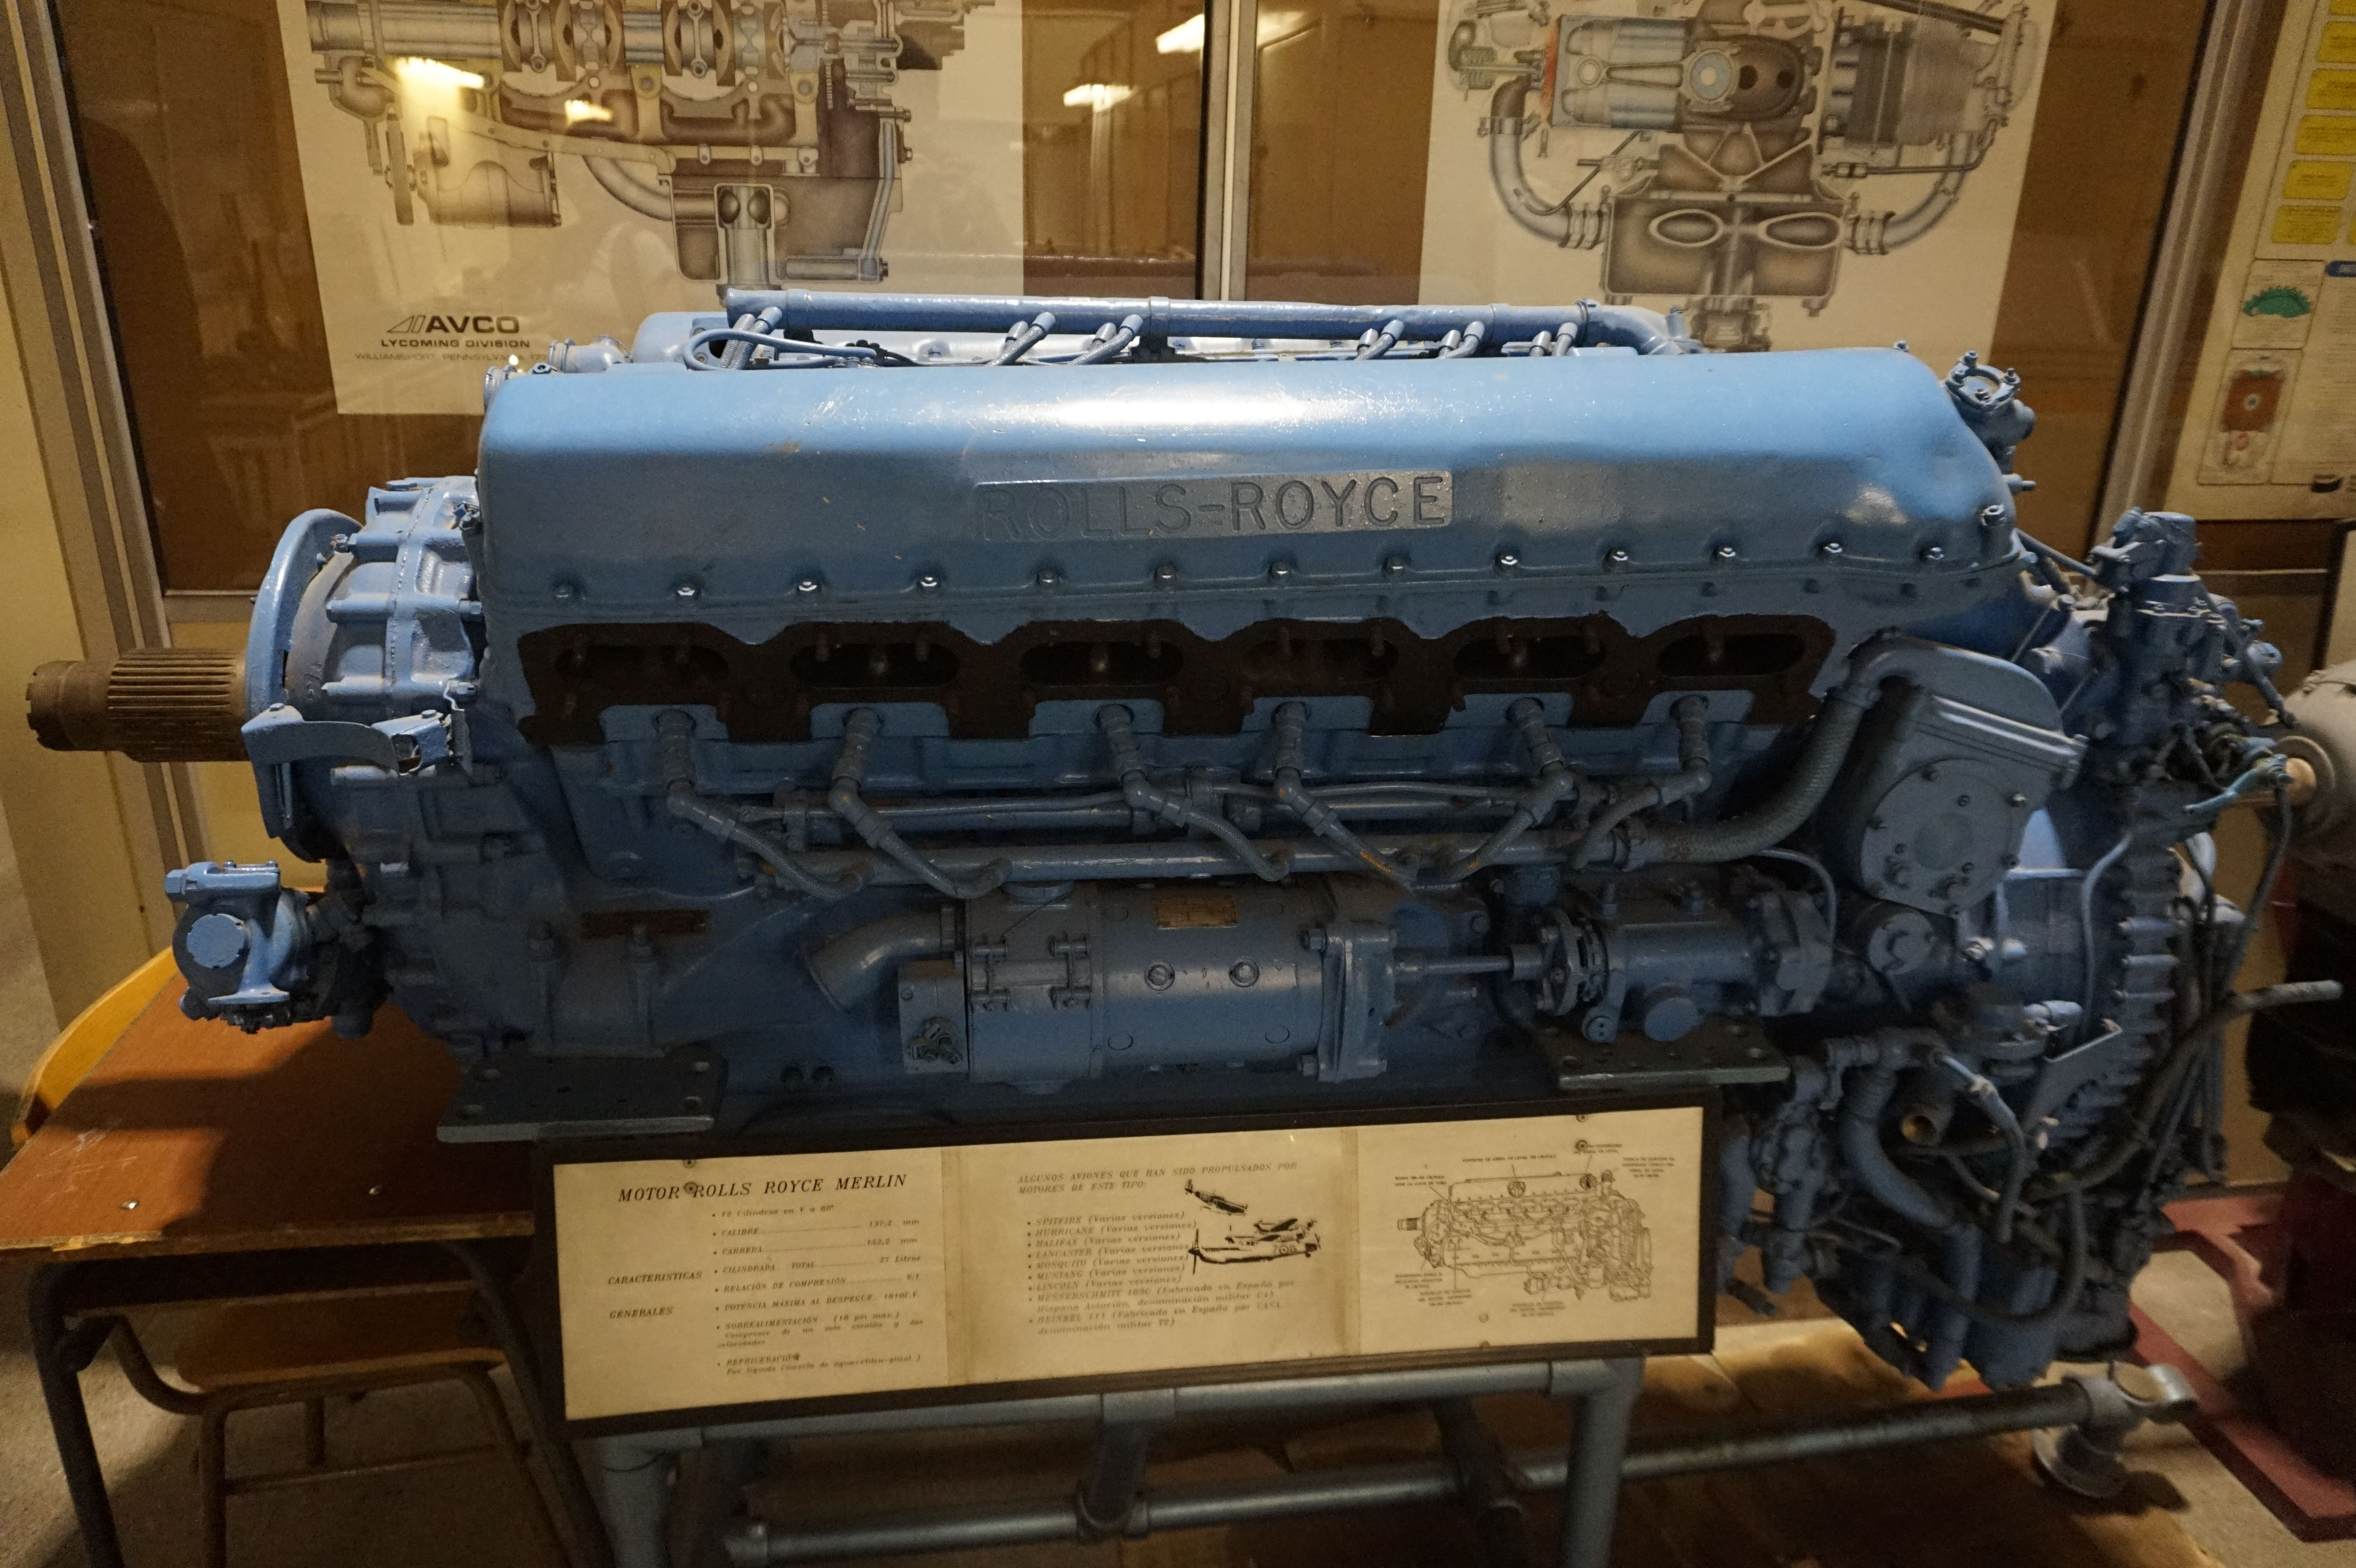
\includegraphics[width=0.6\linewidth]{Figures/02/extra/merlin.jpg}
	\caption{Motor V12 Rolls-Royce Merlin.}
	\label{fig:merlin}
\end{figure}





